\documentclass[a4paper,11pt]{memoir}

\usepackage[french]{babel}
\usepackage[utf8]{inputenc}
\usepackage[T1]{fontenc}
\usepackage{amsmath}
\usepackage{amssymb}
\usepackage{stmaryrd}
\usepackage{amsthm}
\usepackage{hyperref}
\usepackage{algorithmic}
\usepackage{algorithm}
\usepackage{graphicx}
\usepackage{dsfont}
\usepackage{fancyhdr}
\usepackage{tabulary}
\usepackage{pgfplots}
\usepackage{caption}

\captionsetup[table]{labelformat=empty}

\usepackage[explicit, clearempty]{titlesec}
%\titleformat{\chapter}[display]{\bfseries\filright}{\huge\chaptername~\thechapter}{20pt}{\Huge#1}
%\titleformat{name=\chapter, numberless}[display]{\bfseries\filright}{}{0pt}{\Huge#1}[\addcontentsline{toc}{chapter}{#1}]

\setcounter{secnumdepth}{3}
\setcounter{tocdepth}{3}

\usepackage{tocbibind}



\title{Algorithmes de simulation de champs gaussiens}
\author{Valentin Abongo}


\pagestyle{fancy}
\fancyhead{}
\fancyhead[RO,LE]{\textit{\hfill\leftmark}}
\fancyfoot[R]{\footnotesize{© Airbus SAS tous droits réservés}}

\raggedbottom

\newcommand{\ud}{\,\mathrm{d}}
\theoremstyle{definition} \newtheorem{definition}{Définition}[section]
\theoremstyle{definition} \newtheorem{theorem}{Théorème}[section]
\theoremstyle{definition} \newtheorem{corollary}{Corollaire}[section]
\theoremstyle{definition} \newtheorem{property}{Propriété}[section]
\theoremstyle{definition} \newtheorem{hypothesis}{Hypothèse}[section]
\theoremstyle{remark} \newtheorem{remark}{Remarque}[section]
%\theoremstyle{definition} \newtheorem{proof}{Preuve}[section]

\newcommand{\BEGIN}{\STATE \fbox{Début}}
\renewcommand{\algorithmicensure}{\textbf{Sortie(s)}}
\newcommand{\END}{\STATE \fbox{Fin}}
\renewcommand{\algorithmicrequire}{\textbf{Entrée(s)}}
\renewcommand{\algorithmicend}{\textbf{fin}}
\renewcommand{\algorithmicfor}{\textbf{pour}}
\renewcommand{\algorithmicto}{\textbf{à}}
\renewcommand{\algorithmicendfor}{\textbf{fin du pour}}
\renewcommand{\algorithmicdo}{\textbf{faire}}

\floatname{algorithm}{Algorithme}



\begin{document}
\maketitle
\nocite{*}
%abstract du mémoire
\begin{abstract}
On s'intéresse ici à la simulation de champs gaussiens. Il existe de multiples façons de
les simuler et l'objectif sera de faire un inventaire sur plusieurs méthodes. Les simulations qui y sont décrites
ont été testées en code python à l'aide d'une bibliothèque C++/Python du nom d'OpenTURNS\footnote{http://openturns.github.io/} dont Airbus est l'un des
contributeurs. OpenTURNS permet notamment le traitement des incertitudes à l'aide de diverses notions de statistique
et de modéliser des phénomènes aléatoires, dont les champs gaussiens. Par conséquent certaines méthodes de simulation y sont
déjà implémentées et ne nécessitent donc que de les trouver dans la bibliothèque. Cependant d'autres méthodes n'existaient pas
en soi sur OpenTURNS et elles ont mené à produire du nouveau code basé  essentiellement sur la bibliothèque.  
\end{abstract}

%\newpage


\newpage

\tableofcontents

%chapitre introductif 
\chapter{Introduction}
\label{introProb}
\section*{Problème général}


\noindent Soit $(\Omega,\mathcal{F},\mathbb{P})$ un espace probabilisé \\
Soit $n,d$ deux entiers naturels non nuls et $D$ un fermé borné de $\mathbb{R}^n$ \\
Soit $X=(X_t)_{t\in \mathbb{R}^n}$ un processus gaussien centré d'ordre 2 à valeurs dans $\mathbb{R}^d$ \\
Notons $C: \mathbb{R}^n \times \mathbb{R}^n \rightarrow M_d(\mathbb{R}) $ la fonction de covariance de $X$ \\

On souhaite simuler une réalisation du processus $X$ sur le domaine $D$. Pour~cela,
on discrétise le domaine $D$ par un maillage $M$ (de préférence une triangulation de $D$) et on
simule $X$ sur les n\oe uds du maillage $(n_i)_{i \in \llbracket 1; m \rrbracket} $ où $m$ est le nombre de noeuds. Il s'agit donc de simuler
le vecteur aléatoire $X_M=(X_{n_1},...,X_{n_m})$, qui n'est rien d'autre qu'un vecteur gaussien centré à valeurs dans $(\mathbb{R}^d)^m$
qu'on assimile à $\mathbb{R}^{dm}$. 
D'où $X_M$ est caractérisé par sa matrice de covariance $\Sigma \in M_{dm}(\mathbb{R})$ dont les coefficients sont donnés
par la fonction de covariance $C$. Plus concrètement pour $(i,k) \in \llbracket 1; m \rrbracket^2, (j,l) \in \llbracket 1; d \rrbracket^2,\; \Sigma_{(i-1)m + j, (k-1)m + l} = C(n_i,n_k)_{j,l} = \mathbb{E}((X_{n_i})_{j}(X_{n_k})_{l}) $. On a en parti\-culier que $\Sigma$ est symétrique semi-définie positive.\\

La problématique revient donc à simuler la loi $\mathcal{N}(0_{\mathbb{R}^{dm}},\Sigma)$. On présentera d'abord des méthodes classiques pour ensuite en exhiber d'autres dont l'approche 
considère davantage le type de processus que l'on cherche à simuler.
~\\

On supposera par la suite que $\Sigma$ est symétrique réelle définie positive, quitte à la régulariser\footnote{En notant $\lambda_{max}$ le module maximum du spectre de $\Sigma$,
la régularisation se fait en ajoutant une fraction $\epsilon$ de $\lambda_{max}$ sur sa diagonale i.e on ajoute $\epsilon \cdot \lambda_{max}$ aux
coefficients diagonaux de $\Sigma$}.


%les définitions de bases (peut être à mettre dans appendix)
%estimations empiriques pour valider ou non une méthode de simulation (appendix) (évoquer Box-Muller en appendix peut-être)




%chapitre Cholesky
\chapter{Simulation par méthode de Cholesky}
\label{chapCholesky}
\section{Méthode de Cholesky}

\label{choleskySection1} En utilisant les notations du chapitre~\ref{introProb}, évoquons deux propriétés qui conduisent au premier algorithme de simulation
de la gaussienne $\mathcal{N}(0_{\mathbb{R}^{dm}},\Sigma)$.


\begin{property}
  Soit $r \in \mathbb{N}^{*}$ et $U_1, \cdots, U_r$ $r$ variables aléatoires réelles iid
suivant la loi gaussienne centrée réduite $\mathcal{N}(0,1)$. Alors:
\begin{center}
$U = (U_1, \cdots, U_r) \sim \mathcal{N}(0_{\mathbb{R}^r}, I_r)$
\end{center}
\end{property}

\begin{property}
Soit  $r \in \mathbb{N}^{*}$, $V: \Omega \rightarrow \mathbb{R}^r $ un vecteur aléatoire tel que $V \sim \mathcal{N}(0_{\mathbb{R}^r},~I_r)$, $A$ une matrice de $M_{r}(\mathbb{R})$, et $L$ une matrice triangulaire inférieure de $M_{r}(\mathbb{R})$ tel que 
\begin{equation}
A = LL^{T} \label{cholesky}
\end{equation}
 
\begin{center} Alors: $LV \sim \mathcal{N}(0_{\mathbb{R}^r},A)$ \end{center}
\end{property}

\begin{remark}
  La relation~\eqref{cholesky}  est la décomposition de Cholesky de $A$ par~$L$
\end{remark}


\noindent De ces propriétés, on obtient que si $\Sigma$ admet une décomposition de Cholesky et que l'on sait simuler des réalisations indépendantes
de la loi gaussienne univariée centrée réduite, alors on peut simuler $\mathcal{N}(0_{\mathbb{R}^{dm}},\Sigma)$.\\
~\\
Par une méthode du style Box-Muller, on sait simuler des réalisations indépendantes de la loi gaussienne univariée centrée réduite.
Puis comme $\Sigma$ est symétrique définie~positive, $\Sigma$ admet une décomposition de Cholesky $LL^{T}$.
Pour obtenir cette décomposition, on utilise la méthode de Cholesky qu'on peut appliquer à toute matrice réelle symétrique définie-positive.
(voir \textbf{Algorithme \ref{algo1}}). La décomposition de Cholesky est unique du moment que l'on impose à ce que les
coefficients diagonaux de $L$ soient des réels positives, ce que garantit la méthode de Cholesky. 

Finalement si on note $\Sigma = LL^{T}$, la décomposition de Cholesky de $\Sigma$, on déduit un algorithme de simulation
de $N$ réalisations indépendantes de $X_M$ (voir \textbf{Algorithme \ref{algo2}}).
~\\

\begin{algorithm}
\caption{\textsc{Méthode de Cholesky}}
\label{algo1}
\begin{algorithmic}
\REQUIRE {$A$ une matrice symétrique définie positive de taille $r$}
\BEGIN 
\STATE {Soit $L$ une matrice nulle de taille $r$}
\FOR {j:=1 \TO $r$}
\STATE {$L[j,j] = \sqrt{A[j,j]-\displaystyle\sum_{k=1}^{j-1} |L[j,k]|^{2}}$}
\FOR {i:=j+1 \TO $r$}
\STATE {$L[i,j] = \frac{A[i,j] - \displaystyle\sum_{k=1}^{j-1} L[j,k]L[i,k]}{L[j,j]}$}
\ENDFOR
\ENDFOR
\END
\ENSURE $L$ \\
\end{algorithmic}
\end{algorithm}

~\\
~\\



\begin{algorithm}
\caption{\textsc{Algorithme de simulation}}
\label{algo2}
\begin{algorithmic}
\REQUIRE $x$ liste de longueur $N$ (nombre de réalisations), $L \in M_{dm}(\mathbb{R})$ 
\BEGIN 
\FOR {i:=1 \TO $N$}  
\STATE {on produit $y = (y_1, \cdots, y_{dm})^{T} \in \mathbb{R}^{dm}$ selon  $\mathcal{N}(0_{\mathbb{R}^{dm}},I_{dm})$}
\STATE {$x[i] = Ly \in \mathbb{R}^{dm}$ (produit matriciel de $L$ et $y$)} 
\ENDFOR
\END
\ENSURE $x$ \\
\end{algorithmic}
\end{algorithm}
~\\
En observant l'algorithme~\ref{algo2}, on saisit que la complexité en temps d'une réalisation du vecteur gaussien $\mathcal{N}(0_{\mathbb{R}^{dm}},\Sigma)$ dépend de
si la matrice $L$ a été calculée ou non. Si c'est le cas, cette complexité se veut en $O((dm)^2)$ (produit matrice-vecteur). Si ce n'est pas
le cas, il faut aussi calculer la factorisation de Cholesky et la complexité en temps devient $O((dm)^3)$. La complexité
mémoire est en $O((dm)^2)$ (stockage de $\Sigma$).
\newpage
\section{Estimation de l'erreur}

\subsection{Quantification de l'erreur}
\label{quantifErreur}
Par la suite pour $r \in \mathbb{N}^{*}$, $\mathbb{R}^r$ pourra être vu comme l'ensemble des matrices colonnes à $r$ lignes.\\

Pour savoir si le vecteur aléatoire $X_M$ est bien simulé, il faut quantifier
une erreur de simulation. La loi forte des grands nombres stipule que si l'on considère $r$ un entier non nul, $(Y_N)_{N \in \mathbb{N}^{*}}$
une suite de vecteurs aléatoires dans $L^1_{\mathbb{R}^r}(\Omega,\mathbb{P})$ iid selon la loi d'un élément $Y \in L^1_{\mathbb{R}^r}(\Omega,\mathbb{P})$, alors:
\begin{center} $\frac{1}{N}\displaystyle\sum_{i = 1}^{N} Y_i  - \mathbb{E}(Y) \xrightarrow[N \to \infty]{p.s} 0$ \end{center}

\noindent Par conséquent si on considère $(Y_N)_{N \in \mathbb{N}^{*}}$ la suite de vecteurs aléatoires modélisant des réalisations indépendantes du vecteur aléatoire $X_M$, on a:
\begin{center} $\frac{1}{N}\displaystyle\sum_{i = 1}^{N} Y_iY_{i}^{T} \xrightarrow[N \to \infty]{p.s} \mathbb{E}(X_MX_{M}^{T}) = \Sigma $ \end{center}

\noindent Donc si on munit $M_{dm}(\mathbb{R})$ de la norme de Frobenius $ \|\cdot\|_F $, on obtient la reformulation suivante:
\begin{center} $\biggl \|\frac{1}{N}\displaystyle\sum_{i = 1}^{N} Y_iY_{i}^{T} - \Sigma \biggr\|_F \xrightarrow[N \to \infty]{p.s} 0 $ \end{center}

\noindent De ce résultat, on va pouvoir quantifier l'erreur de $N$ réalisations du vecteur $X_M \sim \mathcal{N}(0_{\mathbb{R}^{dm}},\Sigma) $, $y = (y_1, \cdots, y_N) \in~(\mathbb{R}^{dm})^N$, en introduisant la définition suivante.\\


\begin{definition}
Soit $N$ un entier naturel non nul et  $(z_1, \cdots, z_N) \in (\mathbb{R}^{dm})^N$ 
~\\
On définit alors l'erreur $L^2$ (relative à $X_M$) des $N$ réalisations $z=(z_1, \cdots, z_N)$ par la quantité:

\begin{equation*}
  \epsilon(\Sigma, z) = \frac{\biggl \|\frac{1}{N}\displaystyle\sum_{i = 1}^{N} z_iz_{i}^{T} - \Sigma \biggr \|_F}{\|\Sigma \|_F}
\end{equation*}
\end{definition}
~\\
\newpage
Ainsi, si on simule bien $X_M$, on a forcément par la loi forte des grands nombres, que plus le nombre de réalisations $N$ est grand, plus $\epsilon(\Sigma, y)$ doit tendre vers $0$.
L'erreur $L^2$ est donc un moyen de vérifier numériquement si notre façon de modéliser le vecteur $X_M$ est correct.\\

\subsection{Exemple sur la méthode de Cholesky}
Présentons un exemple concret où l'erreur $L^2$ a été calculée. On simule via Cholesky un processus
gaussien centré d'ordre 2 où $n = d = 1$ et ayant pour fonction de covariance $C(x,y) = e^{-|x-y|} \text{ pour } x,y \text{ dans } \mathbb{R} $.
On choisit ici $D=[-10,10]$ et comme maillage $M$, une subdivision régulière de $D$ en $1000$ intervalles ($M$~possède donc $1001$ n\oe uds).
Dans la figure~\ref{figCholeskyRea},  une réalisation de $X_M$ a été faite en les points du maillage. 

\begin{figure}[h]
\begin{center}
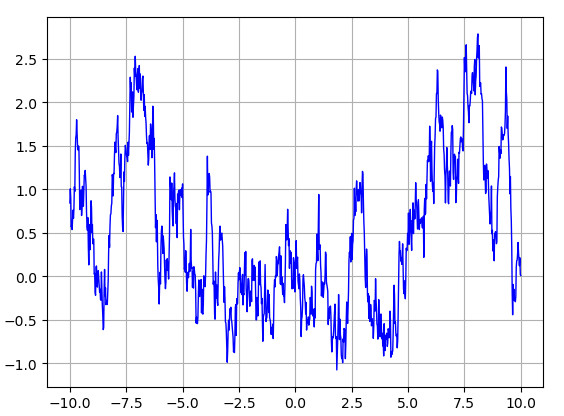
\includegraphics[scale=0.6]{images/ReaCholesky1D-1001nodes.jpg}
\caption{Réalisation du processus gaussien sur $[-10,10]$}
\label{figCholeskyRea}  
\end{center}
\end{figure}

\begin{table}[h]
\centering
\begin{tabular}{|c | c|}
\hline
Nb de réalisations & erreur $L^2$ \\
\hline
125 & 0.45627   \\
\hline
250  & 0.27285   \\
\hline
500  & 0.19814  \\
\hline
750  &  0.16260 \\
\hline
1000 &  0.15045 \\ 
\hline
\end{tabular}
\caption{Erreur $L^2$ en fonction du nombre de réalisations}
\end{table}


\begin{remark}
Le trait de la courbe de la figure~\ref{figCholeskyRea} se veut continue par interpolation linéaire en les points du maillage qui ont une valeur.
\end{remark}

\section{Erreur et convergence numérique}
\label{errConvCholesky}
La méthode de Cholesky nécessite un maillage $M$ et une fonction
de covariance $C$ pour déduire la matrice de covariance $\Sigma$. On se propose ici de décrire
les maillages et les fonctions de covariance utilisées pour les tests numériques.

\subsection{Dimension n=1}
\label{dimUnChol}
Pour les simulations, on a choisi $D = [-10,10]$. Pour $m \in \mathbb{N}^{*}, \; m > 1$,
les maillages considérés seront caractérisés à l'aide des n\oe uds du type
\begin{equation*} \biggl (t_i = -10 + \frac{20i}{m-1}\biggr)_{i \in \llbracket 0;m-1 \rrbracket}  \end{equation*}
et les éléments d'un maillage seront les intervalles de la forme $[t_i,t_{i+1}], \\i \in \llbracket 0;m-2 \rrbracket $.
On fera varier le nombre de n\oe uds $m$ entre $10$ et $10000$.\\
On n'associera à ces maillages qu'une seule fonction de covariance $C$:
\begin{equation*} C(x,y) = \exp(-|y-x|) \text{ pour } (x,y) \in \mathbb{R}^2 \end{equation*}

\begin{figure}[h]
\begin{center}
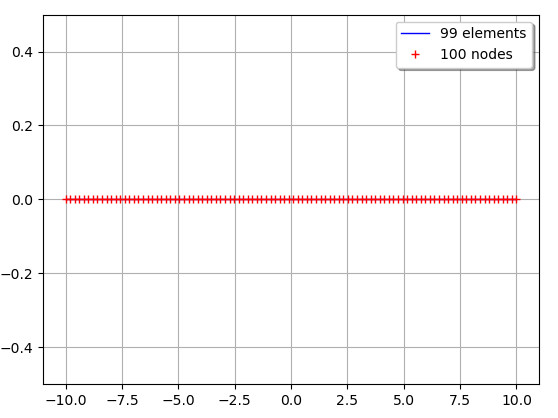
\includegraphics[scale=0.6]{images/CholeskyDim1-100.jpg}
\caption{Maillage à 100 n\oe uds en dimension 1}
\label{CholeskyMaillageDim1-100}  
\end{center}
\end{figure}


\subsection{Dimension n=2}
\label{choDim2}
En dimension 2, on a choisi $D = [-10,10]^2$. Pour $m \in \mathbb{N}^{*}, \; m > 1$,
les maillages considérés seront caractérisés par des n\oe uds du type
\begin{equation*} \biggl (t_{i,j} = (-10 + \frac{20i}{m-1}, -10 + \frac{20j}{m-1} )\biggr)_{(i,j) \in \llbracket 0;m-1 \rrbracket^2}  \end{equation*}
et par leurs éléments triangulaires dont les sommets sont décrits par des triplets
du type \begin{equation*}(t_{i,j}, t_{i+1,j}, t_{i,j+1}) \text{ ou } (t_{i+1,j}, t_{i+1,j+1}, t_{i,j+1}) , \; (i,j) \in \llbracket 0;m-2 \rrbracket^2 \end{equation*}
On fera varier le nombre de n\oe uds $m^2$ entre $10$ et $10000$.\\
On n'associera à ces maillages qu'une seule fonction de covariance $C$:
\begin{equation*} C(x,y) = \exp(-\|y-x\|_2) \text{ pour } (x,y) \in (\mathbb{R}^2)^2 \end{equation*}

\begin{figure}[h]
\begin{center}
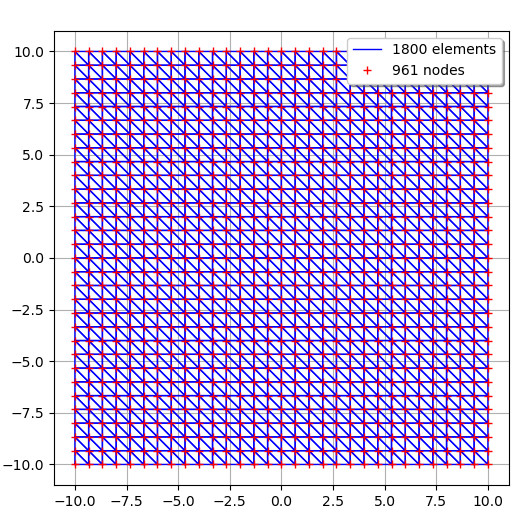
\includegraphics[scale=0.6]{images/CholeskyDim2-961.jpg}
\caption{Maillage à 961 n\oe uds en dimension 2}
\label{CholeskyMaillageDim2-961}  
\end{center}
\end{figure}

\subsection{Dimension n=3}
\label{choDim3}
En dimension 3, on a choisi $D = [-10,10]^3$. Pour $m \in \mathbb{N}^{*}, \; m > 1$,
les maillages considérés seront caractérisés par des n\oe uds du type
\begin{equation*} \biggl (t_{i,j,k} = (-10 + \frac{20i}{m-1}, -10 + \frac{20j}{m-1}, -10 + \frac{20k}{m-1} )\biggr)_{(i,j,k) \in \llbracket 0;m-1 \rrbracket^3}  \end{equation*}
et par leurs éléments tétraédriques dont les sommets sont décrits pour \\$(i,j,k) \in \llbracket 0;m-2 \rrbracket^3$ par des quadruplets ayant une de ces 6 formes:
\begin{equation*}(t_{i,j,k},\; t_{i+1,j,k},\; t_{i+1,j,k+1},\; t_{i+1,j+1,k+1}) , \end{equation*}
\begin{equation*}(t_{i,j,k},\; t_{i+1,j+1,k}, \;t_{i+1,j,k}, \;t_{i+1,j+1,k+1}) , \end{equation*}
\begin{equation*}(t_{i,j,k},\; t_{i+1,j,k+1},\; t_{i,j,k+1},\; t_{i+1,j+1,k+1}) , \end{equation*}
\begin{equation*}(t_{i,j,k},\; t_{i,j,k+1},\; t_{i,j+1,k+1}, \;t_{i+1,j+1,k+1}) , \end{equation*}
\begin{equation*}(t_{i,j,k},\; t_{i,j+1,k+1},\; t_{i,j+1,k},\; t_{i+1,j+1,k+1}) , \end{equation*}
\begin{equation*}(t_{i,j,k},\; t_{i,j+1,k},\; t_{i+1,j+1,k},\; t_{i+1,j+1,k+1}) \end{equation*}
On fera varier le nombre de n\oe uds $m^3$ entre $10$ et $10000$.\\
On n'associera à ces maillages qu'une seule fonction de covariance $C$:
\begin{equation*} C(x,y) = \exp(-\|y-x\|_2) \text{ pour } (x,y) \in (\mathbb{R}^3)^2 \end{equation*}
\phantom{oyez}

\begin{figure}[h]
\begin{center}
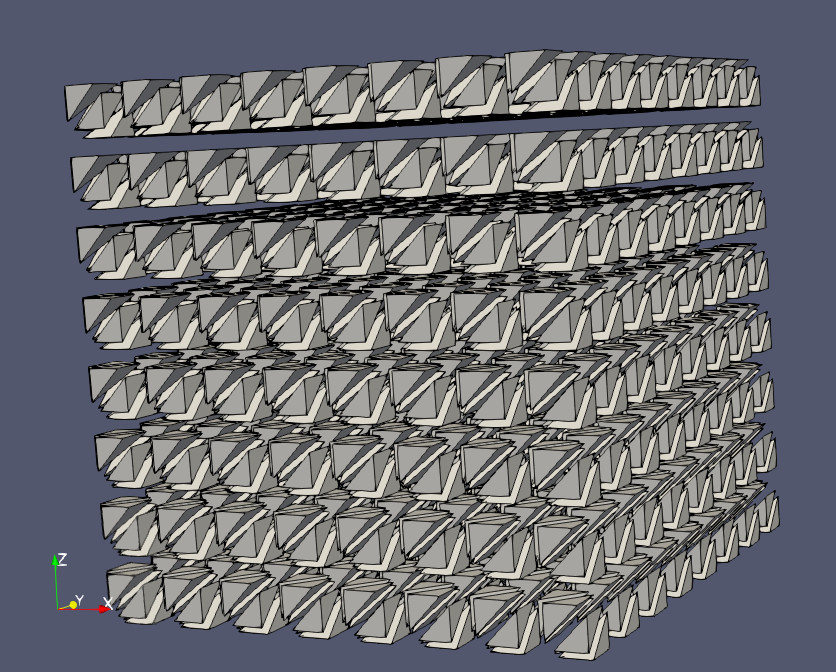
\includegraphics[scale=0.2]{images/CholeskyMaillageDim3-729.jpg}
\caption{Maillage à 729 n\oe uds en dimension 3}
\label{CholeskyMaillageDim3-729}  
\end{center}
\end{figure}


\subsection{Benchmarks}

\normalsize{
\begin{table}[htbp]
\footnotesize{
\begin{tabular}{|c |c |c |}
\hline
Dimension & Nb de n\oe uds & Temps moyen d'une réalisation (en secondes) \\
\hline
1 & 10 & 0.00020s    \\
\hline
1 & 100 & 0.00054s  \\
\hline
1 & 1000 & 0.16301s   \\
\hline
1 & 10000 & 183.51s    \\
\hline
\hline
2 & 9 & 0.00075s    \\
\hline
2 & 100 & 0.00084s    \\
\hline
2 & 961 & 0.19619s  \\
\hline
2 & 10000 & 164.28s   \\
\hline
\hline
3 & 8 & 0.00044s    \\
\hline
3 & 64 & 0.00060s    \\
\hline
3 & 729 & 0.05580s    \\
\hline
3 & 9261 & 116.86s  \\
\hline
\end{tabular}
}
%\caption{}
\end{table}
\newpage
\small{
\begin{remark}
Le nombre moyen de réalisations est estimé sur une durée de 5 secondes maximum.
Une durée supérieure à 5 secondes pointe le fait qu'une
seule réalisation a pu être effectuée et qu'elle a duré plus de 5 secondes.
Certes pour un grand maillage, la durée non négligeable de la factorisation de
Cholesky de $\Sigma$ augmente le temps de la première réalisation, mais bien souvent
les capacités limitées de la mémoire vive nécessitent de la
mémoire supplémentaire et l'accès à cette mémoire ralentit l'exécution
du code. Ceci explique notamment les temps moyens supérieures à 100 secondes. On note aussi
que pour un maillage donnée, l'erreur $L^2$ tend vers $0$ comme l'inverse de
la racine carrée du nombre de réalisations.\\
~\\
\end{remark}
}
\normalsize{}

\begin{table}[htbp]
\centering
\footnotesize{
\begin{tabular}{|c |c |c |c |c |} 
\hline
Dimension & Nb de n\oe uds & Nb de réalisations & erreur $L^2$ \\
\hline
1 & 10 & 250 & 0.14875   \\
\hline
1 & 10 & 500 & 0.12409    \\
\hline
1 & 10 & 750 &  0.09597   \\
\hline
1 & 10 & 1000 & 0.07025   \\
\hline
\hline
1 & 100 & 250 &  0.26887   \\
\hline
1 & 100 & 500 & 0.19460  \\
\hline
1 & 100 & 750 & 0.14790    \\
\hline
1 & 100 & 1000 & 0.13010    \\
\hline
\hline
1 & 1000 & 250 & 0.29682    \\
\hline
1 & 1000 & 500 & 0.18924    \\
\hline
1 & 1000 & 750 &  0.17071  \\
\hline
1 & 1000 & 1000 & 0.14616    \\
\hline
\hline
2 & 9 & 250 & 0.20574   \\
\hline
2 & 9 & 500 &  0.12867  \\
\hline
2 & 9 & 750 & 0.09212   \\
\hline
2 & 9 & 1000 & 0.09902  \\
\hline
\hline
2 & 100 & 250 & 0.45563   \\
\hline
2 & 100 & 500 & 0.31861   \\
\hline
2 & 100 & 750 & 0.26100    \\
\hline
2 & 100 & 1000 & 0.22472  \\
\hline
\hline
2 & 961 & 250 & 0.91385   \\
\hline
2 & 961 & 500 & 0.65045     \\
\hline
2 & 961 & 750 & 0.53042   \\
\hline
2 & 961 & 1000 & 0.45776    \\
\hline
\hline
3 & 8 & 250 & 0.15579  \\
\hline
3 & 8 & 500 & 0.11870    \\
\hline
3 & 8 & 750 & 0.09126    \\
\hline
3 & 8 & 1000 & 0.08644    \\
\hline
\hline
3 & 64 & 250 & 0.37056   \\
\hline
3 & 64 & 500 & 0.25594   \\
\hline
3 & 64 & 750 & 0.21249    \\
\hline
3 & 64 & 1000 & 0.18017    \\
\hline
\hline
3 & 729 & 250 & 1.1991   \\
\hline
3 & 729 & 500 & 0.84544    \\
\hline
3 & 729 & 750 & 0.69187    \\
\hline
3 & 729 & 1000 & 0.59801   \\
\hline
\end{tabular}
}
\end{table}
\normalsize{}

%\begin{remark}
%On note aussi que pour un maillage donnée, l'erreur $L^2$ tend bien vers $0$ comme l'inverse de
%la racine carrée du nombre de réalisations.
%\end{remark}


%chapitre hmatrices
\chapter{Optimisation par les $\mathcal{H}$-matrices}
\label{hmatrixchapter}
Si on reconsidère l'algorithme~\ref{algo2} de la section~\ref{choleskySection1},
et que l'on pose $r = dm$, on rappelle la nécessité de connaître la factorisation de Cholesky $L$ de la
matrice de covariance $\Sigma~\in~M_{r}(\mathbb{R}) $ pour simuler $\mathcal{N}(0_{\mathbb{R}^{r}},\Sigma)$. Contrairement aux autres
opérations qui permettent la simulation, la méthode de Cholesky qui déduit
$L$ à partir de $\Sigma$ est très coûteuse: le nombre d'opérations est en
$\mathcal{O}(r^3)$. Ce temps nécessaire
pour déterminer $L$ sera appelé le coût de démarrage.\\
On devine clairement que pour un $r$ suffisament grand (de l'ordre de $10^3$), le coût
de démarrage devient non négligeable. Par conséquent, si on veut
simuler une gaussienne, il peut vite s'avérer judicieux de
réduire ce coût. De multiples façons existent pour le faire. On se propose ici
de présenter l'une d'elles qui consiste à considérer une structure de données
qui peut permettre dans certains cas la réduction du coût de démarrage. Il
s'agit de la structure des matrices hiérarchiques ou encore $\mathcal{H}$-matrices. Elles permettent des représentations compressées de matrices denses. Cette structure ne sera pas décrite dans les détails mais tout lecteur intéressé pourra se référer à la thèse de Benoît Lizé~\cite{LizéBenoît2014Rdrp}.

\section{Idée globale des $\mathcal{H}$-matrices}

L'idée de base de la structure des $\mathcal{H}$-matrices est de pouvoir
approcher certains blocs d'une matrice par 
des matrices de la forme $AB^{T}$. Une représentation de la forme $AB^{T}$ peut réduire
le coût mémoire de la matrice. En effet si on considère $A \in M_{m,k}(\mathbb{R})$ et $B \in M_{n,k}(\mathbb{R})$ où $k \leq  \min(m,n)$, alors stocker $AB^{T}$ coûte en mémoire
$mn$ cases-mémoire alors que stocker $A$ et $B$ coûte $k(m+n)$, ce qui peut être intéressant si $k \ll \min(m,n)$.

La représentation compressée d'une matrice dense $C$ en $\mathcal{H}$-matrice nécessite deux étapes: une subdivision en plusieurs blocs de la matrice $C$ (découpage hiérarchique) puis
on compresse au format $AB^{T}$ les blocs qui sont admissibles.

Une fois que l'on obtient la représentation compressée de la matrice, il sera possible de
faire diverses opérations élémentaires d'algèbre linéaire tout en préservant la
structure de $\mathcal{H}$-matrice. Dans le cas de la simulation d'un
champ gaussien, vu que l'algorithme de simulation est le même que l'algorithme~\ref{algo2} de la section~\ref{choleskySection1}, sauf que l'on utilise la structure des $\mathcal{H}$-matrices,
deux opérations seront différentes dans leur implémentation (qu'on n'évoquera pas): la factorisation de
Cholesky et le produit matrice-vecteur.

Pour la suite, pour $M \in M_{p,q}(\mathbb{R})$, $\sigma \subset \llbracket 1;p \rrbracket$,
$\tau \subset \llbracket 1;q \rrbracket$, on note $M_{|\sigma \times \tau}$ le
bloc $\sigma \times \tau$ de la matrice $M$, $(M_{i,j})_{(i,j) \in \sigma \times \tau}$. On dira aussi que $\sigma$ est un ensemble d'indices \og ligne\fg{} et que
$\tau$ est un ensemble d'indices \og colonne\fg{}.


\begin{figure}[h]
\begin{center}
\includegraphics[scale=0.6]{images/représentationCompressionHmatrice.jpg}
\caption{Compression au format $AB^{T}$}
\label{ideeCompressionHmatrice}  
\end{center}
\end{figure}

\section{Compression en $\mathcal{H}$-matrice}

\subsection{Découpage hiérarchique}

Dans cette sous-section, on emploiera du vocabulaire propre à la théorie
des graphes, notamment le concept d'arbre. \` A la page 66 de la thèse de Lizé,
il est possible de se familiariser avec ce vocabulaire.\\

Considérons $m,d$ et $N_{leaf}$ 3 entiers non nuls, $M \in M_{m}(\mathbb{R})$ une matrice carré. On suppose de plus qu'à chaque indice $j$ de l'ensemble
$\llbracket 1;m \rrbracket$, on associe un vecteur $x^j \in \mathbb{R}^d$ (dont on note sa $i$\up{ème} coordonnée $(x^j)_i$).  On peut voir les $x^j$ comme associés aux n\oe uds d'un maillage mais
on ne va pas jusqu'à supposer que les $x^i$ sont deux à deux distincts.
Notons par ailleurs $\mathcal{I}=\llbracket 1;m \rrbracket$.


\begin{remark}
\label{assignIndexLogic}
Si on réutilise les notations du chapitre~\ref{introProb} pour le temps de cette remarque et
que l'on reconsidère la matrice de covariance $\Sigma \in M_{dm}(\mathbb{R})$,
en raison de sa définition, pour chaque indice $i$ de l'ensemble
$\llbracket 1;dm \rrbracket$, on peut associer de façon logique un n\oe ud du maillage $M$.
En effet pour $i \in \llbracket 1; m \rrbracket, j \in \llbracket 1; d \rrbracket$,
on associe à l'indice $(i-1)m + j \in \llbracket 1;dm \rrbracket$, le n\oe ud $n_i$.
\end{remark}
\subsubsection{Découpage hiérarchique de l'espace}
\label{DecoupHieSpace}
\noindent Pour cette première étape, l'idée est de construire récursivement à partir de
la racine, un arbre $\mathcal{T}_{\mathcal{I}}$ dont les sommets sont des parties de $\llbracket 1;m \rrbracket$ (donc des ensembles d'indices).  L'arbre obtenu est un Cluster Tree (ou
arbre de groupes). La racine de l'arbre sera l'ensemble $\llbracket 1;m \rrbracket$. Afin de construire l'arbre, on a besoin d'une fonction
\og $\mathrm{Split}$ \fg{} qui à partir d'un ensemble d'indices $\sigma$, produit une partition de $\sigma$,
$\sigma_1, \cdots, \sigma_l$, où $l$ est en général fixé. Quand $l$ vaut $2$ on obtient un arbre binaire. Par ailleurs, on contraint à ce que toutes
les feuilles de $\mathcal{T}_{\mathcal{I}}$ soient des ensembles d'indices de cardinal
inférieur ou égal à $N_{leaf}$. \\ La construction du Cluster Tree est donnée par l'algorithme~\ref{algoClustTree} où pour
un sommet $\sigma$ de l'arbre, on notera $\mathrm{S}(\sigma)$ l'ensemble des fils
du sommet $\sigma$. Donc en particulier, si $\sigma$ est une feuille, $\mathrm{S}(\sigma)$ est l'ensemble vide.
\begin{remark}
Les feuilles de $\mathcal{T}_{\mathcal{I}}$ forment une partition de $\mathcal{I}$.   
\end{remark}


\begin{algorithm}
\caption{\textsc{Création du Cluster Tree}}
\label{algoClustTree}
\begin{algorithmic}
\STATE {\textbf{déf} createClusterTree($\sigma$) }
\STATE {\quad \textbf{si} $|\sigma| \leq N_{leaf}$ \textbf{alors} }
\STATE {\quad \quad $\mathrm{S}(\sigma) = \varnothing$ }
\STATE {\quad \textbf{sinon}}
\STATE {\quad \quad $\sigma_1, \cdots, \sigma_l = \mathrm{Split}(\sigma)$ }
\STATE {\quad \quad $\mathrm{S}(\sigma) = \{\sigma_1, \cdots, \sigma_l \}$}
\STATE {\quad \quad createClusterTree($\sigma_1$)}
\STATE {\quad \quad $\cdots$}
\STATE {\quad \quad createClusterTree($\sigma_l$)}
\END
\end{algorithmic}
\end{algorithm}

Pour la fonction \og $\mathrm{Split}$ \fg{} qui forme une partition, on évoquera deux choix possibles de fonction: le découpage
médian et le découpage géométrique. Si on considère $\sigma \subset \llbracket 1;m \rrbracket$, le début
des deux découpages est similaire: posons pour $i \in \llbracket 1;d \rrbracket$,
$x_{min,\sigma}^{i} = \min_{j \in \sigma} (x^j)_i $ et $x_{max,\sigma}^{i} = \max_{j \in \sigma} (x^j)_i $.
La première étape consiste à déterminer $i^{*} \in \llbracket 1;d \rrbracket$ tel que
$x_{max,\sigma}^{i^{*}} - x_{min,\sigma}^{i^{*}}$ soit de valeur maximale (on détermine donc l'axe où la boîte englobante
associée au $(x^j)_{j \in \sigma}$ est de largeur maximale).\\
La seconde étape produit la partition de
$\sigma$. Pour le découpage médian, on obtient la partition de $\sigma$, $\sigma_1$ et $\sigma_2$,
telle que si on note $x_{med,\sigma}^{i^{*}}$ la médiane de l'ensemble $\{(x^j)_{i^{*}}, j \in \sigma \}$, alors
pour $k \in \sigma$, $k$ est dans $\sigma_1$ si $(x^k)_{i^{*}} \leq x_{med,\sigma}^{i^{*}}$, sinon $k$ est dans $\sigma_2$.
Pour le découpage géométrique, on obtient la partition de $\sigma$, $\sigma_1$ et $\sigma_2$,
telle que si on note $x_{geo,\sigma}^{i^{*}} = (x_{min,\sigma}^{i^{*}} + x_{max,\sigma}^{i^{*}})/2$ alors
pour $k \in \sigma$, $k$ est dans $\sigma_1$ si $(x^k)_{i^{*}} \leq x_{geo,\sigma}^{i^{*}}$, sinon $k$ est dans $\sigma_2$.

\subsubsection{Découpage hiérarchique de la matrice}
\label{decoupHieMat}
Le découpage hiérarchique de la matrice consiste à construire à partir de $\mathcal{T}_{\mathcal{I}}$, un arbre
$\mathcal{T}_{\mathcal{I} \times \mathcal{I}}$ dont les sommets sont des parties de $\mathcal{I} \times \mathcal{I}$ de la forme $\sigma \times \tau$.
Ainsi, chaque sommet $\sigma \times \tau$ de l'arbre $\mathcal{T}_{\mathcal{I} \times \mathcal{I}}$ peut être associé au bloc $M_{|\sigma \times \tau}$
de la matrice $M$. Un tel arbre sera qualifié de Block Cluster Tree et la racine sera l'ensemble $\mathcal{I} \times \mathcal{I}$.
Pour décrire la construction de $\mathcal{T}_{\mathcal{I} \times \mathcal{I}}$,
il sera nécessaire d'introduire une fonction booléenne $f: \mathcal{P}(\mathcal{I}) \times \mathcal{P}(\mathcal{I}) \rightarrow \{0,1\}$
qui sera notre critère d'admissibilité. Plus exactement, on dira qu'un bloc $\sigma \times \tau$ est admissible si $f(\sigma,\tau) = 1$.
La construction de $\mathcal{T}_{\mathcal{I} \times \mathcal{I}}$ est décrite par l'algorithme~\ref{algoBlockClustTree} où la notation $\mathrm{S}(\sigma \times \tau)$
désignera les fils du sommet $\sigma \times \tau$ dans l'arbre $\mathcal{T}_{\mathcal{I} \times \mathcal{I}}$ tandis que la notation $\mathrm{S}(\sigma)$
désignera les fils du sommet $\sigma$ dans l'arbre $\mathcal{T}_{\mathcal{I}}$.

\begin{algorithm}
\caption{\textsc{Création du Block Cluster Tree}}
\label{algoBlockClustTree}
\begin{algorithmic}
\STATE {\textbf{déf} createClusterTree($\sigma \in \mathcal{T}_{\mathcal{I}}$, $\tau \in \mathcal{T}_{\mathcal{I}}$)}
\STATE {\quad \textbf{si} $f(\sigma,\tau) ==1$ ou $\mathrm{S}(\sigma) == \varnothing$ ou $\mathrm{S}(\tau) == \varnothing$  \textbf{alors} }
\STATE {\quad \quad $\mathrm{S}(\sigma \times \tau) = \varnothing$ }
\STATE {\quad \textbf{sinon}}
\STATE {\quad \quad $\mathrm{S}(\sigma \times \tau) = \{ \sigma^{\prime} \times \tau^{\prime},\; \sigma^{\prime} \in \mathrm{S}(\sigma) \text{ et } \tau^{\prime} \in \mathrm{S}(\tau) \}$ }
\STATE {\quad \quad \textbf{pour} $\sigma^{\prime} \times \tau^{\prime} \in \mathrm{S}(\sigma \times \tau)$ }
\STATE {\quad \quad \quad createClusterTree($\sigma^{\prime}$,$\tau^{\prime}$)}
\END
\end{algorithmic}
\end{algorithm}
  

Une fois que l'on obtient $\mathcal{T}_{\mathcal{I} \times \mathcal{I}}$, on remarque que si un sommet $\sigma \times \tau$ est admissible alors c'est une feuille.
On espère de façon générale que les feuilles admissibles soient des blocs de grande taille et que $N_{leaf}$ ait été choisi suffisamment petit
pour que les feuilles non admissibles soient de petites taille.
Finalement grâce à $\mathcal{T}_{\mathcal{I} \times \mathcal{I}}$, pour $\sigma \times \tau$ une feuille admissible, le bloc $M_{|\sigma \times \tau}$ de la matrice $M$
subira une compression pour être au format $AB^{T}$.\\

Pour la fonction booléenne $f$, son choix dépend du type de matrice que l'on considère et aussi du type de compression des blocs admissibles. On se contentera
donc d'exposer rapidement un critère d'admissibilité évoqué dans la thèse de Lizé. On définit pour $\sigma, \tau \subset \mathcal{I}$,
\begin{equation}
 \mathrm{diam}(\sigma)= \sqrt{\displaystyle\sum_{i=1}^{d} (x_{max,\sigma}^{i} - x_{min,\sigma}^{i})^2}
\end{equation}

\begin{equation}
 \mathrm{d}(\sigma,\tau) = \sqrt{\displaystyle\sum_{i=1}^{d} \max(0,x_{min,\tau}^{i} - x_{max,\sigma}^{i})^2 + \max(0,x_{min,\sigma}^{i} - x_{max,\tau}^{i})^2 } 
\end{equation}

\noindent $\mathrm{diam}(\sigma)$ désigne le diamètre de la boîte englobant les points $(x^j)_{j \in \sigma}$ et $\mathrm{d}(\sigma,\tau)$ désigne la
distance des faces les plus proches des deux boîtes englobantes associées à $\sigma$ et à $\tau$. Sous ces définitions,
il est maintenant possible de définir pour $\eta \in \mathbb{R}^{*}_{+}$ un critère d'admissibilité $f_{\eta}$: pour
$\sigma, \tau \subset \mathcal{I}$:
\begin{equation}
  \label{critAdmi}
  f_{\eta}(\sigma,\tau) =
  \begin{cases}
    1 & \quad \text{si } \min(\mathrm{diam}(\sigma),\mathrm{diam}(\tau)) < \eta \cdot \mathrm{d}(\sigma,\tau)\\
    0 & \quad \text{sinon}  \end{cases}
\end{equation}

\noindent $\eta$ est parfois appelé facteur d'admissibilité.\\


\begin{remark}
  Les feuilles de $\mathcal{T}_{\mathcal{I} \times \mathcal{I}}$ forment une partition de  $\mathcal{I} \times \mathcal{I}$. La représentation
  en $\mathcal{H}$-matrice consiste alors à stocker la matrice $M$ au niveau des feuilles de l'arbre $\mathcal{T}_{\mathcal{I} \times \mathcal{I}}$ où
  une feuille $\sigma \times \tau$ stockera aussi le sous-bloc $M_{|\sigma \times \tau}$ de la matrice $M$. Si de plus la feuille est admissible,
  alors on stockera $A$ et $B$ deux matrices issues de la compression et vérifiant $M_{|\sigma \times \tau} \approx AB^{T}$.
\end{remark}


\subsection{Compression des blocs admissibles}
\label{compBlocAdmi}
Si on considère $\sigma \times \tau$ un bloc admissible, alors on
espère que l'on dispose de $k \in \mathbb{N}^{*}$ vraiment plus petit que
$|\sigma|$ et $|\tau|$, de $A \in M_{|\sigma|,k}(\mathbb{R})$ et $B \in M_{|\tau|,k}(\mathbb{R})$ tels que $M_{|\sigma \times \tau} \approx AB^{T}$ au sens d'une norme
matricielle (on ne considérera que la norme spectrale $\|\cdot\|_2$ et la
norme de Frobenius $\|\cdot\|_F$). La représentation approchée de $M_{|\sigma \times \tau}$ par $AB^{T}$ est qualifiée de $\mathcal{R}k$-Matrice. Le théorème qui
suit présente la meilleure façon d'approcher une matrice par une
$\mathcal{R}k$-Matrice (SVD ou décomposition en valeurs singulières).

\begin{theorem}
  Soit $(p,q) \in (\mathbb{N}^{*})^2$, $A \in M_{p,q}(\mathbb{R})$. On
  note $A = U\Sigma V^{T}$ une décomposition en valeurs singulières de $A$ où
  $U \in M_{p,p}(\mathbb{R})$ et $V \in M_{q,q}(\mathbb{R})$ sont unitaires
  et $\Sigma \in M_{p,q}(\mathbb{R})$ est nulle sauf au niveau de sa diagonale
  et ses éléments diagonaux sont des réels positifs classés par ordre
  décroissant (ce sont les valeurs singulières).\\

  \noindent Soit $k \in \llbracket 1;\min(p,q) \rrbracket$. On note
  $\mathrm{diag}_{k}(\Sigma)$ la matrice $\Sigma$ où pour
  $i$ entier strictement plus grand que $k$,
  $\sigma_{i}=\Sigma_{i,i}$ a été remplacé par $0$.\\
  Alors si on note $\|\cdot\|$ la norme de Frobenius ou la norme spectrale,
  on a:
\begin{equation*}
\|A - U\mathrm{diag}_{k}(\Sigma)V^{T}\| = \min \{ \|A - R\|, \; R \in M_{p,q}(\mathbb{R}) \text{ tel que }\; \mathrm{rang}(R) \leq k \}
\end{equation*}
\noindent On a de plus:

\begin{equation}
  \label{approSpec}
\min \{ \|A - R\|_{2}, \; R \in M_{p,q}(\mathbb{R}) \text{ tel que }\; \mathrm{rang}(R) \leq k \} = \sigma_{k+1}^2
\end{equation}

\begin{equation}
  \label{approFrob}
\min \biggl \{ \|A - R\|_{F}^2, \; R \in M_{p,q}(\mathbb{R}) \text{ tel que }\; \mathrm{rang}(R) \leq k \biggr \} = \displaystyle\sum_{i=k+1}^{\min(p,q)} \sigma_{i}^2
\end{equation}
\end{theorem}


\begin{remark}
Les formules~(\ref{approSpec}) et~(\ref{approFrob}) montrent que
l'erreur d'approximation est complétement controlée par les valeurs singulières de $A$.
\end{remark}

\begin{remark}
On observe que $U\mathrm{diag}_{k}(\Sigma)V^{T}=PQ^{T}$ où $P=U\mathrm{diag}_{k}(\Sigma)$ et $Q=V$. D'où en plus d'être une $\mathcal{R}k$-Matrice,
$U\mathrm{diag}_{k}(\Sigma)V^{T}$ est une approximation optimale de $A$ par une matrice de rang au plus $k$.
Rajoutons que si on note $U_k \in M_{p,k}(\mathbb{R})$ (resp. $V_k \in M_{q,k}(\mathbb{R})$) la
matrice $U$ (resp. $V$) dont on ne retient que les $k$ premières colonnes. alors on a la représentation tronquée de rang $k$,
$U\mathrm{diag}_{k}(\Sigma)V^{T}= U_k\mathrm{diag}_{k}(\Sigma)V_{k}^{T} $, ce qui amène lorsque $k$ est connu à remplacer $U$ et $V$ par $U_k$ et $V_k$.\\
\end{remark}

En pratique, pour quantifier l'erreur, on utilise la norme de Frobenius et on a une quantité $\epsilon \in \mathbb{R}^{*}_{+}$ qui
est l'erreur absolue à ne pas dépasser. Ainsi si on reconsidère la matrice $A$ du théorème précédent, la méthode SVD conditionnée par $\epsilon$ consiste à déterminer
d'abord une décomposition en valeurs singulières (SVD)
de la matrice $A$ puis à choisir le rang $k$ comme étant le plus petit entier entre $1$ et $\min(p,q)$ tel que:
\begin{equation*} \|A - U\mathrm{diag}_{k}(\Sigma)V^{T}\|_{F} \quad = \quad \sqrt{\displaystyle\sum_{i=k+1}^{\min(p,q)} \sigma_{i}^2} \quad \leq \quad \epsilon \end{equation*}
Si les blocs admissibles sont compressés par la méthode SVD conditionnée par $\epsilon$, on appelle alors $\epsilon$ epsilon d'assemblage.\\
Cependant effectuer la SVD de la matrice $A$ admet une complexité en temps en $\mathcal{O}(pq^2 + p^2q)$. Donc compresser les blocs admissibles
par SVD pour obtenir pour chaque bloc une représentation tronquée conditionnée par l'erreur absolue $\epsilon$ peut s'avérer coûteux. C'est pourquoi il est préférable
d'opter pour un autre moyen de compression.\\

Les méthodes populaires de compression sont les méthodes ACA (Adaptive Cross Approximation). Ces méthodes
consistent à approcher une matrice $A \in M_{p,q}(\mathbb{R})$ par des approximations successives de rang $1$, $R_1 = C_1D_{1}^{T},  R_2 = C_2D_{2}^{T}, \cdots$
où les $C_i$ (resp. $D_i$) sont des vecteurs colonnes de taille $p$ (resp. de taille $q$)
et on cherche le plus petit entier $k$ vérifiant un certain critère d'arrêt pouvant être par exemple
\begin{equation} \|A - \displaystyle\sum_{i=1}^{k} R_i \|_{F} \leq \epsilon_1  \label{ACAcrit}\end{equation}
où $\epsilon_1 \in \mathbb{R}^{*}_{+}$ (appelé epsilon d'assemblage si on utilise ce critère pour compresser les blocs admissibles).
L'approximation de $A$, $\tilde{A}$, est définie ainsi \begin{equation*}\tilde{A} = \displaystyle\sum_{i=1}^{k} R_i \end{equation*}
$\tilde{A}$ est bien une $\mathcal{R}k$-Matrice car si on pose
\begin{equation*} C = \begin{pmatrix} C_1 & C_2 & \cdots & C_k \end{pmatrix} \text{ et } D = \begin{pmatrix}
    D_{1} & 0_{M_{q,1}(\mathbb{R})} & \cdots & 0_{M_{q,1}(\mathbb{R})} \\
    0_{M_{q,1}(\mathbb{R})} & D_{2} & \cdots & 0_{M_{q,1}(\mathbb{R})} \\
    \vdots & \vdots & \ddots & \vdots \\
    0_{M_{q,1}(\mathbb{R})} &  0_{M_{q,1}(\mathbb{R})} & \cdots & D_{k}
    \end{pmatrix}
   \end{equation*} alors \begin{equation*}\tilde{A} = CD^{T} \end{equation*}

Rajoutons qu'afin de réduire le rang de la matrice $\tilde{A}$ obtenue par une méthode ACA, il est possible d'appliquer une recompression de la matrice $\tilde{A}$
par une variante de la SVD (voir les pages de 58 à 60 de \cite{LizéBenoît2014Rdrp}). Dans cette variante, on applique un moment donné la méthode SVD conditionnée par un réel
strictement positif $\epsilon$ que l'on appelle epsilon de recompression.\\

Parmi les méthodes ACA, citons l'ACA pivotage total, l'ACA pivotage partiel, l'ACA+. Ces 3
méthodes sont évoquées dans la thèse de Lizé \cite{LizéBenoît2014Rdrp}.


\section{Complexité spatiale et temporelle}
L'algorithme~\ref{algo2} version $\mathcal{H}$-matrice pour une réalisation
nécessite plusieurs étapes: compresser en $\mathcal{H}$-matrice de la matrice de covariance $\Sigma \in M_{r}(\mathbb{R})$ où $r=dm$ (cette phase s'appelle aussi assemblage),
obtenir $L$, la factorisation de Cholesky version $\mathcal{H}$-matrice de $\Sigma$,
faire une réalisation $y$ du vecteur gaussien de loi $\mathcal{N}(0,I_{r})$,
et enfin faire le produit matrice-vecteur $Ly$.
~\\

La connaissance de la complexité en temps et en espace de ces étapes
permettrait d'obtenir celles de l'algorithme de simulation par
$\mathcal{H}$-matrice et on s'attend à ce qu'une forte compression de la matrice de
covariance réduise les coûts de temps et de mémoire. Cependant
cette compression dépend entre autres du type de matrices que l'on considère et
du découpage spatial. Par conséquent on ne peut donner de façon générale
la complexité en temps et en espace de l'algorithme~\ref{algo2} version $\mathcal{H}$-matrice pour une réalisation. Cependant en se référant à~\cite{LizéBenoît2014Rdrp},
on peut espérer pour certaines matrices une complexité spatiale de l'algorithme de simulation en $O(rlog(r))$ et une complexité temporelle en $O(r.log^2(r))$.

\begin{figure}[h]
\begin{center}
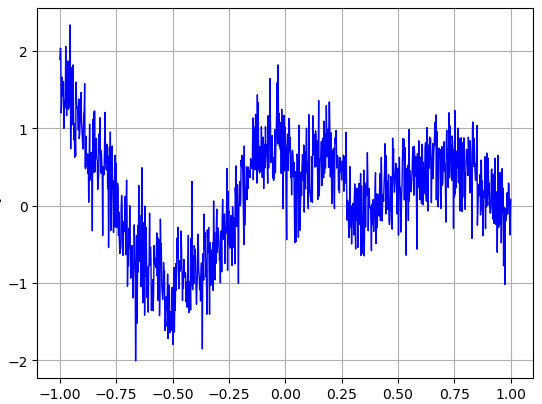
\includegraphics[scale=0.45]{images/hmatrixRea.jpg}
\caption{Réalisation sur $[-1,1]$ par méthode des $\mathcal{H}$-matrices}
\label{figHmatrixRea}  
\end{center}
\end{figure}

\newpage
\section{Erreur et convergence numérique}
\label{hmatrixerrconv}


\subsection{Paramétrage pour les tests}

Pour les tests numériques, la méthode des $\mathcal{H}$-matrices nécessite d'abord
l'information d'un maillage $M$ et d'une fonction de covariance $C$. Afin de comparer
cette méthode avec celle de Cholesky, on choisit que le choix des maillages pour
les dimensions 1, 2 et 3 et celui des fonctions de covariance seront les mêmes que ceux décrits
pour la méthode de Cholesky à la section~\ref{errConvCholesky} du chapitre~\ref{chapCholesky}. Cependant dans les sections précédentes on a vu que d'autres paramètres entraient en jeu,
en raison de la compression en $\mathcal{H}$-matrice de la
matrice de covariance $\Sigma \in M_{dm}(\mathbb{R})$. Pour que la compression soit possible, on
associe à chaque indice $i \in \llbracket 1;dm \rrbracket$ un n\oe ud du maillage $M$ en suivant la logique évoquée à la remarque~\ref{assignIndexLogic}. \\

Ces nouveaux paramètres ont été fixés de
façon identique pour tous les maillages et fonctions de covariance sélectionnés pour les tests: le paramètre $N_{leaf}$ (voir la sous-sous-section~\ref{DecoupHieSpace}) est fixé à $250$ et le type de découpage hiérarchique de l'espace sera le découpage médian. Pour le découpage
hiérarchique de la matrice (voir la sous-sous-section~\ref{decoupHieMat}), le critère
d'admissibilité (fonction booléenne) est la fonction définie par la formule~\eqref{critAdmi}
dont le facteur d'admissibilité $\eta$ est fixé à 100. Pour la compression des blocs
admissibles (voir la sous-section~\ref{compBlocAdmi}), on choisit la méthode ACA+
dont l'epsilon de recompression $\epsilon_1$ est fixé à $10^{-7}$ (voir formule~\eqref{ACAcrit}). Les blocs admissibles subiront après la méthode ACA+, une autre recompression par la
variante de la SVD où l'epsilon de recompression est fixé à $10^{-7}$.

\subsection{Benchmarks}

\begin{table}[htbp]
\centering
\begin{tabular}{|c |c |c |}
\hline
Dimension & Nb de n\oe uds & Temps moyen d'une réalisation (en seconde) \\
\hline
1 & 10 & 0.00014s    \\
\hline
1 & 100 & 0.00076s  \\
\hline
1 & 1000 & 0.07200s   \\
\hline
1 & 10000 & 0.55147s    \\
\hline
\hline
2 & 9 & 0.00024s    \\
\hline
2 & 100 & 0.00095s    \\
\hline
2 & 961 & 0.08200s  \\
\hline
2 & 10000 & 6.2282s   \\
\hline
\hline
3 & 8 & 0.00035s    \\
\hline
3 & 64 & 0.00063s    \\
\hline
3 & 729 & 0.07902s    \\
\hline
3 & 9261 & 60.024s  \\
\hline
\end{tabular}
\end{table}

\begin{table}[htbp]
\centering
\begin{tabular}{|c |c |c |c |c |}
\hline
Dimension & Nb de n\oe uds & Nb de réalisations  & erreur $L^2$ \\
\hline
1 & 10 & 250 & 0.16838   \\
\hline
1 & 10 & 500 &  0.11806   \\
\hline
1 & 10 & 750 &  0.10538   \\
\hline
1 & 10 & 1000 & 0.09248  \\
\hline
\hline
1 & 100 & 250 & 0.28641    \\
\hline
1 & 100 & 500 & 0.19507 \\
\hline
1 & 100 & 750 & 0.16492    \\
\hline
1 & 100 & 1000 & 0.13788    \\
\hline
\hline
1 & 1000 & 250 & 0.29194    \\
\hline
1 & 1000 & 500 & 0.22217    \\
\hline
1 & 1000 & 750 & 0.16064   \\
\hline
1 & 1000 & 1000 & 0.14545    \\
\hline
\hline
2 & 9 & 250 & 0.15007   \\
\hline
2 & 9 & 500 & 0.10969   \\
\hline
2 & 9 & 750 & 0.09103   \\
\hline
2 & 9 & 1000 & 0.07789  \\
\hline
\hline
2 & 100 & 250 & 0.44965   \\
\hline
2 & 100 & 500 & 0.31608   \\
\hline
2 & 100 & 750 & 0.25780    \\
\hline
2 & 100 & 1000 & 0.22462  \\
\hline
\hline
2 & 961 & 250 &  0.92465  \\
\hline
2 & 961 & 500 &  0.64501    \\
\hline
2 & 961 & 750 & 0.52958   \\
\hline
2 & 961 & 1000 & 0.45912    \\
\hline
\hline
3 & 8 & 250 & 0.15190  \\
\hline
3 & 8 & 500 & 0.09414   \\
\hline
3 & 8 & 750 & 0.08731    \\
\hline
3 & 8 & 1000 & 0.07096   \\
\hline
\hline
3 & 64 & 250 & 0.36302   \\
\hline
3 & 64 & 500 & 0.25823   \\
\hline
3 & 64 & 750 & 0.21156    \\
\hline
3 & 64 & 1000 & 0.18688    \\
\hline
\hline
3 & 729 & 250 & 1.1965   \\
\hline
3 & 729 & 500 & 0.84435   \\
\hline
3 & 729 & 750 & 0.69320   \\
\hline
3 & 729 & 1000 & 0.59755  \\
\hline
\end{tabular}
\end{table}



%chapitre Gibbs
\chapter{Méthode de Galli-Gao-Gibbs}
\label{GGGMethod}

Cette méthode consiste à approcher des réalisations de la loi  $\mathcal{N}(0_{\mathbb{R}^{dm}},\Sigma)$
à l'aide d'un échantillonnage de Gibbs (méthode de Monte-Carlo par chaîne de Markov). Cependant
l'échantillonnage de Gibbs en lui-même ne cherchera pas à approcher la loi
$\mathcal{N}(0_{\mathbb{R}^{dm}},\Sigma)$ mais la loi $\mathcal{N}(0_{\mathbb{R}^{dm}},\Sigma^{-1})$. Puis toute
réalisation approchée de $\mathcal{N}(0_{\mathbb{R}^{dm}},\Sigma^{-1})$ subira une transformation linéaire
dont le résultat sera une réalisation approchée de $\mathcal{N}(0_{\mathbb{R}^{dm}},\Sigma)$.

\section{\'Echantillonnage de Gibbs}
\label{debutChapGibbs}
\noindent Décrivons d'abord ce en quoi consiste l'échantillonnage de Gibbs.\\

Considérons $r$ un entier non nul, $Y = (Y_1, \cdots, Y_r)$ un vecteur aléatoire à valeurs dans $\mathbb{R}^r$ et 
$\lambda_1, \cdots, \lambda_r$ $r$  mesures positives sur $(\mathbb{R},\mathcal{B}(\mathbb{R}))$.
Notons $\lambda = \lambda_1 \otimes \cdots \otimes \lambda_r $ leur mesure-produit sur $(\mathbb{R}^r,\mathcal{B}(\mathbb{R}^r))$.\\
~\\
On suppose que $\mathbb{P}_{Y}$ la loi de $Y$ est à densité par rapport à la mesure $\lambda$. Nommons $\pi: \mathbb{R}^r \rightarrow \mathbb{R}_{+}$
cette densité. On admet aussi que $\pi$ est strictement positive.\\

\noindent Imposons les notations suivantes: 

\begin{itemize}
  \item pour $i \in \llbracket 1;r \rrbracket , Y^i = (Y_1, \cdots, Y_{i-1}, Y_{i+1}, \cdots, Y_{r})$
  \item pour $i \in \llbracket 1;r \rrbracket$ et $y = (y_1, \cdots, y_r) \in \mathbb{R}^{r}$, on note\\ $y^i = (y_1, \cdots, y_{i-1}, y_{i+1}, \cdots, y_{r})$ et $\pi_i(\cdot | y^i)$ la loi \\conditionnelle de $Y_i$ sachant $Y^i = y^i$
\end{itemize}

~\\
Alors la mesure de probabilité $\pi_i(\cdot, y^i)$ admet une  densité conditionnelle $\tilde{\pi}_i(\cdot, y^i)$ par rapport à la mesure $\lambda_i$. Cette densité peut être décrite
  à l'aide de $\pi$ et de la densité $\pi_{Y^i}$ de $\mathbb{P}_{Y^i}$ par rapport à la mesure 
  $\lambda^i = \lambda_1 \otimes \cdots \otimes \lambda_{i-1} \otimes \lambda_{i+1} \otimes \cdots \otimes \lambda_r$. D'ailleurs dans la littérature mathématique, $\pi_i(\cdot, y^i)$ et $\tilde{\pi}_i(\cdot, y^i)$
sont souvent confondues dans les notations.


\begin{remark}
  Pour tout $x~=~(x_1, \cdots, x_{i-1}, x_{i+1}, \cdots, x_{r}) \in \mathbb{R}^{r-1}$ et pour $u \in \mathbb{R}$
\begin{equation*}
  \pi_{Y^i}(x) = \displaystyle\int_{\mathbb{R}} \pi(x_1, \cdots, x_{i-1},z,x_{i+1}, \cdots, x_{r}) \ud \lambda_i(z)  > 0
\end{equation*}

\begin{equation*}
\tilde{\pi}_i(u|x) = \frac{\pi(x_1, \cdots, x_{i-1},u,x_{i+1}, \cdots, x_{r})}{\pi_{Y^i}(x)}.
\end{equation*}

\end{remark}

~\\
Dans ce cadre, il est possible de décrire l'échantillonnage de Gibbs par
l'algorithme suivant:
~\\
\begin{algorithm}
\caption{\textsc{Échantillonnage de Gibbs}}
\label{algo3}
\begin{algorithmic}
\REQUIRE $x$ liste nulle de longueur $r$,\\ $\qquad \qquad (\pi_i(\cdot | \cdot))_{i \in \{1,r\}}$ les $r$ lois conditionnelles,\\ $\qquad \qquad N$ un entier non nul (nombre maximal d'itérations)
\BEGIN 
\FOR {a:=1 \TO $N$}  
\STATE {on choisit  $i \in \llbracket 1;r \rrbracket$ selon une loi uniforme} 
\STATE {on tire $c$ un réel selon la loi $\pi_i( \cdot{} | x^i)$}
\STATE {$x[i] = c$}
\ENDFOR
\END
\ENSURE $x$ \\
\end{algorithmic}
\end{algorithm}

~\\
Cet échantillonnage produit une chaîne de Markov $(X_i)_{i \in \mathbb{N}}$ à valeurs dans $\mathbb{R}^r$ où l'indice $i$ présente le nombre d'itérations de l'algorithme.
En particulier $X_0$ est constant de valeur $0_{\mathbb{R}^r}$. Cette chaîne de Markov vérifie de multiples propriétés qui sont évoquées dans le chapitre 4 de la référence~\cite{GaetanCarlo2009SSaM}. Évoquons surtout celle-ci:

\begin{property}
\label{convergence} La stricte positivité de la densité $\pi$ garantit que la chaîne de Markov $(X_i)_{i \in \mathbb{N}}$ converge en loi vers $Y$.
\end{property}

\noindent Donc plus on augmente le nombre d'itérations de l'échantillonnage,
plus le résultat de l'algorithme approche une réalisation de $Y$.
\newpage
\section{Cas gaussien}

\subsection{Méthode de Gibbs}

\label{gibbs1} Suite à la présentation de l'échantillonnage de Gibbs, on s'intéresse maintenant à la simulation du vecteur gaussien $Z = X_M \sim \mathcal{N}(0_{\mathbb{R}^{r}},\Sigma)$
où $r = dm$.
On notera que l'on est dans le cadre où on peut faire un tel échantillonnage.\\ En effet $Z$ est à densité par rapport à la mesure de Lebesgue de $\mathbb{R}^{r}$,
$\lambda^r = \lambda \otimes \cdots \otimes \lambda$, où $\lambda$ est la mesure de Lebesgue de $\mathbb{R}$. Si on note $\pi$ cette densité, alors pour $x \in \mathbb{R}^{r}$:

\begin{equation*}
\pi(x) = \frac{1}{(2\pi)^{r/2} \mathrm{det}(\Sigma)^{1/2}} \exp(-\frac{1}{2}x^{T}\Sigma^{-1}x) > 0
\end{equation*}
~\\
Il est donc possible de simuler $Z$ par un échantillonnage de Gibbs. Cependant un
problème se manifeste: si on utilise les notations de la section précédente,
il faut déterminer pour $i \in \llbracket 1;r \rrbracket $ et $x = (x_1, \cdots, x_r) \in \mathbb{R}^{r}$,
$\pi_i(\cdot |x^i)$ la loi conditionnelle de $Z_i$ sachant $Z^i = x^i$. Dans le
cas gaussien dans lequel nous sommes, une description explicite de
$\pi_i(\cdot |x^i)$ est possible comme le confirme la référence \cite{Lantujoul2012SimulationOA}. On a que
$\pi_i(\cdot |x^i)$ est la loi gaussienne univariée $\mathcal{N}(z_{i,\Sigma^{-1}}(x), \sigma_{i,\Sigma^{-1}}^2)$ où:

\begin{equation*}
z_{i,\Sigma^{-1}}(x) = \displaystyle\sum_{j = 1, j \neq i}^{r} -\frac{(\Sigma^{-1})_{i,j}}{(\Sigma^{-1})_{i,i}} x_j \qquad \qquad \sigma_{i,\Sigma^{-1}}^2 = \frac{1}{(\Sigma^{-1})_{i,i}}
\end{equation*}
~\\

\noindent D'où l'échantillonage de Gibbs suivant:
~\\
\begin{algorithm}
\caption{\textsc{Échantillonnage de Gibbs: cas $\mathcal{N}(0_{\mathbb{R}^{r}},\Sigma)$}}
\label{algo4}
\begin{algorithmic}
\REQUIRE $x$ liste nulle de longueur $r$, $N$ un entier non nul
\BEGIN 
\FOR {a:=1 \TO $N$}  
\STATE {on choisit  $i \in \llbracket 1;r \rrbracket $ selon une loi uniforme} 
\STATE {on tire $c$ un réel selon la loi $\mathcal{N}(z_{i,\Sigma^{-1}}(x), \sigma_{i,\Sigma^{-1}}^2)$}
\STATE {$x[i] = c$}
\ENDFOR
\END
\ENSURE $x$ \\
\end{algorithmic}
\end{algorithm}

\newpage
\subsection{Méthode de Galli-Gao-Gibbs}

On remarque que dans l'algorithme~\ref{algo4}, il est nécessaire de connaître l'inverse de $\Sigma$, ce qui implique de lourds calculs si $r$ est grand.
Par conséquent, on peut se demander s'il serait possible de contourner cette difficulté en n'utilisant que $\Sigma$.
Dans l'article de Galli-Gao \cite{GALLIAlain2001Roco}, une solution est proposée et est
fondée sur la remarque suivante: si on considère le vecteur aléatoire $Y = \Sigma^{-1} Z$ alors
$Y \sim \mathcal{N}(0_{\mathbb{R}^{r}},\Sigma^{-1})$. Donc comme l'inverse de $\Sigma^{-1}$ vaut $\Sigma$, simuler $Y$ par un échantillonnage de Gibbs ne nécessite
que la connaissance de $\Sigma$. De plus $\Sigma Y = Z \sim \mathcal{N}(0_{\mathbb{R}^{r}},\Sigma)$. D'où la possibilité de simuler $Z$ en ne connaissant que~$\Sigma$: on fait un
échantillonnage de Gibbs (EG) simulant une réalisation $y$ de $Y$ puis on considère le vecteur $\Sigma y$ afin d'obtenir une réalisation de $Z$.
~\\

Ce choix de simulation s'avère pertinent mathématiquement. En effet si on note
$(Y_N)_{N \in \mathbb{N}}$ la chaîne de Markov issue de l'EG simulant $Y \sim \mathcal{N}(0_{\mathbb{R}^{r}},\Sigma^{-1})$, alors par la propriété~\ref{convergence} de la section~\ref{debutChapGibbs} , la suite
$(Y_N)_{N \in \mathbb{N}}$ converge en loi vers $Y$ et de cette information on peut
déduire que $(Z_N)_{N \in \mathbb{N}} = (\Sigma Y_N)_{N \in \mathbb{N}}$ converge en loi vers $Z$.\\

On pourrait se dire qu'on a notre nouvel algorithme de simulation de $\mathcal{N}(0_{\mathbb{R}^{r}},\Sigma)$. Cependant on peut faire la remarque suivante:
choisissons un entier naturel $N$ et notons $y(N)$ le vecteur de $\mathbb{R}^r$ obtenu après la $N$-ième itération de l'EG pour simuler
une réalisation de  $\mathcal{N}(0_{\mathbb{R}^{r}},\Sigma^{-1})$. Après la \mbox{$(N+1)$-ième} itération, grâce à un entier $a$ choisi au hasard dans $\llbracket 1;r \rrbracket$,
on obtient un vecteur $y(N+1)$ qui est le vecteur $y(N)$ mais où la $a$-ième composante de $y(N)$ a été remplacée par un réel $v$ selon la loi $\mathcal{N}(z_{a,\Sigma}(y(N)), \sigma_{a,\Sigma}^2)$.
Or pour simuler $\mathcal{N}(0_{\mathbb{R}^{r}},\Sigma)$, il est plus intéressant de considérer les vecteurs $z(N) = \Sigma y(N)$
et $z(N+1) = \Sigma y(N+1)$. \'Etablissons alors une relation entre $z(N)$ et $z(N+1)$ qui ne nécessite pas de connaître $y(N)$ et $y(N+1)$ en s'inspirant de la référence \cite{Lantujoul2012SimulationOA}:\\
~\\
Pour simuler $\mathcal{N}(z_{a,\Sigma}(y(N)), \sigma_{a,\Sigma}^2)$, il est possible de considérer la variable aléatoire réelle $V = z_{a,\Sigma}(y(N)) +  \sigma_{a,\Sigma}U$ où
$U \sim \mathcal{N}(0,1)$. On considèrera alors $u$ le réel tel que:
\begin{eqnarray*}
v & = & z_{a,\Sigma}(y(N)) +  \sigma_{a,\Sigma}u \\
& = &-\displaystyle\sum_{j = 1, j \neq a}^{r} \frac{\Sigma_{a,j}}{\Sigma_{a,a}} y(N)_j + \frac{1}{\sqrt{\Sigma_{a,a}}} u
\end{eqnarray*}

%\newpage
\noindent On obtient alors pour $k \in \llbracket 1;r \rrbracket$:

\begin{eqnarray*}
z(N+1)_k & = & \displaystyle\sum_{j = 1, j \neq a}^{r} \Sigma_{k,j} y(N+1)_j + \Sigma_{k,a} y(N+1)_a \\
& = & \displaystyle\sum_{j = 1, j \neq a}^{r} \Sigma_{k,j} y(N)_j + \Sigma_{k,a} v \\
& = & \displaystyle\sum_{j = 1, j \neq a}^{r} \Sigma_{k,j} y(N)_j + \Sigma_{k,a} ( -\displaystyle\sum_{j = 1, j \neq a}^{r} \frac{\Sigma_{a,j}}{\Sigma_{a,a}} y(N)_j + \frac{1}{\sqrt{\Sigma_{a,a}}} u) \\
& = & \displaystyle\sum_{j = 1}^{r} \Sigma_{k,j} y(N)_j - \Sigma_{k,a} y(N)_a + \Sigma_{k,a} ( -\displaystyle\sum_{j = 1, j \neq a}^{r} \frac{\Sigma_{a,j}}{\Sigma_{a,a}} y(N)_j + \frac{1}{\sqrt{\Sigma_{a,a}}} u) \\
& = & \displaystyle\sum_{j = 1}^{r} \Sigma_{k,j} y(N)_j + \frac{\Sigma_{k,a}}{\Sigma_{a,a}} ( -\Sigma_{a,a}y(N)_a - \displaystyle\sum_{j = 1, j \neq a}^{r} \Sigma_{a,j}y(N)_j + \sqrt{\Sigma_{a,a}} u)\\
& = & z(N)_k + \frac{\Sigma_{k,a}}{\Sigma_{a,a}} ( -\displaystyle\sum_{j = 1}^{r} \Sigma_{a,j}y(N)_j + \sqrt{\Sigma_{a,a}} u)\\
& = & z(N)_k + \frac{\Sigma_{k,a}}{\Sigma_{a,a}} ( -z(N)_a + \sqrt{\Sigma_{a,a}} u) 
\end{eqnarray*}

~\\

Voici la relation recherchée entre $z(N)$ et $z(N+1)$. On observe aussi que $z(N+1)_a = \sqrt{\Sigma_{a,a}} u$ et que par la relation entre $u$ et $v$, la valeur $z(N+1)_a$
est une réalisation de la gaussienne $\mathcal{N}(0,\Sigma_{a,a})$.\\
~\\
Donc, pour récapituler, on obtient $z(N+1)$ à partir de $z(N)$ et de $a$ de la façon suivante:
~\\
\begin{itemize}
\item on tire un réel $c$ selon la gaussienne $\mathcal{N}(0,\Sigma_{a,a})$
\item $z(N+1)_a = c$
\item pour $k \in \llbracket 1;r \rrbracket $, $k \neq a$, $z(N+1)_k = z(N)_k + \frac{\Sigma_{k,a}}{\Sigma_{a,a}} (z(N+1)_a - z(N)_a)$
\end{itemize}
~\\

Finalement si on note $N_{max}$ le nombre maximal d'itérations pour l'EG, $z(N_{max})=\Sigma y(N_{max})$ simule une réalisation de $\mathcal{N}(0_{\mathbb{R}^{r}},\Sigma)$
et on vient de prouver que $z(N_{max})$ peut être obtenu sans la connaissance des $(y(i))_{i \in \llbracket 1;N_{max}\rrbracket}$ issue de l'EG mais par une relation récursive sur les
$(z(i))_{i \in \llbracket 1;N_{max}\rrbracket}$. Ceci conduit à l'algorithme~\ref{algo5} pour simuler $\mathcal{N}(0_{\mathbb{R}^{r}},\Sigma)$.
\newpage
\begin{algorithm}[h]
\caption{\textsc{Méthode de Galli-Gao-Gibbs: cas $\mathcal{N}(0_{\mathbb{R}^{r}},\Sigma)$}}
\label{algo5}
\begin{algorithmic}
\REQUIRE $z^n, z^c$ deux listes nulles de longueur $r$, \\ $\qquad \qquad N$ un entier non nul (nombre d'itérations)
\BEGIN 
\FOR {i:=1 \TO $N$}  
  \STATE {on choisit  $a \in \llbracket 1;r \rrbracket $ selon une loi uniforme} 
  \STATE {on tire $c$ un réel selon la loi $\mathcal{N}(0,\Sigma_{a,a})$}
  \STATE {$z^n[a] = c$}
  \FOR {k:=1 \TO $r$ tel que $k \neq a$}
    \STATE {$z^n[k] = z^c[k] + \frac{\Sigma_{k,a}}{\Sigma_{a,a}} (z^n[a] - z^c[a]) $}
  \ENDFOR
  \STATE {$z^c = z^n$}
\ENDFOR
\END
\ENSURE $z^c$ \\
\end{algorithmic}
\end{algorithm}

\begin{figure}[h]
\begin{center}
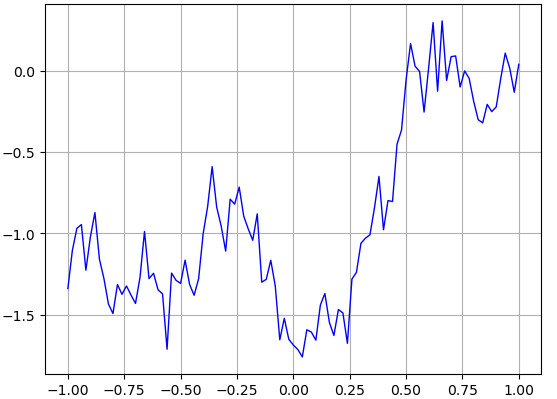
\includegraphics[scale=0.7]{images/gibbsRea.jpg}
\caption{Réalisation sur $[-1,1]$ par Galli-Gao-Gibbs}
\label{figGibbsRea}  
\end{center}
\end{figure}

\begin{remark}
  \label{nbIterationsMax}
  Dans OpenTURNS, l'algorithme se veut un peu différent en décidant pour une itération non pas de choisir un
  élément $a \in \llbracket 1;r \rrbracket $ selon une loi uniforme mais de tirer une permutation $\sigma$ de
  $\llbracket 1;r \rrbracket$ selon une loi uniforme puis de faire $r$ itérations où $a$ vaut d'abord $\sigma(1)$,
  puis $\sigma(2)$ jusqu'à $\sigma(r)$. Donc dans OpenTURNS, le nombre d'itérations $N_{it}$ mis en paramètre
  correspond dans les faits à $r \cdot N_{it} $ itérations où $r$ est la taille du vecteur gaussien à simuler.
\end{remark}

\section{Complexité algorithmique}
L'algorithme~\ref{algo5} admet une complexité en temps en
$O(Nr)$ et une complexité en mémoire en $O(r)$
(le stockage par des listes $z^n, z^c$ pour la simulation). Par
contre, pour l'algorithme~\ref{algo5} version OpenTURNS, en se fiant à la
remarque~\ref{nbIterationsMax}, bien que la complexité en mémoire reste inchangée,
la complexité en temps est en $O(N_{it}r^2)$ (pour une itération, lorsque $a$ parcourt
les valeurs de la permutation $\sigma$, $O(r)$ opérations
sont effectuées à chaque fois).

\section{Erreur et convergence numérique}
\label{gggErrConv}

\subsection{Dimension n=1}
Comme pour la méthode de Cholesky et celle des $\mathcal{H}$-matrices, pour simuler on a besoin 
d'un maillage $M$ et d'une fonction de covariance $C$ pour déduire $\Sigma$, la matrice de
covariance du problème $\Sigma$. Le choix des maillages et des fonctions de covariance sera celui
des maillages de la dimension $n=1$ évoqués pour la méthode de Cholesky (voir la sous-section~\ref{dimUnChol} du chapitre~\ref{chapCholesky})
et le nombre $m$ de n\oe uds dans les maillages ne variera plus entre $10$ et $10000$
mais plutôt entre $10$ et $100$ (pour des raisons de temps de calcul). Pour appliquer
la méthode de Galli-Gao-Gibbs, il faut aussi calibrer le nombre d'itérations $N_{it}$ évoqué à la
remarque~\ref{nbIterationsMax}. On décidera de le faire varier entre $10$ et $300$ pour les tests.


\subsection{Benckmarks}
\begin{table}[htbp]
  \centering
\begin{tabular}{|>{\centering\arraybackslash}p{1.5cm} |>{\centering\arraybackslash}p{1.6cm} |>{\centering\arraybackslash}p{1.0cm} |>{\centering\arraybackslash}p{2.0cm}|}
\hline
\small{Dimension } & \small{Nb de n\oe uds} & \small{$N_{it}$} & \small{Temps moyen d'une réalisation (en secondes)}\\
\hline
1 & 10 & 100 & 0.00637s    \\
\hline
1 & 10 & 200 & 0.01468s  \\
\hline
1 & 10 & 300 & 0.02217s   \\
\hline
\hline
1 & 100 & 100 & 0.15972s    \\
\hline
1 & 100 & 200 & 0.34042s    \\
\hline
1 & 100 & 300 & 0.47059s    \\
\hline
\end{tabular}
\end{table}

\begin{table}[htbp]
  \centering
\begin{tabular}{|c |c |c |c |c |}
\hline
Dimension & Nb de n\oe uds & $N_{it}$ & Nb de réalisations & erreur $L^2$ \\
\hline
1 & 10 & 10 & 250 & 0.18609  \\
\hline
1 & 10 & 10 & 500 & 0.11308   \\
\hline
1 & 10 & 10 & 750 & 0.07441  \\
\hline
1 & 10 & 10 & 1000 & 0.07942 \\
\hline
\hline
1 & 10 & 50 & 250 & 0.17034 \\
\hline
1 & 10 & 50 & 500 & 0.12572  \\
\hline
1 & 10 & 50 & 750 & 0.08582  \\
\hline
1 & 10 & 50 & 1000 & 0.08190 \\
\hline
\hline
1 & 10 & 100 & 250  & 0.14295 \\
\hline
1 & 10 & 100 & 500  & 0.10940 \\
\hline
1 & 10 & 100 & 750  & 0.09015  \\
\hline
1 & 10 & 100 & 1000 & 0.06226  \\
\hline
\hline
1 & 100 & 10 & 250 & 0.25851  \\
\hline
1 & 100 & 10 & 500 & 0.19295   \\
\hline
1 & 100 & 10 & 750 & 0.15731  \\
\hline
1 & 100 & 10 & 1000 & 0.13206 \\
\hline
\hline
1 & 100 & 50 & 250 & 0.27869 \\
\hline
1 & 100 & 50 & 500 & 0.18906  \\
\hline
1 & 100 & 50 & 750 &  0.16029 \\
\hline
1 & 100 & 50 & 1000 & 0.13728 \\
\hline
\hline
1 & 100 & 100 & 250  & 0.30028 \\
\hline
1 & 100 & 100 & 500  & 0.18475 \\
\hline
1 & 100 & 100 & 750  & 0.14346  \\
\hline
1 & 100 & 100 & 1000 & 0.13889  \\
\hline
\end{tabular}
\end{table}


%\chapter{Simulation par résolution d'un problème de Fredholm}

%chapitre méthode spectrale
\chapter{Simulation par méthode spectrale}

\label{spectralMeth}
La méthode qui va être présentée est fondée essentiellement sur un cours de l'école Polytechnique (voir~\cite{FogliCoursX}). Le lecteur
est invité à lire l'annexe~\ref{annexeA} afin de mieux saisir les objets mathématiques utilisés dans ce chapitre.\\


Soit $(\Omega, F, \mathbb{P})$ un espace probabilisé, $n$ et $d$ deux entiers naturels non nuls et
$X = (X_1, \dots, X_d) : \mathbb{R}^n \times \Omega \rightarrow \mathbb{R}^d$ un champ aléatoire gaussien centré,
continue en moyenne quadratique et faiblement stationnaire d'ordre 2, admettant pour mesure spectrale $M_X$.
On supposera que $M_X$ admet une densité spectrale $S_X: \mathbb{R}^n \rightarrow M_d(\mathbb{R})$.\\

On va chercher à simuler $X$ sur un domaine appelé le domaine de simulation $\overline{T} = \overline{T_1} \times \dots \times \overline{T_n} $
un pavé de $\mathbb{R}^n$ où $\overline{T_j} = [0,T_j], \; T_j \in \mathbb{R}^{*}_{+}$. Une fois ce domaine défini, on discrétisera $\overline{T}$ en
une famille finie de points et on simulera $X$ en ces points que l'on appellera les points de simulation. \uppercase{à} la fin, on obtiendra un champ aléatoire gaussien
discret qui approchera $X$ sur $\overline{T}$.


\section{Hypothèses sur la densité spectrale}

Commençons en imposant trois hypothèses sur la densité spectrale $S_X$. Les deux premières hypothèses permettront de justifier mathématiquement le choix de la discrétisation du domaine de
simulation et la dernière permettra de construire l'algorithme de simulation de la méthode spectrale.
\begin{hypothesis}
$S_X$ est à support compact dans le pavé $\overline{\Omega} = \overline{\Omega_{1}} \times \dots \times \overline{\Omega_{n}}$ où $\forall j \in \llbracket 1; n \rrbracket , \; \overline{\Omega_{j}} = [-\Omega_{cj},\Omega_{cj}], \; \Omega_{cj} \in \mathbb{R}^{*}_{+}$ \label{hyp1}
\end{hypothesis}

\begin{hypothesis}
  $tr(S_X)$ est bornée (où $tr: M_d(\mathbb{\mathbb{C}}) \rightarrow \mathbb{C}$ est la fonction trace) \label{hyp2} 
\end{hypothesis}

\begin{hypothesis}
$\forall \omega \in \overline{\Omega} \setminus \partial\overline{\Omega}, \; S(\omega)$ est de rang $d$ (donc $S(\omega)$ est hermitienne définie positive)
\end{hypothesis}


\noindent En général, $S_X$ n'est pas forcément à support compact. Néanmoins:
\begin{itemize}
\item $\forall t \in \mathbb{R}^n, \mathbb{E}(\|X(t)\|_{2}^{2}) = \int_{\mathbb{R}^n} tr(S_X(\omega)) d\omega < \infty$ 
\item en pratique, $S_X(\omega)$ tend rapidement vers $ 0_{M_d(\mathbb{R})}$ quand $\|\omega \| \rightarrow \infty$ \\
\end{itemize}

\noindent Dans ces conditions on peut espérer trouver, pour $\epsilon \in \mathbb{R}^{*}_{+}$, arbitrairement petit, un pavé pas trop large $\overline{\Omega^{\epsilon}} = \overline{\Omega_{1}^{\epsilon}} \times \dots \times \overline{\Omega_{n}^{\epsilon}}$ tel que:
\begin{itemize}
\item $\forall j \in \llbracket 1; n \rrbracket$, $\overline{\Omega_{j}^{\epsilon}} = [-\Omega_{cj}^{\epsilon},\Omega_{cj}^{\epsilon}], \; \Omega_{cj}^{\epsilon} \in \mathbb{R}^{*}_{+}$
\item $ \int_{\mathbb{R}^n \setminus \overline{\Omega^{\epsilon}}} tr(S_X(\omega)) d\omega \leq (\int_{\mathbb{R}^n} tr(S_X(\omega)) d\omega) \cdot \epsilon$\\
\end{itemize}

Dans une telle configuration, on serait alors tenté d'approcher $S_X$ par $\mathds{1}_{\overline{\Omega^{\epsilon}}}S_X$ pour $\epsilon$ assez petit. D'où l'idée de chercher non pas à simuler le champ aléatoire $X$ directement mais à l'approcher par le champ aléatoire $X^{\epsilon}$ d'ordre 2, à valeurs dans $\mathbb{R}^d$, centré, gaussien, continue en moyenne quadratique, faiblement stationnaire d'ordre 2 et de
densité spectrale $\mathds{1}_{\overline{\Omega^{\epsilon}}}S_X$ (l'existence d'un champ gaussien à valeurs dans $\mathbb{R}^d$ de densité spectrale $\mathds{1}_{\overline{\Omega^{\epsilon}}}S_X$ peut se justifier mais on n'insistera pas sur ce point).
On revient ainsi au cas de $S_X$ à support compact. 

%à modifier

\section{Factorisation de Cholesky} 
\label{choleskyFactSection}
Pour $\omega$ dans $\overline{\Omega} \setminus \partial\overline{\Omega}$, $S_X(\omega)$ est hermitienne définie positive, donc admet une décomposition de Cholesky 
$S_X(\omega)=\mathcal{H}(\omega)\mathcal{H}(\omega)^{*}$ où $\mathcal{H}(\omega)$ est une matrice triangulaire inférieure. 
Une décomposition (non unique) de Cholesky peut s'obtenir à l'aide la méthode de Cholesky généralisée aux matrices hermitiennes définies-positives.

\section{Subdivision du domaine spectral}
\label{subdivdomspec}
Soit $N_1, \dots, N_n$, $n$ entiers naturels non nuls.
Imposons d'abord un certain nombre de notations:

\begin{itemize}
\item $N = N_1 \times \dots \times N_n$

\item pour $j \in \llbracket 1; N \rrbracket, \; B_{N_j} = \llbracket 1; N_j \rrbracket$

\item $B_N = B_{N_1} \times \dots \times B_{N_n}$ (produit cartésien)\\
\end{itemize}

Une arête $[-\Omega_{cj},\Omega_{cj}]$ sera subdivisée en $N_j$ intervalles réguliers $M_{j,1},\dots , M_{j,N_j}$ de longueur
\begin{equation}
 \Delta\omega_{j} = \frac{2\Omega_{cj}}{N_j}
\end{equation}
et de centres respectifs $\omega_{j,1}, \dots, \omega_{j,N_j}$.\\
\newpage
\noindent D'où plus explicitement pour $j \in \llbracket 1; n \rrbracket,\; k_j \in B_{N_j}$:
\begin{itemize}
\item $\omega_{j,k_j} = -\Omega_{cj} + (k_j - \frac{1}{2})\Delta\omega_{j} = (2k_j - 1 - N_j)\frac{\Delta\omega_{j}}{2}$ 

\item $M_{j,k_j} = [\omega_{j,k_j} - \frac{\Delta\omega_{j}}{2}, \omega_{j,k_j} + \frac{\Delta\omega_{j}}{2}]$\\
\end{itemize}

On peut ainsi définir une subdivision régulière de $\overline{\Omega}$ en $N$ mailles \mbox{\og carrés \fg} $M_k$ de centre $\omega_k$ de la façon suivante. 
Pour $k = (k_1, \dots, k_n) \in B_N$:
\begin{equation}
M_k = M_{1,k_1} \times \dots \times M_{n,k_n} 
%\end{equation} 
%\begin{equation} 
\quad \text{et} \quad \omega_k = (\omega_{1,k_1}, \dots, \omega_{n,k_n}) \label{mailles}
\end{equation}


\begin{figure}[h]
\begin{center}
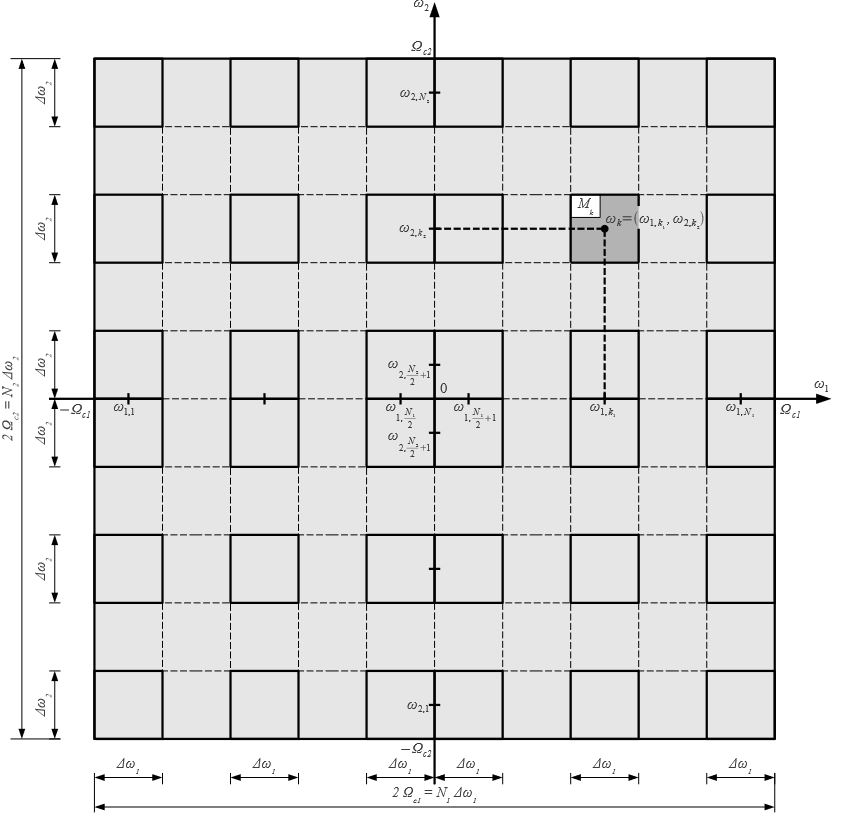
\includegraphics[scale=0.9]{images/grilleSpectraleDim2.jpg}
\caption{Subdivision du domaine spectral en dimension $n=2$}
\label{subdivSpecDim2}  
\end{center}
\end{figure}

\newpage
\begin{hypothesis}
  \label{symetrie} 
  Pour la suite, on supposera que les $N_j$ sont des multiples de 2. De cette façon, la subdivision $(M_k)_{k \in B_N}$ de $\overline{\Omega}$  est symétrique par rapport à l'origine (i.e si $\mathcal{S}$ est la symétrie de $\mathbb{R}^n$ qui à $x$ associe $-x$, alors $\mathcal{S}(\overline{\Omega}) = \overline{\Omega}$ et pour tout $k \in B_N$, il existe un unique $j \in B_N$ tel que $j \neq k$ et $\mathcal{S}(M_k) = M_j$ (on a même que $\omega_j = -\omega_k$)) et la famille des centres $(\omega_k)_{k \in B_N}$ ne contient pas l'origine $(0, \dots, 0)$. 
\end{hypothesis}




\section{Subdivision du domaine de simulation}
\label{subdiv}
On pose pour $j \in \llbracket 1; n \rrbracket, \; f_{max,j} = \frac{\Omega_{cj}}{2\pi}$. Il s'agit de la fréquence maximale sur l'arête spectrale $[-\Omega_{cj},\Omega_{cj}]$.\\

On obtient par le théorème d'échantillonage de Shannon, que pour $j \in \llbracket 1; n \rrbracket$ la fréquence d'échantillonage $f_{e,j}$ minimale requise pour représenter la densité spectrale $S_X$ sur le $j$\up{ème} axe de coordonnées vaut $2f_{max,j}$. Le pas d'échantillonage $\Delta t_{j}$ se définit alors ainsi:

\begin{equation} \forall j \in \llbracket 1; n \rrbracket , \; \Delta t_{j} = \frac{1}{f_{e,j}} = \frac{\pi}{\Omega_{cj}} \end{equation} 

\noindent On déduit alors la relation : pour $j \in \llbracket 1; n \rrbracket,\; \Delta t_{j}\Delta \omega_{j} = \frac{2\pi}{N_j}$.\\
Donc une fois que la discrétisation $(N_1, \dots, N_n)$ est donnée, le pas de pulsation $\Delta\omega_{j}$ et le pas de temps $\Delta t_{j}$ ne peuvent être choisis indépendamment.\\

Par ailleurs sous les hypothèses \ref{hyp1} et \ref{hyp2}, un théorème de Shannon plus fort garantit que la connaissance de $(X(k_1\Delta t_{1}, \dots, k_n\Delta t_{n}))_{(k_1, \dots, k_n) \in \mathbb{Z}^n}$ suffit pour déduire la loi du champ $X$ (voir page 446 de \cite{alma991000210539806616}). 

\noindent Par conséquent pour simuler un champ aléatoire approchant $X$, on pourra plutôt chercher à simuler un nombre fini de variables aléatoires de la famille $(X(k_1\Delta t_{1}, \dots, k_n\Delta t_{n}))_{(k_1, \dots, k_n) \in \mathbb{Z}^n}$. Explicitons lesquelles seront sélectionnées.\\

\noindent Posons pour $j \in \llbracket 1; n \rrbracket ,\; m_j \in \llbracket 1; N_j\rrbracket$:
\begin{itemize}
\item $t_{j,m_j} = (m_j - 1)\Delta t_{j}$
\item $T_j = N_j \Delta t_{j}$
\item $\overline{T_j} = [0, T_j]$


\item $\overline{T} = \overline{T_1} \times \dots \times \overline{T_n}$ (domaine de simulation)

\item pour $m \in B_N, t_m = (t_{1,m_1}, \dots, t_{n,m_n}) \in \overline{T}$ (points de simulation)\\
\end{itemize}

\begin{figure}[h]
\begin{center}
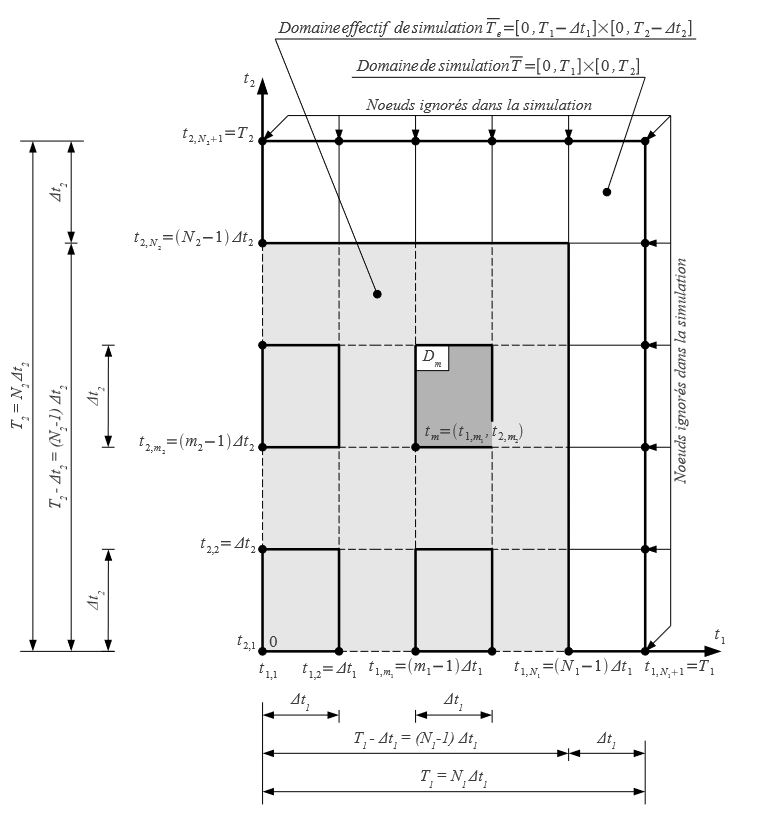
\includegraphics[scale=1.0]{images/MethSpect-domaineTemporelDeSimulationDim2.jpg}
\caption{Subdivision du domaine de simulation en dimension $n=2$}
\label{subdivSDomaineTempsDim2}  
\end{center}
\end{figure}

Avec ces notations, on peut maintenant dire que le but est de simuler la famille de vecteurs aléatoires $(X(t_m))_{m \in B_N}$ dont les éléments sont bien dans la
famille $(X(k_1\Delta t_{1}, \dots, k_n\Delta t_{n}))_{(k_1, \dots, k_n) \in \mathbb{Z}^n}$.


\section{Approximation du champ gaussien X}
\label{approxchmX}
$X$ est un champ d'ordre 2, centré, continue en moyenne quadratique et faiblement stationnaire d'ordre 2. On peut alors utiliser le théorème \ref{repSpec} de l'annexe \ref{annexeA}: on dispose de $\phi_X$, la mesure stochastique associée
à $X$ et issue de la mesure stochastique orthogonale centrée (m.s.o.c.) $I_X$
de mesure de base la mesure spectrale de $X$, $M_X$, telle que $\forall t \in \mathbb{R}^{n}$ :

\begin{equation}
X(t,.) = \displaystyle\int_{\mathbb{R}^n} \exp(i<t,\omega>_{n}) \phi_X(d\omega)= \displaystyle\int_{\overline{\Omega}} \exp(i<t,\omega>_{n}) \phi_X(d\omega) \label{specRepr}
\end{equation}

\begin{remark}
  La dernière égalité de la relation (\ref{specRepr}) se justifie par le support compact de $S_X$ dans $\overline{\Omega}$. En effet comme $M_X = S_X(\omega)d\omega$, on obtient que pour toute fonction $f$ dans $L^2(\mathbb{R}^n, M_X)$, $\|M_X\|$-presque partout, $f = \mathds{1}_{\overline{\Omega}} f$ (voir la définition~\ref{A22}). \\
\end{remark}

Or $\overline{\Omega}$ a été subdivisé par les mailles $M_k$ (voir la relation (\ref{mailles}))  et ces mailles sont à deux à deux disjointes (à un ensemble Lebesgue-négligeable près). D'où,
par linéarité de l'intégrale de Wiener et comme $X$ est à valeurs dans $\mathbb{R}^d$, pour $t \in \mathbb{R}^{n}$:
\begin{eqnarray}
X(t,.) &=& \displaystyle\sum_{k \in B_N} \displaystyle\int_{M_k} \exp(i<t,\omega>_{n}) \phi_X(d\omega) \notag{}\\
  &=& \mathfrak{Re}\biggl(\displaystyle\sum_{k \in B_N} \displaystyle\int_{M_k} exp(i<t,\omega>_{n}) \phi_X(d\omega)\biggr)
\end{eqnarray}

\`A partir de ce résultat, construisons peu à peu une approximation du processus $X$. On va d'abord faire l'approximation suivante:
~\\
\\$\forall t \in \mathbb{R}^{n}, \; \forall k \in B_N$,
\begin{eqnarray}
 \displaystyle\int_{M_k} \exp(i<t,\omega>_{n}) \phi_X(d\omega) &\approx& \displaystyle\int_{M_k} \exp(i<t,\omega_k>_{n}) \phi_X(d\omega) \notag{}\\
  &=& \exp(i<t,\omega_k>_{n}) \phi_X(M_k) 
\end{eqnarray}
\begin{remark}On peut y voir une quadrature par méthode du point milieu généralisée.\\\end{remark}

\noindent On obtient alors la première approximation de $X$ en posant pour $ t \in \mathbb{R}^{n}$: 

\begin{eqnarray}
Y(t,.) &=& \mathfrak{Re}\biggl(\displaystyle\sum_{k \in B_N} \exp(i<t,\omega_k>_{n}) \phi_X(M_k)\biggr) \notag{} \\
  &=& \mathfrak{Re}\biggl(I_X\biggl(\displaystyle\sum_{k \in B_N} \exp(i<t,\omega_k>_{n})\mathds{1}_{M_k}\biggl)\biggr) \notag{}
\end{eqnarray}

\noindent Pointons les propriétés suivantes (se justifiant à l'aide de la section~\ref{repSpecSect} de l'annexe \ref{annexeA}):
\begin{enumerate}
\item Comme $X$ est gaussien, les $\phi_X(M_k)$ sont des vecteurs gaussiens centrés de matrice de covariance complexe $\mathbb{E}(\phi_X(M_k)\phi_X(M_k)^{*}) = M_X(M_k) = \int_{M_k} S_X(\omega)d\omega$ 

\item Pour $(k,j) \in (B_N)^2,$ tel que $k \neq j,$ \\$  \; \mathbb{E}(\phi_X(M_k)\phi_X(M_j)^{*}) =  M_X(M_k \cap M_j) = 0_{M_d(\mathbb{C})}$.

\item Pour $(k,j) \in (B_N)^2, \; \mathbb{E}(\phi_X(M_k)\phi_X(M_j)^{\top}) = M_X(M_k \cap -(M_j))$

\item $Y$ est un champ gaussien centré \\
\end{enumerate}

\noindent Or par la symétrie de la subdivision $(M_k)_{k \in B_N}$ de $\overline{\Omega}$ (voir l'hypothèse~\ref{symetrie}), on a que pour tout $k \in B_N$, il existe un unique $j_k \in B_N$ différent de $k$ tel que $M_{j_k} = -M_k$. D'où:
\begin{equation}
  \label{five}
  \forall (k,l) \in (B_N)^2, \; \mathbb{E}(\phi_X(M_k)\phi_X(M_l)^{\top}) =
\begin{cases}
    M_X(M_k)    & \quad \text{si } l = j_k\\
    0_{M_d(\mathbb{C})}  & \quad \text{sinon }  \end{cases}
\end{equation}


\noindent $Y$ est un champ gaussien centré donc $Y$ est caractérisé par sa fonction de covariance que l'on note $C_Y: \mathbb{R}^n \times \mathbb{R}^n \rightarrow M_d(\mathbb{R})$. Par le calcul on obtient pour $(s,t) \in (\mathbb{R}^n)^2 :$
\begin{equation}
C_Y(s,t) = \mathbb{E}(Y(s)Y(t)^{\top}) = \mathfrak{Re}\biggl(\displaystyle\sum_{k \in B_N} e^{i<t-s,\omega_k>_n}M_X(M_k)\biggr)
\end{equation}

\noindent Ce résultat se fonde sur les propriétés 1, 2, 3, la formule~(\ref{five}) et sur la propriété suivante:
\begin{equation*}
\forall (A,B) \in M_{d,1}(\mathbb{C})^2, \; \mathfrak{Re}(A)\mathfrak{Re}(B)^{\top} = \frac{1}{2}(\mathfrak{Re}(AB^{\top}) + \mathfrak{Re}(AB^{*}))
\end{equation*}

\noindent Le souci devient alors les $(M_X(M_k))$ qui ont le défaut d'être définis par une intégrale. Cependant, en posant $\Delta\omega = \Delta\omega_1 \dots \Delta\omega_n$, on peut approcher les $M_X(M_k)$ ainsi: $ M_X(M_k) \approx \Delta\omega S_X(\omega_k)$ (encore une quadrature par méthode du point milieu généralisée).\\

On veut alors approcher le champ gaussien centré $Y$ par un champ gaussien centré dont la fonction de covariance vaut:
\begin{equation}
  K(s,t) = \Delta\omega \mathfrak{Re}\biggl(\displaystyle\sum_{k \in B_N} e^{i<t-s,\omega_k>_n}S_X(\omega_k)\biggr)
\end{equation}

 
\noindent Or on peut montrer que le champ $X_N$ suivant est à valeurs dans $\mathbb{R}^d$, gaussien, centré et que sa fonction de covariance vaut bien $K$:
\begin{equation}
  \forall t \in \mathbb{R}^n,\; X_N(t,.) = \mathfrak{Re}\biggl(\displaystyle\sum_{k \in B_N} \sqrt{\Delta\omega} \; e^{i<t,\omega_k>_{n}}\mathcal{H}(\omega_k)V_k \biggl) \label{formuleAppro}
\end{equation}
\noindent où:
\begin{itemize}
\item $\mathcal{H}(\omega)$ pour $\omega \in \overline{\Omega} \setminus \partial\overline{\Omega}$ a été définie plus tôt comme une factorisation de Cholesky (voir la section~\ref{choleskyFactSection})

\item les $(V_k)_{k \in B_N}$ sont des vecteurs gaussiens à valeurs dans $\mathbb{C}^d$ iid selon la loi normale centrée réduite complexe de $\mathbb{C}^d$ \\
\end{itemize}

\begin{remark}
  $\mathcal{H}(\omega_k)V_k $ est un produit matrice-vecteur
\end{remark}

\begin{remark}
\noindent $V$ un vecteur aléatoire à valeurs dans $\mathbb{C}^d$ suit la loi normale centrée réduite complexe si les parties réelle et imaginaire $\mathfrak{Re}(V)$ et $\mathfrak{Im}(V)$ suivent la loi normale centrée réduite de $\mathbb{R}^d$ et si $\mathfrak{Re}(V)$ et $\mathfrak{Im}(V)$ sont des vecteurs indépendants.
\end{remark}

Finalement on décide d'approcher le champ aléatoire $X$ par $X_N$ en les points de simulation $(t_m)_{m \in B_N}$ définis plus tôt (voir la section~\ref{subdiv}).
On cherche donc à simuler $(X_N(t_m,.))_{m \in B_N}$. Cette simulation est possible à l'aide d'un algorithme de simulation qui se déduit directement de la formule (\ref{formuleAppro}) du champ aléatoire $X_N$.

\section{Algorithme de simulation}

\subsection{Premier algorithme}
\label{firstone}
Pour modéliser les $(V_k)$ de la section précédente, il suffit de considérer $(U_{k,b,p})_{k \in B_N,  b \in \llbracket 0;1 \rrbracket, p \in \llbracket 1; d \rrbracket}$ une famille de $2\times Nd$ variables iid selon la loi normale centrée réduite de $\mathbb{R}$ et de poser pour $k \in B_N, V_k$ vecteur aléatoire à valeurs dans $\mathbb{C}^d$ tel que:
\begin{equation*}
  \mathfrak{Re}(V_k) = (U_{k,0,1}, \dots, U_{k,0,d}) \quad \text{et} \quad \mathfrak{Im}(V_k) = (U_{k,1,1}, \dots, U_{k,1,d})
\end{equation*}

\noindent On obtient alors l'algorithme de simulation suivant: 
\begin{itemize}
\item Soit $(u_{k,b,p})_{k \in B_N,  b \in \llbracket 0,1 \rrbracket, p \in \llbracket 1;d\rrbracket}$  une réalisation de taille $2\times Nd$ de la loi centrée réduite. 

\item On pose pour $k \in B_N, v_k \in \mathbb{C}^d$ tel que pour $p \in \llbracket 1;d\rrbracket$, la $p$-ième coordonnée de $v_k$ vaut $u_{k,0,p} + iu_{k,1,p}$

\item Pour $m \in B_N$ on pose:

   \begin{equation}x_N(t_m) = \mathfrak{Re}\biggl(\displaystyle\sum_{k \in B_N} \sqrt{\Delta\omega} \; e^{i<t_m,\omega_k>_{n}}\mathcal{H}(\omega_k)v_k \biggr) \label{formule1} \end{equation}

\end{itemize}


\noindent Les $x_N(t_m)$ constituent une réalisation du champ discret $(X_N(t_m))_{m \in B_N}$.


\subsection{Reformulation avec la densité spectrale fréquentielle}

Il est possible que l'on n'ait pas accès à la densité spectrale de $X$, $S_X$, mais à sa densité spectrale fréquentielle $S^{fr}_X$ (voir la sous-section~\ref{DSFr} de l'annexe~\ref{annexeA}). Dans ce cas, il est possible de reformuler l'algorithme de simulation en imposant quelques notations:\\

\begin{itemize}
\item  pour $k \in B_N, f_k = \frac{1}{2\pi} \cdot \omega_k \in \mathbb{R}^n \quad$ (fréquence associée aux $\omega_k$)
  
\item $\overline{D_f} = \frac{1}{2\pi}\overline{\Omega} = [-\frac{\Omega_{c1}}{2\pi},\frac{\Omega_{c1}}{2\pi}] \times \cdots \times [-\frac{\Omega_{cn}}{2\pi},\frac{\Omega_{cn}}{2\pi}]\quad$ (domaine fréquentiel)

\item $\forall j \in \llbracket 1; n \rrbracket, \; \Delta f_j = \frac{1}{2\pi}\Delta \omega_j $

\item $\Delta f = \Delta f_1 \dots \Delta f_n \in \mathbb{R}^{*}_{+}$ 

\item pour $f \in \overline{D_f} \setminus \partial \overline{D_f}, \; \tilde{H}(f) = (2\pi)^{\frac{n}{2}}\mathcal{H}(2\pi f) \quad$ ($2\pi f \in \overline{\Omega} \setminus \partial\overline{\Omega}$)\\

\end{itemize}

\noindent Remarquons d'abord que $\tilde{H}$ décrit une décomposition de Cholesky de $S^{fr}_X$:
\begin{equation*}
 \forall f \in \overline{D_f} \setminus \partial \overline{D_f}, \; \tilde{H}(f)\tilde{H}(f)^{*} = (2\pi)^{n}\mathcal{H}(2\pi f)\mathcal{H}(2\pi f)^{*} = (2\pi)^{n}S_X(2\pi f) = S^{fr}_X(f)
\end{equation*}

\noindent Une décomposition de Cholesky de $S^{fr}_X$ permet alors de réécrire les $x_N(t_m)$ introduits dans l'algorithme de simulation (voir la formule~(\ref{formule1})) à l'aide des notations posées juste avant:

\begin{equation*} \forall m \in B_N, \; x_N(t_m) = \mathfrak{Re}\biggl(\displaystyle\sum_{k \in B_N} \sqrt{\Delta f} \; e^{i<t_m,2\pi f_k>_{n}}\tilde{H}(f_k)v_k \biggl) \end{equation*}


\noindent Ce résultat indique la similitude des algorithmes de simulation peu importe si on voit le problème en fréquence ou en pulsation.


\subsection{Autre reformulation de l'approximation}

Dans l'annexe~\ref{annexeA}, on a exhibé multiples propriétés de la densité spectrale dont notamment celle-ci: $\forall \omega \in \mathbb{R}^n, \; S_X(-\omega) = \overline{S_X(\omega)}$. A partir de cette remarque, il est possible de décrire
un champ gaussien équivalent à $X_N$ (dans le sens où il suit la même loi que $X_N$).\\

\noindent Notons $A$ l'ensemble des $\omega_k$

\noindent Notons $B$ l'ensemble des $\omega_k$ tels que leur première coordonnée soit positive.

\noindent Notons $-B$ l'ensemble $\{ -b,\; b \in B\}$

\noindent On a supposé que les $(N_j)_{j \in \llbracket 1;n\rrbracket}$ étaient des multiples de $2$ (voir l'hypothèse~\ref{symetrie}). On a alors que $B$ est l'ensemble des $\omega_k$ tels que leur première coordonnée soit strictement positive. De façon plus explicite on a:
\begin{equation}
B = \{ \omega_k, \text{ où } k = (k_1, \dots, k_n) \in B_N \text{ et } k_1 \geq \frac{N_1}{2} + 1 \}
\end{equation}

\noindent Si on note  $\tilde{B} = \{ k = (k_1, \dots, k_n) \in B_N $ tel que $ k_1 \geq \frac{N_1}{2} + 1 \} $, on montre aussi que:
\begin{eqnarray*}
  A \setminus B &=& \{ \omega_{(N_1-k_1+1, N_2-k_2+1, \dots, N_n-k_n+1)} \text{ où } k = (k_1, \dots, k_n) \in \tilde{B} \}\\
  &=& \{ -\omega_k \text{ où } k = (k_1, \dots, k_n) \in \tilde{B} \}\\
  &=& -B
\end{eqnarray*}

\newpage
D'où le couple $(B,-B)$ forme une partition de $A$ l'ensemble des $\omega_k$. Il
est alors possible de réécrire la formule (\ref{formuleAppro}) du champ $X_N$. Si on pose pour $k = (k_1, \dots, k_n) \in B_N, \; j_k = (N_1-k_1+1, N_2-k_2+1, \dots, N_n-k_n+1)$,
alors pour $t \in \mathbb{R}^n$:

\begin{eqnarray*}
X_N(t, .) &=&  \mathfrak{Re}\biggl(\displaystyle\sum_{k \in B_N} \sqrt{\Delta\omega} \; e^{i<t,\omega_k>_{n}}\mathcal{H}(\omega_k)V_k\biggr) \\
&=& \mathfrak{Re}\biggl(\displaystyle\sum_{k = (k_1,\dots, k_n) \in \tilde{B}} \sqrt{\Delta\omega} \;( e^{i<t,\omega_k>_{n}}\mathcal{H}(\omega_k)V_k + e^{i<t,\omega_{j_k}>_{n}}\mathcal{H}(\omega_{j_k})V_{j_k}) \biggl) \\
&=& \mathfrak{Re}\biggl(\displaystyle\sum_{k = (k_1,\dots, k_n) \in \tilde{B}} \sqrt{\Delta\omega} \;( e^{i<t,\omega_k>_{n}}\mathcal{H}(\omega_k)V_k + e^{i<t,-\omega_k>_{n}}\overline{\mathcal{H}(\omega_k)}V_{j_k})\biggl) \\
&=& \mathfrak{Re}\biggl(\displaystyle\sum_{k = (k_1,\dots, k_n) \in \tilde{B}} \sqrt{\Delta\omega} \;( e^{i<t,\omega_k>_{n}}\mathcal{H}(\omega_k)V_k + \overline{e^{i<t,\omega_k>_{n}}\mathcal{H}(\omega_k)\overline{V_{j_k}}}) \biggl) \\
\end{eqnarray*}



\begin{remark}
  La notation $j_k$ est la définition explicite de la notation $j_k$ introduite à la section~\ref{approxchmX} et utilisée pour la formule~(\ref{five}).
\end{remark}


On observe que $\overline{V_{j_k}}$ suit la même loi que $V_{j_k}$ et plus généralement que la famille de vecteurs aléatoires composée de ceux de la famille $(V_k)_{k \in \tilde{B}}$ et de ceux de la famille $(\overline{V_{j_k}})_{k \in \tilde{B}}$ forme une famille de variables aléatoires iid qui peut être confondue avec la famille $(V_k)_{k \in B_N}$. Donc si on pose pour $t \in \mathbb{R}^n$:

\footnotesize{
\begin{equation}
\tilde{X}_N(t, .) =  \mathfrak{Re}\biggl(\displaystyle\sum_{k = (k_1,\dots, k_n) \in \tilde{B}} \sqrt{\Delta\omega} \;( e^{i<t,\omega_k>_{n}}\mathcal{H}(\omega_k)V_k + \overline{e^{i<t,\omega_k>_{n}}\mathcal{H}(\omega_k)V_{j_k}}) \biggr)\\
\end{equation}
}

\normalsize{
  \noindent alors ce champ $\tilde{X}_N$ suit la même loi que le champ $X_N$. Par conséquent, en raisonnant comme à la sous-section~\ref{firstone}, on peut en déduire sans souci un deuxième algorithme
  pour simuler les $(\tilde{X}_N(t_m))_{m \in B_N}$. L'avantage de ce nouvel algorithme sera de diminuer les calculs. En effet la connaissance des $(\mathcal{H}(\omega_k))_{k \in \tilde{B}}$, qui s'obtiennent
  par la méthode de Cholesky, suffit. D'où 2 fois moins de calculs ($\tilde{B}$ est de cardinal $N/2$).}


\section{Algorithme de simulation et TFD}

Si on reconsidère dans la sous-section~\ref{firstone}, la formule~(\ref{formule1}) des $x_N(t_m)$ qui décrit le premier algorithme de simulation, la formule se veut sous une forme
matricielle très condensée. De plus cette formule n'utilise pas la définition des $t_m$ et des $\omega_k$ (voir les sections~\ref{subdivdomspec} et~\ref{subdiv})
. Il est donc intéressant de développer la formule des $x_N(t_m)$ pour chaque coordonnée $p$ allant de $1$ à $d$ (que l'on va noter $x_{N,p}(t_m)$)
Dans cette section, on met en avant la présence d'une transformée de
Fourier discrète (TFD), dont l'algorithme associé se veut particulièrement efficace.\\


\noindent Pour $m \in B_N$ et $k \in B_N$, on obtient en développant le produit scalaire suivant:
\begin{eqnarray*}
  <t_m,\omega_k>_{n} \; &=&  \; \displaystyle\sum_{j = 1}^{n} t_{j,m_j} \omega_{j,k_j} \\ 
  &=& \; \displaystyle\sum_{j = 1}^{n} \biggl( -\frac{\pi (m_j - 1)(N_j - 1)}{N_j} + \frac{2\pi(m_j - 1)(k_j -1)}{N_j} \biggr)
\end{eqnarray*}
 
~\\
\noindent Si on utilise cette formule dans la formule des $x_N(t_m)$, on obtient alors pour $m \in B_N$ et $p \in \llbracket 1;d \rrbracket$ :

\begin{equation*}
  x_{N,p}(t_m) = \sqrt{\Delta \omega} \; \mathfrak{Re} \biggl (y_{N,p}(m) \cdot \exp \biggl(-i \pi \displaystyle\sum_{j = 1}^{n} \frac{(m_j - 1)(N_j - 1)}{N_j} \biggr) \biggr)  
\end{equation*}

\noindent où:
\begin{itemize}

\item $y_{N,p}(m) = \displaystyle\sum_{k \in B_N}  z_{p}(k) \cdot \exp \biggl(2i\pi \displaystyle\sum_{j = 1}^{n} \frac{(m_j - 1)(k_j -1)}{N_j} \biggr)$\\
~\\
\item $z_{p}(k) \; = \; \displaystyle\sum_{q = 1}^{d} \mathcal{H}_{pq}(\omega_k) \cdot (u_{k,0,q} + i.u_{k,1,q}) \;$ pour $k \in B_N$\\
\end{itemize}
~\\
On observe pour $p \in \llbracket 1;d \rrbracket$ que la famille $(y_{N,p}(m))_{m \in B_N}$ n'est rien d'autre que
la transformée de Fourier discrète (TFD) de la famille $(z_{p}(k))_{k \in B_N}$.\\
De façon générale si $n \in \llbracket 1;3 \rrbracket$, l'algorithme de simulation admet une complexité en temps en $O(d Nlog(N)+d^3 N)$ à cause 
des $d$ TFDs et du calcul des factorisations de Cholesky. Comme $d$ varie en général entre $1$ et $3$
on peut parler d'une complexité en $O(Nlog(N))$). La complexité en mémoire est en  $O(d^2 N)$, en raison du
stockage des $N$ factorisations de Cholesky. 


\section{Propriétés des approximations $X_N$}

Dans cette section, on répertorie un ensemble de propriétés vérifiées
par l'approximation du champ gaussien $X$, $X_N$, introduit à la section~\ref{approxchmX} par la formule~\ref{formuleAppro}.\\

\begin{itemize}
  \item $X_N$ est un champ gaussien centré, homogène tel que:
   \begin{equation}
    \mathbb{E}(\|X_N\|_{2}^{2}) \; = \; \Delta \omega \cdot \displaystyle\sum_{k \in B_N} tr(S_X(\omega_k))    
   \end{equation}

 \item Si on note $R_{X_N}$ sa fonction d'autocovariance qui à $s \in \mathbb{R}^n$ associe $\mathbb{E}(X_N(0)X_N(s))^{T}$, alors:
   \begin{equation}
    R_{X_N}(s) = \Delta\omega \cdot \mathfrak{Re}\biggl (\displaystyle\sum_{k \in B_N} e^{i<s,\omega_k>_n}S_X(\omega_k)\biggr)  \label{autocov}  
   \end{equation}

   \noindent On remarque que $\displaystyle\sum_{k \in B_N} e^{i<s,\omega_k>_n}S_X(\omega_k)$ est un réel \\

 \item $X_N$ est continue en moyenne quadratique et admet une mesure spectrale $M_{X_N}$ à valeurs dans $M_d(\mathbb{R})$ tel que:
   \begin{equation}
     M_{X_N} = \Delta\omega \cdot \displaystyle\sum_{k \in B_N} S_X(\omega_k)\delta_{\omega_k} \label{mesSpec}
   \end{equation}
   où $\delta_{\omega_k}$ est la mesure de Dirac en $\omega_k$ (mesure sur $(\mathbb{R}^n,\mathcal{B}(\mathbb{R}^n)$)\\

 \item $X_N$ est presque sûrement à trajectoires continues.\\

 \item Les trajectoires de $X_N$ sont de période $\tau = (\tau_1, \cdots, \tau_n)$\\
   où $\forall j \in \llbracket 1;n \rrbracket, \; \tau_j = \frac{4\pi}{\Delta \omega_j} = 2T_j$
   (i.e $\forall j \in \llbracket 1;n \rrbracket, \; \forall t \in \mathbb{R}^n, \; \\ X_N(t_1, \cdots, t_j + \tau_j, \cdots, t_n) = X_N(t_1, \cdots, t_j, \cdots, t_n)$)
\end{itemize}
~\\

Considérons maintenant une suite $( N^{j} = (N_1^{j}, \cdots, N_n^{j}))_{j \in \mathbb{N}}$ à valeurs dans $\mathbb{N}^n$. Pour $j \in \mathbb{N}$, on note $N_{inf}^{j} = \displaystyle\inf_{i \in \llbracket 1;n \rrbracket} N_i^{j}$. On suppose que $N_{inf}^{j} \underset{j \to \infty}{\to} \infty$.\\

\noindent Notons maintenant pour $j \in \mathbb{N}$,  $X_{N^j}$ le champ aléatoire défini par la formule~(\ref{formuleAppro}), $M_{X_{N^{j}}}$ sa mesure spectrale définie par
la formule~\ref{mesSpec} et $R_{X_{N^{j}}}$ la fonction d'autocovariance de $X_{N^j}$ définie par la formule~(\ref{autocov})
où dans les formules la discrétisation $(N_1, \cdots, N_n)$ qui définit les $\omega_k$
est remplacée par la discrétisation $(N_1^{j}, \cdots, N_n^{j})$.\\

\noindent On obtient alors des propriétés de convergence:\\


\begin{itemize}
\item La suite $(X_{N^j})_{j \in \mathbb{N}}$ converge en loi vers le champ aléatoire $X$.
\item La suite $(R_{N^j})_{j \in \mathbb{N}}$ converge uniformément dans tout compact de $\mathbb{R}^n$ vers $R_X$ la fonction d'autocovariance de $X$.
\item Pour tout $(k,l) \in \llbracket 1;d \rrbracket^2$, la suite de mesures complexes $((M_{N^j})_{k,l})_{j \in \mathbb{N}}$ converge étroitement vers la mesure $(M_X)_{k,l}$ 
\item Si $S_X$ est de classe $C^1$ (resp. $C^2$) sur $\overline{\Omega}$, alors la vitesse des 2 convergences précédentes est en $(N_{inf}^{j})^{-1}$ (resp. $(N_{inf}^{j})^{-2}$).
\end{itemize}

\section{Erreur et convergence numérique}
\label{erreurConvSpectral}
\subsection{Nouvel estimateur}

Dans le cas de la méthode spectrale, on ne choisira pas d'estimer
l'erreur $L^2$ de $N$ réalisations (voir la sous-section~\ref{quantifErreur}
du chapitre \ref{chapCholesky}) afin de valider cette méthode
de simulation. On rappelle que l'erreur $L^2$ permet de voir à quel point
par $N$ réalisations, on approche la matrice de covariance $\Sigma$ du problème. Or
même si à partir d'une densité spectrale on peut obtenir par calcul la fonction
d'autocovariance d'un processus (et donc la fonction de covariance dont on déduit la matrice $\Sigma$), on
peut être dans une situation où seule l'information de la densité spectrale
est disponible. C'est donc cette dernière que l'on cherchera à estimer à
l'aide de $L$ réalisations indépendantes du même processus sur le domaine
de simulation. Explicitons l'estimateur évoqué dans la référence~\cite{FogliCoursX}.\\

Soit $(x^{(1)}(t_m))_{m \in B_N}, \cdots, (x^{(L)}(t_m))_{m \in B_N} $ $L$ réalisations indépendantes du
processus $X_N$ (voir la formule (\ref{formuleAppro}) de la section~\ref{approxchmX}) en les points de simulation $(t_m)_{m \in B_N}$ (voir
la section~\ref{subdiv}). Pour valider nos simulations, on décide d'utiliser plus précisement un estimateur de la densité spectrale fréquentielle $S_X^{fr}$ en les
points $(f_k)_{k \in B_N}=(\frac{1}{2\pi}\omega_k)_{k \in B_N}$ (voir formule~(\ref{mailles}) de la section~\ref{subdivdomspec}) que l'on qualifiera de points fréquentiels associés aux points de simulation.
On définit alors pour $k = (k_1, \cdots, k_n) \in B_N$ l'estimateur de $S_X^{fr}(f_k)$ :
\begin{equation}
\hat{S}(f_k) = \frac{1}{L} \displaystyle\sum_{l = 1}^{L} \hat{Z}^{(l)}(k)\hat{Z}^{(l)}(k)^{*} \in M_d(\mathbb{C})  
\end{equation}

où:

\begin{itemize}

\item pour $l \in \llbracket 1;L \rrbracket$, $\hat{Z}^{(l)}(k) = (\hat{Z}^{(l)}_{1}(k), \cdots, \hat{Z}^{(l)}_{d}(k))^{T}$\\
  
\item pour $l \in \llbracket 1;L \rrbracket$, pour $p \in \llbracket 1;d \rrbracket$:
  \begin{equation*} \hat{Z}^{(l)}_{p}(k) = \displaystyle\sum_{m \in B_N} Z_{p}^{(l)}(m)\cdot\exp \biggl(-2i\pi \displaystyle\sum_{j = 1}^{n} \frac{(m_j -1)(k_j -1)}{N_j} \biggr)  \end{equation*}

\item pour $l \in \llbracket 1;L \rrbracket$, $m \in B_N $ et  $p \in \llbracket 1;d \rrbracket$:
  \begin{equation*} Z^{(l)}_{p}(m) = \Delta t \cdot W_{\bar{T}}(t_m) \cdot x^{(l)}_{p}(t_m) \cdot \exp \biggl (i\pi \displaystyle\sum_{j = 1}^{n} \frac{(m_j -1)(N_j -1)}{N_j} \biggr)  \end{equation*}

\item pour $s \in \mathbb{R}^{n}, W_{\bar{T}}(s) = W_{T_1}(s_1) \cdots W_{T_n}(s_n)$ (on parle de fenêtre temporelle de dimension $n$ sur $\bar{T} = [0,T_1] \times \cdots \times [0,T_n]$) \\

\item pour $s \in \mathbb{R}$ et $j \in \llbracket 1;n \rrbracket$, $W_{T_j}(s) = \frac{1}{\sqrt{T_j}} W(\frac{s}{T_j})$ où
$W$ est une fenêtre temporelle de dimension $1$ standard.
\end{itemize}

\begin{definition}
  Une fenêtre temporelle d'énergie normalisée standard ou juste fenêtre temporelle de dimension $1$ standard est une fonction $W: \mathbb{R} \rightarrow \mathbb{R}$ mesurable telle que:
\begin{itemize}
\item $supp(W) \subset [0,1]$ (support de $W$ inclus dans $[0,1]$)
\item $W(1-t) = W(t)$ pour $t \in \mathbb{R}$
\item $\displaystyle\int_{\mathbb{R}} W(t)^2 dt = \displaystyle\int_{0}^{1} W(t)^2 dt = 1$
\item si on note $\hat{W}$ la transformée de Fourier de $W$
et que l'on note pour $T \in \mathbb{R}^{*}_{+}$ et $\omega \in \mathbb{R}$, $G_{T}(\omega) = \frac{T}{2\pi} |\hat{W}(T\omega)|^{2}$, alors
quand $T$ tend vers l'infini, $G_T$ converge en distribution vers la masse de Dirac en $0$.
\end{itemize}
\end{definition}

\begin{remark}
  $\hat{W}(\omega) = \displaystyle\int_{\mathbb{R}} e^{-i\omega t} W(t) dt $
\end{remark}
%~\\
\begin{remark}
  Pour $T \in \mathbb{R}^{*}_{+}$, $W_{T}: t \rightarrow \frac{1}{\sqrt{T}} W(\frac{t}{T}) $ est appelé fenêtre temporelle et
  vérifie les propriétés suivantes:
  \begin{itemize}
   \item $supp(W_T) \subset [0,T]$ 
   \item $W_T(T-t) = W_{T}(t)$ pour $t \in \mathbb{R}$
   \item $\displaystyle\int_{\mathbb{R}} W_T(t)^2 dt = \displaystyle\int_{0}^{T} W_T(t)^2 dt = 1$
   \item $\frac{1}{2\pi} |\hat{W_T}(\omega)|^{2} = G_{T}(\omega)$ pour $\omega \in \mathbb{R}$
     (on dit alors que $G_{T}$ est la fenêtre spectrale associée à $W_{T}$)
\end{itemize}
\end{remark}

\noindent Dans la référence~\cite{alma991000210539806616}, plus de détails sur les fenêtres temporelles sont évoqués
et leur rôle est d'essayer d'améliorer les estimations d'une densité spectrale. On peut citer comme exemple de
fenêtre temporelle standard, la fenêtre de Hamming que l'on utilisera pour nos tests numériques et qui est
définie de la façon suivante pour $t \in \mathbb{R}$:

\begin{equation} W(t) = 1.5863 \;(0.54 - 0.46\cos(2\pi t))\;\mathds{1}_{[0,1]}(t) \end{equation}

Dans les références~\cite{FogliCoursX} et~\cite{alma991000210539806616} , la pertinence (dans le cas des champs gaussiens surtout)
d'utiliser un tel estimateur pour la densité spectrale $S_X^{fr}$ en augmentant le nombre de réalisations $L$
y est un peu plus développé mais on n'entrera pas dans les détails.\\

Finalement on quantifie l'erreur de simulation en définissant l'erreur absolue $\epsilon$ suivante:
\begin{equation}  \epsilon = \max_{k \in B_N} \|\hat{S}(f_k) - S_X^{fr}(f_k)\|_{F}  \label{errAbs}\end{equation}

\subsection{Résultats numériques}

Dans l'annexe~\ref{codeNumAnnexe}, dans la section~\ref{dossSpec}, plusieurs
densités spectrales y sont évoquées et ont une notation: \eqref{S1} et sa fonction d'autocovariance associée \eqref{R1}, \eqref{S2}
et sa fonction d'autocovariance associée \eqref{R2}, etc... On utilisera cette notation afin de les désigner par la suite.
Par ailleurs  on maintient toujours les notations utilisées jusqu'à maintenant pour décrire la
méthode spectrale: $N_1, \cdots, N_n, f_{max,1}, \cdots, f_{max,n}$ et ainsi de suite. Pour nos tests, $n \in \llbracket 1;3 \rrbracket$ et
bien qu'il ne soit pas nécessaire d'associer un maillage aux points de simulation, en raison de la répartition régulière dans l'espace
des points de simulation, on peut y associer tout de même un maillage
triangulaire dont les n\oe uds sont les points de simulations et dont les $n$-simplexes sont définis de la même façon que pour les maillages
évoqués à la section~\ref{errConvCholesky} du chapitre~\ref{chapCholesky}.\\


Les sous-sous-sections suivantes décrivent les différents tests numériques effectués. Ces derniers sont contenus dans le fichier spectral.py (voir la section~\ref{dossSpec} de
l'annexe~\ref{codeNumAnnexe}). Pour tester l'estimateur de densité spectrale, il a fallu choisir le nombre de réalisations indépendantes $L$
du processus $X_N$ et on l'a fait varier entre $100$ et $2000$. L'erreur de simulation sera l'erreur absolue $\epsilon$
décrite par la formule~\eqref{errAbs}. Pour le choix de la fenêtre temporelle
standard, on opte pour la fenêtre de Hamming.

\subsubsection{Dimension n=1}
En dimension 1, on a choisi la densité spectrale (fréquentielle)~\eqref{S1} où le paramètre $A$ a été
fixé à 5.0. Comme la densité~\eqref{S1} est à support dans $[-A,A]$, il est pertinent de choisir $f_{max,1} = A$.
Le nombre de points de simulation $N = N_1$ varie entre $10$ et $10000$. La connaissance de $N$ et $f_{max,1}$ permet
de déduire les $N$ points de simulation $(\frac{m-1}{2f_{max,1}})_{m \in \llbracket 1;N \rrbracket}$. Le point de simulation de valeur maximale est
donc le point $t_{N} = \frac{N-1}{2f_{max,1}}$, qui est le temps effectif de simulation en constraste avec le temps de simulation
$T_1 = \frac{N}{2f_{max,1}}$. Aux points de simulation, on associe les points fréquentiels:
\begin{equation*} \biggl((2i -1 - N) \frac{f_{max,1}}{N_1}\biggr)_{i \in \llbracket 1;N \rrbracket} \end{equation*}

\subsubsection{Dimension n=2}
En dimension 2, on a choisi la densité spectrale~\eqref{S4} où le paramètre $\sigma$ vaut $1$ et les paramètres $b_1$ et $b_2$ ont été
fixés respectivement à $1$ et $4$. On a fixé $f_{max,1} = \frac{20}{2\pi}$ et  $f_{max,2} = \frac{5}{2\pi}$.
Le nombre de points de simulation $N = N_1 \times N_2$ varie entre $10$ et $10000$ et $N_1 = N_2$. La connaissance de $N$, $f_{max,1}$ et $f_{max,2}$  permet
de déduire les $N$ points de simulation: \begin{equation*} \biggl(\biggl(\frac{i-1}{2f_{max,1}},\frac{j-1}{2f_{max,2}}\biggr)\biggr)_{(i,j) \in \llbracket 1;N_1 \rrbracket \times \llbracket 1;N_2 \rrbracket } \end{equation*}
auxquels on associe les points fréquentiels:
\begin{equation*} \biggl(\biggl((2i -1 - N_1) \frac{f_{max,1}}{N_1}, (2j -1 - N_1) \frac{f_{max,2}}{N_2}\biggr)\biggr)_{(i,j) \in \llbracket 1;N_1 \rrbracket \times \llbracket 1;N_2 \rrbracket } \end{equation*}

\subsubsection{Dimension n=3}
En dimension 3, on a choisi la densité spectrale~\eqref{S3} où le paramètre $a$ a été fixé à $1.0$. Les fréquences maximales
$f_{max,1}, f_{max,2}, f_{max,3}$ ont été fixées toutes trois à $10$.
Le nombre de points de simulation $N = N_1 \times N_2 \times N_3$ varie entre $10$ et $10000$ et  $N_1 = N_2 = N_3 $. La connaissance de $N$, $f_{max,1}$, $f_{max,2}$ et $f_{max,3}$ permet
de déduire les $N$ points de simulation:
\begin{equation*} \biggl (\biggl(\frac{i-1}{2f_{max,1}},\frac{j-1}{2f_{max,2}},\frac{k-1}{2f_{max,3}}\biggr)\biggr)_{(i,j,k) \in \llbracket 1;N_1 \rrbracket \times \llbracket 1;N_2 \rrbracket \times \llbracket 1;N_3 \rrbracket} \end{equation*} 
auquels on associe les points fréquentiels:
\small{
\begin{equation*}  \biggl(\biggl((2i -1 - N_1) \frac{f_{max,1}}{N_1}, (2j -1 - N_1) \frac{f_{max,2}}{N_2},(2k -1 - N_1) \frac{f_{max,3}}{N_3}\biggr)\biggr)_{(i,j,k) \in \llbracket 1;N_1 \rrbracket \times \llbracket 1;N_2 \rrbracket \times \llbracket 1;N_3 \rrbracket} \end{equation*}
}

\normalsize{}

\subsubsection{Benchmarks}

\phantom{
\noindent espace\\
espace\\
}

\begin{table}[htbp]
  \centering
\begin{tabular}{|>{\centering\arraybackslash}p{1.7cm} |>{\centering\arraybackslash}p{1cm} |>{\centering\arraybackslash}p{7cm} |}
\hline
Dimension & Nb de n\oe uds $N$ & Temps moyen d'une réalisation (en seconde) \\
\hline
1 & 10 & 0.00024s    \\
\hline
1 & 100 & 0.00196s  \\
\hline
1 & 1000 & 0.01924s   \\
\hline
1 & 10000 & 0.19921s    \\
\hline
\hline
2 & 16 & 0.00060s    \\
\hline
2 & 100 & 0.00271s    \\
\hline
2 & 1024 & 0.02546s  \\
\hline
2 & 10000 & 0.24736s   \\
\hline
\hline
3 & 8 & 0.00040s    \\
\hline
3 & 64 & 0.00200s    \\
\hline
3 & 1000 & 0.02714s    \\
\hline
3 & 10648 & 0.27015s  \\
\hline
\end{tabular}
\end{table}

\begin{table}[htbp]
  \centering
\begin{tabular}{|c |c |c |c |c |}
\hline
Dimension & Nb de n\oe uds $N$  & Nb de réalisations $L$ & erreur $\epsilon$ \\
\hline
1 & 100 & 100 & 0.02323   \\
\hline
1 & 100 & 500 & 0.00803    \\
\hline
1 & 100 & 1000 & 0.00968    \\
\hline
1 & 100 & 2000 & 0.00485    \\
\hline
\hline
1 & 500 & 100 & 0.02758    \\
\hline
1 & 500 & 500 & 0.01412  \\
\hline
1 & 500 & 1000 & 0.00815    \\
\hline
1 & 500 & 2000 & 0.00835    \\
\hline
\hline
1 & 1000 & 100 & 0.03043    \\
\hline
1 & 1000 & 500 & 0.01536    \\
\hline
1 & 1000 & 1000 & 0.01083   \\
\hline
1 & 1000 & 2000 & 0.00751    \\
\hline
\hline
\hline
2 & 100 & 100 & 0.56987   \\
\hline
2 & 100 & 500 & 0.39173    \\
\hline
2 & 100 & 1000 & 0.42713    \\
\hline
2 & 100 & 2000 & 0.45083    \\
\hline
\hline
2 & 484 & 100 & 5.07162    \\
\hline
2 & 484 & 500 & 2.54857   \\
\hline
2 & 484 & 1000 & 2.94699    \\
\hline
2 & 484 & 2000 & 3.13654  \\
\hline
\hline
2 & 1024 & 100 & 2.01205    \\
\hline
2 & 1024 & 500 & 1.83634    \\
\hline
2 & 1024 & 1000 & 0.93156    \\
\hline
2 & 1024 & 2000 & 1.05494    \\
\hline
\hline
\hline
3 & 64 & 100 & 1.80454.$10^{-5}$   \\
\hline
3 & 64 & 500 & 1.66974.$10^{-5}$    \\
\hline
3 & 64 & 1000 & 1.62478.$10^{-5}$    \\
\hline
3 & 64 & 2000 & 1.52534.$10^{-5}$    \\
\hline
\hline
3 & 512 & 100 & 0.00027    \\
\hline
3 & 512 & 500 & 0.00024   \\
\hline
3 & 512 & 1000 & 0.00021    \\
\hline
3 & 512 & 2000 & 0.00022    \\
\hline
\hline
3 & 1000 & 100 & 0.00065    \\
\hline
3 & 1000 & 500 & 0.00062    \\
\hline
3 & 1000 & 1000 & 0.00054    \\
\hline
3 & 1000 & 2000 & 0.00057    \\
\hline
\end{tabular}
\end{table}
\newpage


\begin{remark}
  Dans le tableau de l'erreur $\epsilon$, l'erreur ne décroît pas forcément bien vers $0$ et certains niveaux d'erreur
  sont étonnamment élevés (dimension 2). On soupçonne un bug qui est toujours en cours d'investigation au moment de la
  rédaction du rapport.
\end{remark}

\phantom{oyez}\\
\phantom{oyez}\\

\begin{figure}[h]
\centering
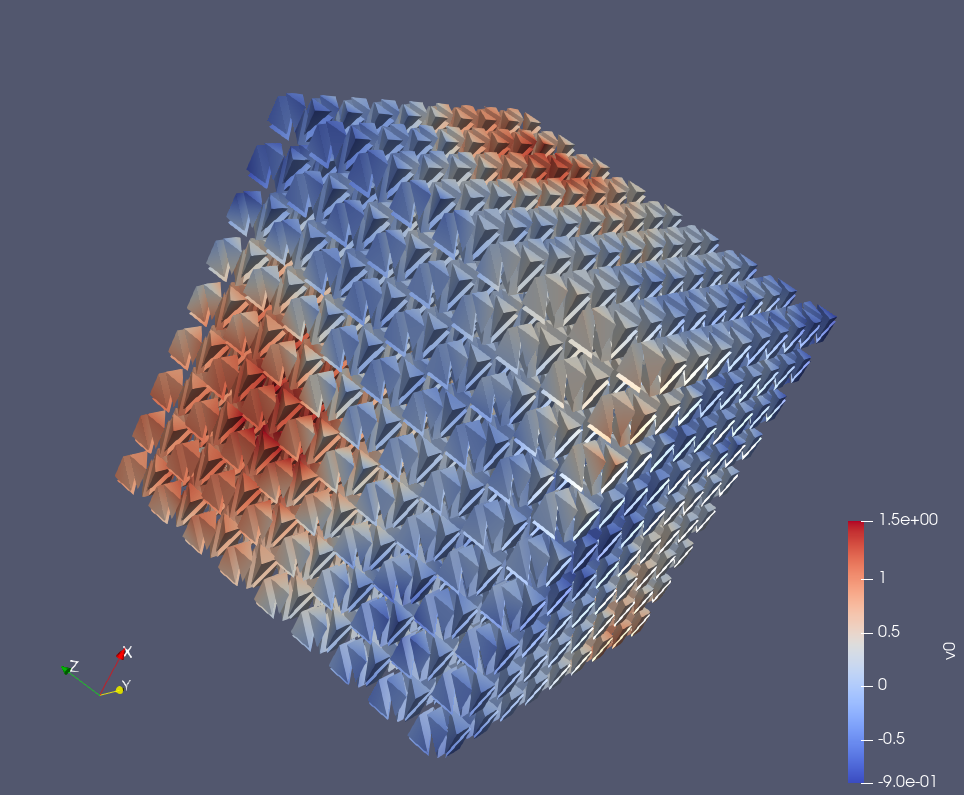
\includegraphics[scale=0.4]{images/meshSpectral3D-1000.png}
\caption{Réalisation en dimension 3 où $N = 1000$ }
\label{ReaDim2-961}  

\end{figure}


%chapitre interpolation P1
\chapter{Simulation par $\mathbb{P}_{1}$-interpolation}
\label{P1Interpol}
Supposons pouvoir simuler un champ gaussien $X$
sur les n\oe uds d'un maillage $M$ décrivant la fermeture d'un ouvert borné $D$.
Par une interpolation $\mathbb{P}_1$, il est possible à partir de toutes les réalisations du processus
$X$ connu en les n\oe uds de $M$, d'obtenir un nouveau processus $\tilde{X}$
sur $\bar{D}$. On aimerait que le processus $\tilde{X}$ devienne une bonne
approximation du processus $X$ (pour un maillage $M$ suffisamment raffiné)
en les n\oe uds d'un nouveau maillage $M'$ inclus dans $\bar{D}$.\\

L'intérêt pratique de la $\mathbb{P}_{1}$-interpolation est que certaines méthodes de simulation
sont très efficaces sur des maillages $M$ comme les maillages
semblables à ceux de la méthode spectrale du chapitre précédent ou
comme les maillages ne présentant pas une concentration de n\oe uds
(efficacité de la compression en $\mathcal{H}$-matrice). D'où l'idée
de transférer par $\mathbb{P}_{1}$-interpolation sur
le maillage d'intérêt $M'$, les résultats d'une simulation efficace
sur $M$.\\

\section{Cadre théorique}
\label{theory}
\noindent Soit $(\Omega,\mathcal{F},\mathbb{P})$ un espace probabilisé \\
Soit $n,d$ deux entiers naturels non nuls et $D$ un ouvert borné de $\mathbb{R}^n$  \\
On note $\lambda^n$ la mesure de Lebesgue sur $D$\\
On admet aussi que $D$ peut être décrit par un maillage triangulaire.

%Soit $X=(X_t)_{t\in \mathbb{R}^n}$ un processus gaussien centré d'ordre 2 à valeurs dans $\mathbb{R}^d$ \\
%Notons $C: \mathbb{R}^n \times \mathbb{R}^n \rightarrow M_d(\mathbb{R}) $ la fonction de covariance de $X$ \\
%Soit $M$ une triangulation de $D$ et on note $(n_i)_{i \in \{1,m\}}$ les n\oe uds
%du maillage $M$.


\begin{definition}
\label{RFmesurable}On dit que le champ aléatoire $X : D \times \Omega \rightarrow \mathbb{R}^d$ est un
champ aléatoire mesurable si $X$ est une fonction mesurable, où $D \times \Omega$
a été muni de la tribu issue de la complétion de la mesure-produit $\lambda^n \otimes \mathbb{P}$ 
\end{definition}

En se référant à \cite{ScheuererMichael2010Rots}, on obtient que tout champ aléatoire $X$ d'ordre 2 dont
les éléments diagonaux de la fonction de covariance sont des fonctions continues
admet une version $Y$ qui est mesurable. Par conséquent, pour qu'un champ
gaussien puisse être considéré comme un champ aléatoire mesurable, il suffit de
supposer que les éléments diagonaux de sa fonction de covariance soient des
fonctions continues.
~\\

Pour étudier les champs aléatoires mesurables, on introduit également l'espace de Hilbert
$(L^2_{\mathbb{R}^d}(D \times \Omega, \lambda^n \otimes \mathbb{P}),\|\cdot\|)$,  l'ensemble des fonctions $\phi$ de $D \times \Omega$ dans
$\mathbb{R}^d$ telles que:
~\\
\begin{itemize}
\item $\phi$ est $(\mathcal{B}(D) \otimes \mathcal{F},\mathcal{B}(\mathbb{R}^d))$-mesurable
\item la quantité
$\|\phi\|^2 = \mathbb{E}(\displaystyle\int_D \|\phi(t,.)\|_2^2 \ud \lambda^n(t))$ est finie
\end{itemize}
~\\
\noindent Ainsi, un champ aléatoire mesurable $X$ est dans
$L^2_{\mathbb{R}^d}(D \times \Omega , \lambda^n \otimes \mathbb{P}) $ si et seulement si $\|X\|$ est une quantité finie.


\section{Approximation d'une fonction par méthode des éléments finis $\mathbb{P}_1$}

L'approximation $\mathbb{P}_1$-Lagrange est une manière très classique en analyse numérique d'approcher la
solution d'une EDP (équation aux dérivées partielles). Par conséquent, tout lecteur qui souhaitera des détails
sur ce procédé pourra se référer au livre de Grégoire Allaire \cite{alma991003727179806616}. De ce livre, on utilise
notamment les définitions de maillage triangulaire ou triangulation (page 175) et de suite de maillages réguliers (page 188).\\
~\\
Rappelons rapidement en quoi consiste l'approximation d'une fonction par la méthode des éléments finis.
On considère un maillage triangulaire $M$ décrivant la fermeture de $D$ ($D$ peut être supposé connexe). Si on note $(n_i)_{i \in \llbracket 1,m \rrbracket}$  les n\oe uds de $M$, on dispose
d'un unique $m$-uplet $(\psi_1, \cdots, \psi_m)$ de fonctions continues de $\bar{D}$ dans $\mathbb{R}$ et polynomiales de degre $1$ sur
chaque $n$-simplexe du maillage $M$ et tel que:
\begin{equation*}
  \forall (i,j) \in \llbracket 1,m \rrbracket^2, \psi_i(n_j) = \delta_{i,j}
\end{equation*}

\begin{remark}
On appelle les $\psi_i$, les fonctions de base du maillage $M$ 
\end{remark}

On définit alors pour $f: \bar{D} \rightarrow \mathbb{R}^d$ une fonction continue sur $D$, $R_{M,d}(f)$, l'interpolée $\mathbb{P}_1$ de $f$
comme la fonction telle que:
\begin{equation}
  \label{ContiInterpol}
  \forall t \in \bar{D}, \; R_{M,d}(f)(t) = \displaystyle\sum_{i=1}^m \psi_i (t)\cdot f(n_i)
\end{equation}

\begin{remark}
  $R_{M,d}(f)$ prend les mêmes valeurs que $f$ en les n\oe uds du maillage
\end{remark}
~\\
L'opérateur d'interpolation $R_{M,d}$ décrit l'approximation par interpolation $\mathbb{P}_1$-Lagrange des fonctions continues sur $\bar{D}$.
Dans le livre de Grégoire Allaire, tout est présenté dans le cas où $d = 1$, notamment les espaces de Sobolev qui seront utiles
pour faire des estimations. Cependant, il n'est guère difficile de généraliser la définition des espaces de Sobolev dans le cas $d > 1$ comme il va suivre.

\section{Espaces de Sobolev et interpolation}

On suppose que le lecteur est familier avec les espaces de Sobolev
notés $W^{k,p}(O)$ ou $H^{k}(O)$, où $O$ est un ouvert. On peut ainsi présenter une légère généralisation des espaces de Sobolev où
les (classes de) fonctions sont à valeurs dans $\mathbb{R}^d$, où $d$ est
éventuellement strictement supérieur à 1.

\begin{definition}
Pour $O$ un ouvert de $\mathbb{R}^n$, pour $k \in \mathbb{N}^{*}$ et $p \in [1,\infty]$:
\begin{equation*}
  W^{k,p}_{\mathbb{R}^d}(O) = \{ f = (f_1, \cdots, f_d)^{T}: O \rightarrow \mathbb{R}^d \; /\; \forall i \in \llbracket 1,d \rrbracket, \; f_i \in W^{k,p}(O) \}\\
\end{equation*}
\end{definition}
\noindent On se servira par la suite surtout de cet ensemble:
\begin{equation*}
  H^{k}_{\mathbb{R}^d}(O) = W^{k,2}_{\mathbb{R}^d}(O)
\end{equation*}

\begin{property}
  Pour $k \in \mathbb{N}^{*}$, l'espace $H^{k}_{\mathbb{R}^d}(O)$ est un espace de
  Hilbert s'il est muni de la norme
  \smash{\mbox{$\|\cdot \|_{H^{k}_{\mathbb{R}^d}(O)}$}} telle que pour
  $f \in H^{k}_{\mathbb{R}^d}(O)$:
  \begin{equation*} \|f\|_{H^{k}_{\mathbb{R}^d}(O)}^2 = \displaystyle\sum_{i = 1}^d \|f_i\|_{H^{k}(O)}^2  \end{equation*}
\end{property}
~\\
Avec ces définitions, notons les 2 propriétés suivantes:

\begin{property}
Pour tout maillage triangulaire $M$ de $\bar{D}$ et toute fonction continue $f: \bar{D} \rightarrow \mathbb{R}^d, \;R_{M,d}(f) \in H^{1}_{\mathbb{R}^d}(D)$
\end{property}

\begin{property}[Injection de Sobolev]
Soit $k \in \mathbb{N}$ tel que $k+1 > n/2$.\\$\forall w \in H^{k+1}_{\mathbb{R}^d}(D)$, $w$ est la restriction sur $D$ d'une fonction continue sur $\bar{D}$.
\end{property}

On est maintenant apte à introduire un théorème majeur pour la suite ainsi que son corollaire. Considérons $(\mathcal{T}_h)_{h \in \mathbb{R}^{*}_{+}}$ une suite de maillages (triangulaires) réguliers de $\bar{D}$. On rappelle que le paramètre $h$ désigne le maximum des diamètres des $n$-simplexes qui composent le maillage $\mathcal{T}_h$.
Pour $h \in \mathbb{R}^{*}_{+}$, on note $R_{h,d}$ l'opérateur d'interpolation $R_{\mathcal{T}_h,d}$. 

\begin{theorem}
  Soit $k \in \mathbb{N}$ tel que $k+1 > n/2$. Il existe $C \in \mathbb{R}^{*}_{+}$ tel que:
  \begin{equation*}
    \forall h \in  \mathbb{R}^{*}_{+}, \forall v \in H^{k+1}(D), \;
    \|v - R_{h,1}(v) \|_{H^{1}(D)} \leq C h^k \|v\|_{H^{k+1}(D)}
  \end{equation*}
\end{theorem}

\begin{corollary}
  \label{ineqInterpol}
  Soit $k \in \mathbb{N}$ tel que $k+1 > n/2$. Il existe $C \in \mathbb{R}^{*}_{+}$ tel que:
  \begin{equation*}
    \forall h \in  \mathbb{R}^{*}_{+}, \forall v \in H^{k+1}_{\mathbb{R}^d}(D), \;
    \|v - R_{h,d}(v) \|_{H^{1}_{\mathbb{R}^d}(D)} \leq C h^k \|v\|_{H^{k+1}_{\mathbb{R}^d}(D)}
  \end{equation*}
\end{corollary}


\section{Espaces de Sobolev et champs aléatoires}

Lorsque l'on étudie les réalisations d'un champ aléatoire, on peut s'interroger
sur la régularité des trajectoires (continuité, différentiabilité). Dans cette
section, on exhibe des conditions pour qu'un champ aléatoire mesurable (voir
la définition~\ref{RFmesurable}) puisse admettre presque sûrement que des
trajectoires dans un espace de Sobolev. Tout ce qui suit est fondé en grande partie sur
le livre de Hristopulos \cite{alma991004158221006616}, l'article de Scheuerer \cite{ScheuererMichael2010Rots} et le chapitre 4 de \textit{``The Theory of Stochastic Processes I''}~\cite{GihmanSkoro}. 


\subsection{Sur la différentiabilité en moyenne quadratique d'un champ aléatoire}

\`A la page 183 dans \cite{alma991004158221006616}, pour $X: D \times \Omega \rightarrow \mathbb{R}$
un champ aléatoire d'ordre 2 et $i \in \llbracket 1;n \rrbracket$, on définit, si elle existe,
la dérivée partielle de $X$ en moyenne
quadratique par rapport à la $i$\up{ème} variable que l'on note $\frac{\partial}{\partial x_i} X$ ou $\frac{\partial X}{\partial x_i}$. On remarque que sa définition ne
revient qu'à dire que l'application $\gamma: D \rightarrow L^2(\Omega,\mathbb{P})$
qui à $t \in D$ associe $\gamma(t) = X(t,.)$ admet une dérivée
partielle par rapport à la $i$\up{ème} variable sur $D$.\\
~\\
On peut alors définir, si elles existent, les dérivées partielles en moyenne quadratique sur $D$ d'ordre supérieur à 1 de
$X$, $\frac{\partial^{k}}{\partial x_{\alpha_1} \cdots \partial x_{\alpha_k} } X$ où $\alpha_1, \cdots , \alpha_k$ sont $k$ entiers entre $1$ et $n$ et où la notation indique qu'on a dérivé par rapport à
la $\alpha_k$\up{ème} variable (en moyenne quadratique) , puis par rapport à la $\alpha_{k-1}$\up{ème} variable, ainsi de suite et à la fin par rapport à la $\alpha_{1}$\up{ème} variable. On dira alors que $\frac{\partial^{k}}{\partial x_{\alpha_1} \cdots \partial x_{\alpha_k} } X$  est une dérivée partielle (en moyenne quadratique) de $X$ d'ordre $k$.

~\\On s'apprête à mettre en avant une condition suffisante pour qu'un champ aléatoire d'ordre 2 et centré admette des dérivées partielles en moyenne quadratique. Mais il
faut d'abord introduire le concept de dérivée généralisée mixte. Considérons \mbox{$X: D \times \Omega \rightarrow \mathbb{R}$} un champ
aléatoire d'ordre 2, centré et dont on note la fonction de covariance
$C: D \times D \rightarrow \mathbb{R}$

\begin{definition}
  Soit $i \in \llbracket 1;n \rrbracket$ et $(s,t) \in D \times D $. On note $e_i$ le
  $i$\up{ème} vecteur de la base canonique de $\mathbb{R}^n$.\\

  On dit alors que $C$ admet une dérivée mixte généralisée en $(s,t)$ par
  rapport à la $i$\up{ème} variable si
  \begin{equation}
    \lim_{(h,k) \to (0,0)} \frac{C(s+h\cdot e_i\;,\;t+k\cdot e_i)-C(s,\;t+k\cdot e_i)-C(s+h\cdot e_i \;,t)+C(s,t)}{hk}
  \end{equation}
  existe. Si tel est le cas, on notera cette limite $(D^{i,i}C)(s,t)$.\\
\end{definition}

\begin{remark}
  On peut voir $D^{i,i}$ comme un opérateur ayant pour ensemble de départ et d'arrivée l'ensemble des fonctions allant de $D \times D$ dans $\mathbb{R}$
\end{remark}

\begin{theorem}
  Pour $i \in \llbracket 1;n \rrbracket$, $X$ admet une dérivée partielle en moyenne quadratique par rapport
  à la $i$\up{ème} variable si et seulement $\forall t \in D$, $(D^{i,i}C)(t,t)$ existe et est fini. \\

  \noindent Si tel est le cas, alors $\forall (s,t) \in D \times D$, $(D^{i,i}C)(s,t)$ existe et est finie. De plus:
  \begin{equation} \mathbb{E}\biggl(\frac{\partial X}{\partial x_i} (s) \frac{\partial X}{\partial x_i} (t)\biggl) = (D^{i,i}C)(s,t) \end{equation}
\end{theorem}

\begin{remark}
  Ce théorème explicite donc la fonction de covariance de $\frac{\partial X}{\partial x_i}$.
\end{remark}

\begin{definition}
\noindent Soit $\alpha_1, \cdots , \alpha_k$ $k$ entiers entre $1$ et $n$.\\
\begin{itemize}  
\item On définit $D^{(\alpha_1, \alpha_1), \cdots, (\alpha_k, \alpha_k)}$ comme l'opérateur $D^{\alpha_1, \alpha_1} \circ \cdots \circ D^{\alpha_k, \alpha_k}$.\\

\item Soit $\kappa \in \mathbb{N}^n$ tel que $\forall i \in \llbracket 1;n \rrbracket$, $\kappa_i$ indique
  le nombre d'éléments parmi les $k$ entiers $\alpha_1, \cdots , \alpha_k$ qui prennent la valeur $i$.\\
  
\noindent Alors si pour tout permutation de $\llbracket 1;k \rrbracket$, $D^{(\alpha_{\sigma(1)}, \alpha_{\sigma(1)}), \cdots, (\alpha_{\sigma(k)}, \alpha_{\sigma(k)})}C$
  est bien défini sur $D \times D$ et que $D^{(\alpha_{\sigma(1)}, \alpha_{\sigma(1)}), \cdots, (\alpha_{\sigma(k)}, \alpha_{\sigma(k)})}C = \\D^{(\alpha_1, \alpha_1), \cdots, (\alpha_k, \alpha_k)}C$,
  alors on définit $D^{\kappa}C$ comme étant la fonction \\$D^{(\alpha_1, \alpha_1), \cdots, (\alpha_k, \alpha_k)}C$.
\end{itemize}
\end{definition}


\begin{corollary}
Soit $\alpha_1, \cdots , \alpha_k$ $k$ entiers entre $1$ et $n$, $(s,t) \in D \times D $.\\
\noindent La dérivée partielle en moyenne quadratique $\frac{\partial^{k}}{\partial x_{\alpha_1} \cdots \partial x_{\alpha_k} } X$ existe si et seulement si $\forall t \in D$, la quantité $(D^{(\alpha_1, \alpha_1), \cdots, (\alpha_k, \alpha_k)}C)(t,t)$ est bien définie et finie.\\

\noindent Si tel est le cas, alors $\forall (s,t) \in D \times D$, $(D^{(\alpha_1, \alpha_1), \cdots, (\alpha_k, \alpha_k)}C)(s,t)$ est défini et fini. De plus:
  \begin{equation} \mathbb{E}\biggl(\frac{\partial^{k}X}{\partial x_{\alpha_1} \cdots \partial x_{\alpha_n} } (s) \frac{\partial^{k}X}{\partial x_{\alpha_1} \cdots \partial x_{\alpha_n} }(t)\biggl) = (D^{(\alpha_1, \alpha_1), \cdots, (\alpha_k, \alpha_k)}C)(s,t) \end{equation}
\end{corollary}
~\\
\begin{property}
Soit $(s,t) \in D \times D $ et $m \in \mathbb{N}$.\\
\noindent Si $C$ est une fonction de classe $\mathcal{C}^{2m}$ sur $D \times D$ alors $\forall \kappa \in \mathbb{N}^d$ tel que $|\kappa| \leq m$,
$D^{\kappa}C$ est bien définie sur $D \times D$ et $\forall (s,t) \in D \times D$:
\begin{equation}
  (D^{\kappa}C)(s,t)= \frac{\partial^{2|\kappa|}}{\partial s_1^{\kappa_1} \cdots \partial s_n^{\kappa_n} \partial t_1^{\kappa_1} \cdots \partial t_n^{\kappa_n}} (s,t)
\end{equation}
\end{property}

\subsection{Résultat de régularité des trajectoires}

On dédie cette sous-section à un autre résultat important qui permet de déduire une estimation théorique en lien avec la simulation d'un processus gaussien par méthode de $\mathbb{P}_1$-interpolation présentée à la section suivante. Ce résultat est tiré de l'article de Scheuerer \cite{ScheuererMichael2010Rots}. \`A partir de la preuve
évoquée dans l'article, il est possible de raffiner un peu plus le propos, ce
qui s'avèrera nécessaire pour justifier des propriétés mathématiques de la future méthode.

\begin{theorem}
  Soit $O$ un ouvert de $\mathbb{R}^n$, $X: O \times \Omega \rightarrow \mathbb{R}$ un champ aléatoire
  mesurable dont on note $C: O \times O \rightarrow \mathbb{R}$ la fonction
  de covariance. Soit $k \in \mathbb{N}^{*}$.\\
\noindent Alors si pour tout
  $\alpha \in \mathbb{N}^{n}$ tel que $|\alpha| \leq k$, $D^{\alpha}C$ existe
  sur $O \times O$ et est continue sur la diagonale de $O \times O$, alors
  les trajectoires de $X$ sont presque sûrement dans $H_{loc}^{k}(O)$ et pour
  tout $\alpha \in \mathbb{N}^{n}$ tel que $|\alpha| \leq k$, $\mathbb{P}(\omega)-$presque sûrement, la dérivée en moyenne quadratique $\frac{\partial^{|\alpha|}}{\partial x_{1}^{\alpha_1} \cdots \partial x_{n}^{\alpha_n} } X(.,\omega)$ coincide presque partout (pour la mesure de Lebesgue dans $O$) avec la dérivée faible d'indice $\alpha$ de $X(.,\omega), \; \partial^{\alpha} X(.,\omega)$.\\
~\\  
  Si de plus pour tout $\alpha \in \mathbb{N}^{n}$ tel que $|\alpha| \leq k$:
  \begin{equation}
  \displaystyle\int_O D^{\alpha}C(t,t) dt < +\infty
  \end{equation}

\noindent Alors on a même que les trajectoires de $X$ sont presque sûrement dans $H^{k}(O)$ (ce qui revient à dire que pour tout $\alpha \in \mathbb{N}^{n}$,
  $\mathbb{P}(\omega)-$presque sûrement $\partial^{\alpha} X(.,\omega)$ est dans $L^2(O)$).
\end{theorem}

\begin{corollary}
  \label{RFcorollary}
Soit $O$ un ouvert de $\mathbb{R}^n$, $X = (X_1, \cdots, X_d): O \times \Omega \rightarrow \mathbb{R}^d$ un champ aléatoire
  mesurable dont on note $C = (C_{i,j}): O \times O \rightarrow M_d(\mathbb{R})$ la fonction
  de covariance. Soit $k \in \mathbb{N}^{*}$.\\
\noindent Si pour tout $i \in \llbracket 1;d \rrbracket$,
  $\alpha \in \mathbb{N}^{n}$ tel que $|\alpha| \leq k$, $D^{\alpha}C_{i,i}$ existe
sur $O \times O$, est continue sur la diagonale de $O \times O$, et que
\begin{equation}
\displaystyle\int_O D^{\alpha}C_{i,i}(t,t) dt < +\infty
\end{equation}
alors
  les trajectoires de $X$ sont presque sûrement dans $H_{\mathbb{R}^d}^{k}(O)$ et pour \\$i \in \llbracket 1;d \rrbracket$ et $\alpha \in \mathbb{N}^{n}$ tel que $|\alpha| \leq k$, $\mathbb{P}(\omega)-$presque sûrement, la dérivée en moyenne quadratique $\frac{\partial^{|\alpha|}}{\partial x_{1}^{\alpha_1} \cdots \partial x_{n}^{\alpha_n} } X_i(.,\omega)$ coincide dans $L^2(O)$ avec la dérivée faible d'indice $\alpha$ de $X_i(.,\omega), \; \partial^{\alpha} X_i(.,\omega)$.
\end{corollary}

Avec ce théorème, nous avons tous les outils nécessaires pour justifier les
propriétés théoriques de la méthode de simulation par $\mathbb{P}_1$-interpolation.

\section{Méthode de $\mathbb{P}_1$-interpolation}

\subsection{Description de la méthode}

Considérons $X: \bar{D} \times \Omega \rightarrow \mathbb{R}^d$ un champ
aléatoire mesurable gaussien centré dont on note
$C: \bar{D} \times \bar{D} \rightarrow M_d(\mathbb{R})$ la fonction de
covariance. Soit $M$ un maillage triangulaire de $\bar{D}$ dont on note $(n_i)_{i \in \llbracket 1;m \rrbracket}$ les $m$ n\oe uds du maillage $M$. On note $(\psi_i)_{i \in \llbracket 1;m \rrbracket}$ les fonctions de base du maillage $M$.\\

\noindent On définit alors l'interpolée $\mathbb{P}_1$ de $X$ (par le maillage $M$), le processus
$\mathcal{R}_{M,d}X$ définit de la fonction suivante: 

\begin{equation}
  \label{RFInterpol}
  \forall (t,\omega) \in \bar{D} \times \Omega, \; (\mathcal{R}_{M,d}X)(t,\omega) =  \displaystyle\sum_{i=1}^m \psi_i (t)\cdot X(n_i,\omega)
\end{equation}

\noindent On appellera l'opérateur $\mathcal{R}_{M,d}$, l'opérateur d'interpolation $\mathbb{P}_1$ (qu'on applique ici à des champs aléatoires à valeurs dans $\mathbb{R}^d$).
\begin{remark}
Comme $X$ est un champ gaussien, il s'avère que $\mathcal{R}_{M,d}X$ est aussi un champ gaussien.
\end{remark}

\` A partir de ce nouveau processus, si on dispose de $M'$ un maillage qui décrit la fermeture d'un ouvert inclus dans $D$, on désire étudier le
processus $\mathcal{R}_{M,d}X$ en les n\oe uds du maillage $M'$ en se demandant s'il
approche bien le processus $X$ en les points du maillage $M'$. La prochaine sous-section donne un début d'élément de réponse en exhibant
une forme de convergence mais cette convergence ne dit aucunement qu'en raffinant le maillage $M$ alors l'interpolée converge en loi en
les n\oe uds du maillage $M'$ vers le processus $X$.\\

Par ailleurs, une telle méthode suppose que l'on sait simuler $X$ en les n\oe uds de $M$. Donc la complexité en temps et en mémoire
de l'algorithme associé à la méthode dépend du choix de simulation de $X$ en les n\oe uds de $M$. Néanmoins une fois qu'on connaît
en les n\oe uds $(n_i)_{i \in \llbracket 1;m \rrbracket}$ les valeurs $X(n_i,\omega)$, la $\mathbb{P}_1$-interpolation qui donne
en les n\oe uds $(\tilde{n_{i}})_{i \in \llbracket 1;\tilde{m} \rrbracket}$ de $M'$ les $(\mathcal{R}_{M,d}X)(\tilde{n_{i}},\omega)$, admet une complexité algorithmique indépendante
du choix de simulation. Sur OpenTURNS, l'implémentation des maillages de dimension $n$ allant de $1$ à $3$ à l'aide
d'une structure hiérarchique de données de type k-d tree permet d'accélérer la $\mathbb{P}_1$-interpolation. Sans entrer
dans les détails, si on suppose que $d \leq 3$ et que tous les maillages $M$ et $M'$ étudiés admettent une borne uniforme sur le
nombre de $n$-simplexes partageant un même n\oe ud, alors la complexité temporelle de la $\mathbb{P}_1$-interpolation
est en $O(\tilde{m}.log(m))$. Sous ces mêmes hypothèses, on obtient une complexité mémoire en $O(m+\tilde{m})$.


\subsection{Estimation d'erreur}

Le théorème suivant donne un cadre pertinent quant à l'utilisation de la méthode de $\mathbb{P}_1$-interpolation.
Considérons d'abord $(\mathcal{T}_h)_{h \in \mathbb{R}^{*}_{+}}$ une suite de maillages réguliers de $\bar{D}$
dont on note $\mathcal{R}_{h,d}$ leur opérateur d'interpolation $\mathbb{P}_1$
de champs aléatoires à valeurs dans $\mathbb{R}^d$ défini par la formule~(\ref{RFInterpol}) et $R_{h,d}$  leur opérateur d'interpolation $\mathbb{P}_1$ de fonctions continues de $\bar{D}$ dans $\mathbb{R}^d$ défini par la formule~(\ref{ContiInterpol}) pour le maillage $\mathcal{T}_h$.

\begin{theorem}
\label{EstimeeTheo}
Soit $k \in \mathbb{N}$ tel que $k+1 > n/2$. Si pour tout $i \in \llbracket 1;d \rrbracket$, $\alpha \in \mathbb{N}^{n}$ tel que $|\alpha| \leq k+1$, $D^{\alpha}C_{i,i}$ existe
sur $D \times D$, est continue sur la diagonale de $D \times D$, et tel que
\begin{equation}
\displaystyle\int_D D^{\alpha}C_{i,i}(t,t) dt < +\infty
\end{equation}

\noindent alors $X$ admet presque sûrement des trajectoires dans $H^{k+1}_{\mathbb{R}^d}(D)$ (donc des trajectoires continues sur $\bar{D}$) et il existe une constante $K \in \mathbb{R}_{+}$ tel que $\forall h \in \mathbb{R}_{+}^{*}$:

\begin{equation}
\|X - \mathcal{R}_{h,d}X \| \leq K \cdot h^{k} 
\end{equation}
\end{theorem}

\begin{remark}
$\| \cdot \|$ est la norme définie à la fin de la section~\ref{theory}.
\end{remark}

\begin{remark}
  Ce résultat ne nécessite pas que $X$ soit un champ gaussien. Le résultat
  reste donc valide sans cette hypothèse.
\end{remark}

\begin{proof}
  En utilisant le corollaire~\ref{RFcorollary}, on obtient que les trajectoires
  de $X$ sont presque sûrement dans $H^{k+1}_{\mathbb{R}^d}(D)$ et que $\mathbb{P}(\omega)$-presque sûrement,
  pour tout $i \in \llbracket 1;d \rrbracket$ et $\alpha \in \mathbb{N}^{n}$ tel que $|\alpha| \leq k+1$,
  $\frac{\partial^{|\alpha|}}{\partial x_{1}^{\alpha_1} \cdots \partial x_{n}^{\alpha_n} } X_i(.,\omega) = \partial^{\alpha}X_i(.,\omega)$ dans $L^2(D,\lambda^n)$.
  Donc par le corollaire~\ref{ineqInterpol}, on dispose de $L \in \mathbb{R}_{+}^{*}$ tel que,
  $\mathbb{P}(\omega)$-presque sûrement, pour tout $h \in \mathbb{R}^{*}_{+}$:
  \begin{eqnarray*}
    \|X(.,\omega) - \mathcal{R}_{h,d}(X(.,\omega)) \|_{H^{1}_{\mathbb{R}^d}(D)}^2 &=& \|X(.,\omega) - R_{h,d}(X(.,\omega)) \|_{H^{1}_{\mathbb{R}^d}(D)}^2 \\
    &\leq& L^2 \cdot h^{2k} \cdot \|X(.,\omega)\|_{H^{k+1}_{\mathbb{R}^d}(D)}^2
  \end{eqnarray*}

  \noindent De plus $\mathbb{P}(\omega)$-presque sûrement:
  \begin{eqnarray*}
    \|X(.,\omega)\|_{H^{k+1}_{\mathbb{R}^d}(D)}^2 &=& \displaystyle\sum_{i=1}^{d}  \displaystyle\sum_{\substack{\alpha \in \mathbb{N}^n \\ |\alpha| \leq k+1}} \int_D |\partial^{\alpha}X_i(t,\omega)|^2 dt \\
                                          &=& \displaystyle\sum_{i=1}^{d}  \displaystyle\sum_{\substack{\alpha \in \mathbb{N}^n \\  |\alpha| \leq k+1} } \int_D |\frac{\partial^{|\alpha|}}{\partial x_{1}^{\alpha_1} \cdots \partial x_{n}^{\alpha_n} } X_i(.,\omega)|^2 dt
  \end{eqnarray*}

  \noindent Donc par passage à l'espérance, pour tout $h \in \mathbb{R}^{*}_{+}$:
\footnotesize{
  \begin{eqnarray*}
    \mathbb{E}(\|X(.,\omega) - \mathcal{R}_{h,d}(X(.,\omega)) \|_{H^{1}_{\mathbb{R}^d}(D)}^2) &\leq& L^2 \cdot h^{2k} \cdot \displaystyle\sum_{i=1}^{d} \; \mathbb{E}(\|X(.,\omega)\|_{H^{k+1}_{\mathbb{R}^d}(D)}^2) \\
    &=& L^2 \cdot h^{2k} \cdot \displaystyle\sum_{i=1}^{d} \displaystyle\sum_{\substack{\alpha \in \mathbb{N}^n \\  |\alpha| \leq k+1} } \mathbb{E}\biggl(\int_D |\frac{\partial^{|\alpha|}}{\partial x_{1}^{\alpha_1} \cdots \partial x_{n}^{\alpha_n} } X_i(.,\omega)|^2 dt \biggl) \\
    &=& L^2 \cdot h^{2k} \cdot \displaystyle\sum_{i=1}^{d} \displaystyle\sum_{\substack{\alpha \in \mathbb{N}^n \\  |\alpha| \leq k+1} } \int_D \mathbb{E}\biggl(|\frac{\partial^{|\alpha|}}{\partial x_{1}^{\alpha_1} \cdots \partial x_{n}^{\alpha_n} } X_i(.,\omega)|^2 \biggl) dt \\
    &=& L^2 \cdot h^{2k} \cdot \displaystyle\sum_{i=1}^{d} \displaystyle\sum_{\substack{\alpha \in \mathbb{N}^n \\  |\alpha| \leq k+1} } \int_D D^{\alpha}C_{i,i}(t,t) dt \\
    &< &+\infty
  \end{eqnarray*}
}

\normalsize{
\noindent Or pour tout $h \in \mathbb{R}^{*}_{+}$:}
\footnotesize{\begin{equation*}
\|X - \mathcal{R}_{h,d}X\|^2 \leq \mathbb{E}(\|X(.,\omega) - \mathcal{R}_{h,d}(X(.,\omega)) \|_{H^{1}_{\mathbb{R}^d}(D)}^2)
\end{equation*}}

\normalsize{\noindent Donc finalement:}
\footnotesize{\begin{equation*}
\|X - \mathcal{R}_{h,d}X\| \leq \biggl(L \; \cdot \biggl(\displaystyle\sum_{i=1}^{d} \displaystyle\sum_{\substack{\alpha \in \mathbb{N}^n \\  |\alpha| \leq k+1} } \int_D D^{\alpha}C_{i,i}(t,t) dt \biggr)^{1/2} \biggr) \cdot h^k 
\end{equation*}}

\end{proof}

\begin{corollary}[Convergence en loi]
  Sous les mêmes hypothèses que le théorème~\ref{EstimeeTheo} et en supposant de plus que $k$ est un entier non nul
  alors pour toute fonction $\phi: L^2_{\mathbb{R}^d}(D,\lambda^n) \rightarrow \mathbb{R}$ continue et bornée, on a:
  \begin{equation}
   \mathbb{E}(\phi(\mathcal{R}_{h,d}X(.,\omega))) \underset{\substack{h \to 0 \\ h>0}}{\rightarrow} \mathbb{E}(\phi(X(.,\omega)))
  \end{equation}
\end{corollary}

\begin{proof}
  Soit $(u_n)_{n \in \mathbb{N}}$ une suite de réels strictement positifs tendant vers $0$ et
  $\psi: \mathbb{N} \rightarrow \mathbb{N}$ une extractrice. On a donc que $(u_{\psi(n)})_{n \in \mathbb{N}}$ tend aussi vers $0$.\\

  \noindent Par le théorème précédent et l'hypothèse que $k$ est non nul, on a que \begin{equation*}\|X - \mathcal{R}_{h,d}X\|  \underset{h \to 0}{\rightarrow} 0\end{equation*}
  donc en particulier \begin{equation*}\mathbb{E}(\|X(.,\omega) - \mathcal{R}_{u_{\psi(n)},d}X(.,\omega)\|_{L^2_{\mathbb{R}^d}(D,\lambda^n)}^2) \underset{n \to \infty}{\rightarrow} 0\end{equation*}
  Par conséquent, on dispose de $\theta: \mathbb{N} \rightarrow \mathbb{N}$ une extractrice telle que $\mathbb{P}(\omega)$-presque sûrement
  \begin{equation*}\|X(.,\omega) - \mathcal{R}_{u_{\psi(\theta(n))},d}X(.,\omega)\|_{L^2_{\mathbb{R}^d}(D,\lambda^n)}^2 \underset{n \to \infty}{\rightarrow} 0\end{equation*}
  \noindent D'où par continuité de $\phi$, $\mathbb{P}(\omega)$-presque sûrement
  \begin{equation*}\phi(\mathcal{R}_{u_{\psi(\theta(n))},d}X(.,\omega)) \underset{n \to \infty} {\to}\phi(X(.,\omega))\end{equation*} Comme $\phi$ est bornée, on peut appliquer le théorème de convergence dominée pour
  obtenir: \begin{equation*} \mathbb{E}(\phi(\mathcal{R}_{u_{ \psi(\theta(n)) },d}X(.,\omega))) \underset{n \to \infty}{\rightarrow}  \mathbb{E}(\phi(X(.,\omega))) \end{equation*}

  \noindent Finalement on vient de prouver que de toute suite extraite de $(u_n)_{n \in \mathbb{N}}$, $(u_{\phi(n)})_{n \in \mathbb{N}}$, il existe une extractrice $\theta$ telle
  que $\mathbb{E}(\phi(\mathcal{R}_{u_{\psi(\theta(n))},d}X(.,\omega))) \underset{n \to \infty}{\rightarrow}  \mathbb{E}(\phi(X(.,\omega)))$. Par conséquent la suite
  $(\mathbb{E}(\phi(\mathcal{R}_{u_n,d}X(.,\omega))))_{n \in \mathbb{N}}$ converge et
  \begin{equation*}
    \mathbb{E}(\phi(\mathcal{R}_{u_n,d}X(.,\omega))) \underset{n \to \infty}{\rightarrow}  \mathbb{E}(\phi(X(.,\omega)))
  \end{equation*}
  Comme ce résultat est vrai pour toute suite $(u_n)_{n \in \mathbb{N}}$ de réels strictement positifs tendant vers $0$, on a donc prouvé par caractérisation
  séquentielle le résultat recherché: \begin{equation*} \mathbb{E}(\phi(\mathcal{R}_{h,d}X(.,\omega))) \underset{\substack{h \to 0 \\ h>0}}{\rightarrow}  \mathbb{E}(\phi(X(.,\omega))) \end{equation*}
\end{proof}


\section{Erreur et convergence numérique}
\label{P1interpolConvErr}
%problèmes restants:
%-décrire la seconde partie de la construction du maillage d'intérêt 
%-faire un choix de tests qui valident mieux la méthode de simulation
%en variant le nombre de réalisations
La méthode de $\mathbb{P}_{1}$-interpolation nécessite la connaissance d'un ouvert $D \subset \mathbb{R}^n$, d'un maillage triangulaire
$M$ (notons $n_M$ son nombre de n\oe uds) discrétisant le domaine $\bar{D}$ et d'un maillage triangulaire d'intérêt $M'$ (notons $n_{M'}$ son nombre de n\oe uds)
dont les simplexes sont inclus dans $\bar{D}$ et d'une fonction de covariance $C: \bar{D} \times \bar{D} \rightarrow \mathbb{R}^{d}$.
Ainsi en utilisant une méthode de simulation en les n\oe uds
de $M$ du champ gaussien $X$ centré et caractérisé par $C$, on effectue une $\mathbb{P}_{1}$-interpolation à partir
d'une réalisation sur $M$, pour obtenir une réalisation de $\mathcal{R}_{M,d}X$ en les n\oe uds de $M'$.
Pour les tests, on ne considérera que $n \in \{2,3\}$ et la méthode de Cholesky sera utilisée pour simuler en les n\oe uds
de $M$.%question sur la complexité en temps et mémoire

\subsection{Dimension n=2}

On choisit $\bar{D}= [-1,1]^2$ et pour $m \in \mathbb{N}^{*}, \; m > 1$, le maillage $M$ sera caractérisé par des n\oe uds du type
\begin{equation*} \biggl (\biggl(-1 + \frac{2i}{m-1}, -1 + \frac{2j}{m-1} \biggr)\biggr)_{(i,j) \in \llbracket 0;m-1 \rrbracket^2}  \end{equation*}
et leurs éléments triangulaires sont décrits de la même façon qu'à la sous-section~\ref{choDim2} du chapitre~\ref{chapCholesky}.
Si on note $h_M$ le maximum des diamètres des éléments triangulaires qui composent le maillage $M$, $h_M = \sqrt{2} \cdot \frac{2}{m-1}$ .\\
On fera varier le nombre de n\oe uds $n_M = m^2$ entre $10$ et $10000$ et on ne considérera qu'une seule fonction de covariance $C$:
\begin{equation*} C(x,y) = \exp\biggl(-\biggl(\frac{y_1 - x_1}{b_1}\biggr)^2-\biggl(\frac{y_2 - x_2}{b_2}\biggr)^2\biggr) \end{equation*}
pour $(x,y)= ((x_1,x_2),(y_1,y_2)) \in (\bar{D})^2$.\\
~\\
Le maillage $M'$ est défini en deux temps. D'abord on discrétise le domaine $\bar{D}$ par un maillage $BE$ dont on
note $n_{BE}$ le nombre de n\oe uds. Pour $m_{BE} \in \mathbb{N}^{*}, \; m_{BE} > 1$, le maillage $BE$ sera caractérisé par des n\oe uds du type
\begin{equation*} \biggl (\biggl(-1 + \frac{2i}{m_{BE}-1}, -1 + \frac{2j}{m_{BE}-1} \biggr)\biggr)_{(i,j) \in \llbracket 0;m_{BE}-1 \rrbracket^2}  \end{equation*}
et leurs éléments triangulaires sont décrits de la même façon qu'à la sous-section~\ref{choDim2} du chapitre~\ref{chapCholesky}.
Le nombre de n\oe uds $n_{BE} = m_{BE}^2$ est fixé à 784.
On pose ensuite $f: (x,y)  \rightarrow 1 - \sqrt{x^2 + y^2}$ et $v=1 - \frac{1}{\sqrt{2}}$.
On obtient alors le maillage d'intérêt $M'$ en
parcourant les éléments triangulaires et en raisonnant de la façon suivante: si tous les sommets $s$
de l'élément vérifient $f(s)> v$ alors on enlève cet élément du maillage, sinon
si un sommet $s$ (mais pas tous) vérifie  $f(s)> v$ alors on modifie la position
du sommet $s$ de façon à ce qu'il vérifie $f(s) = v$.
Le maillage $M'$ ainsi obtenu est un maillage du disque de centre $0$ et de rayon $v = \frac{1}{\sqrt{2}}$.

\begin{figure}[h]
\begin{center}
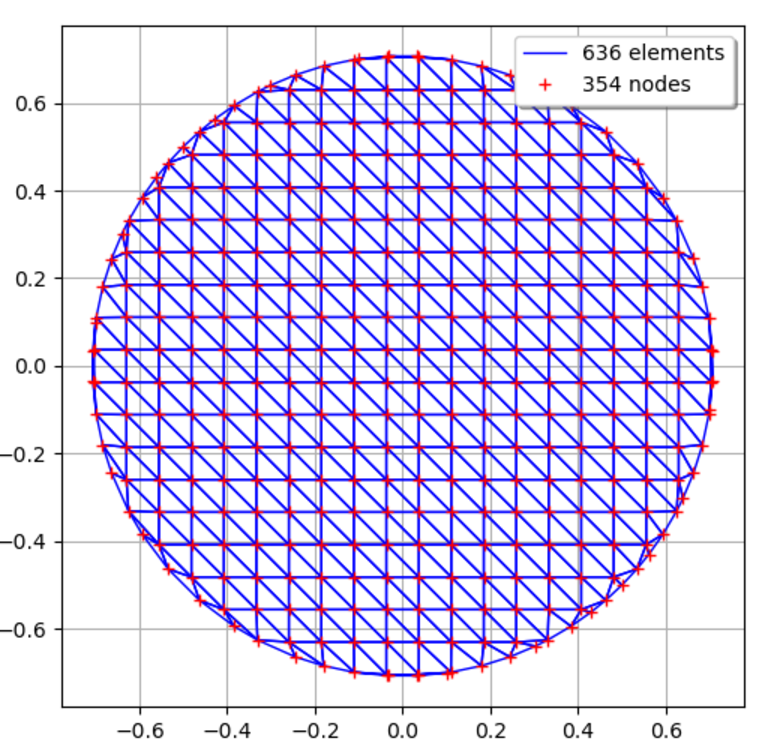
\includegraphics[scale=0.5]{images/meshP1Dim2-750.pdf}
\caption{Maillage d'intéret $M'$ en dimension 2}
\label{maillageInteretDim2}  
\end{center}
\end{figure}


\subsection{Dimension n=3}

On choisit $\bar{D}= [-1,1]^3$ et pour $m \in \mathbb{N}^{*}, \; m > 1$, le maillage $M$ sera caractérisé par des n\oe uds du type
\begin{equation*} \biggl (\biggl(-1 + \frac{2i}{m-1}, -1 + \frac{2j}{m-1}, -1 + \frac{2k}{m-1}\biggr)\biggr)_{(i,j,k) \in \llbracket 0;m-1 \rrbracket^3}  \end{equation*}
et leurs éléments tétraédriques sont décrits de la même façon qu'à la sous-section~\ref{choDim3} du chapitre~\ref{chapCholesky}.
Si on note $h_M$ le maximum des diamètres des éléments triangulaires qui composent le maillage $M$, $h_M = \sqrt{3} \cdot \frac{2}{m-1}$ .\\
Le nombre de n\oe uds $n_M = m^3$ variera entre $10$ et $10000$ et on ne considérera qu'une seule fonction de covariance $C$:
\begin{equation*} C(x,y) = \exp(-\|y-x\|_2^2)  \text{ pour } (x,y) \in (\bar{D})^2 \end{equation*}
~\\
Le maillage $M'$ est défini en deux temps. D'abord on discrétise le domaine $\bar{D}$ par un maillage $BE$ dont on
note $n_{BE}$ le nombre de n\oe uds. Pour \\$m_{BE} \in \mathbb{N}^{*}, \; m_{BE} > 1$, le maillage $BE$ sera caractérisé par des n\oe uds du type
\begin{equation*} \biggl (\biggl(-1 + \frac{2i}{m_{BE}-1}, -1 + \frac{2j}{m_{BE}-1}, -1 + \frac{2k}{m_{BE}-1}\biggr )\biggr)_{(i,j,k) \in \llbracket 0;m_{BE}-1 \rrbracket^3}  \end{equation*}
et leurs éléments tétraédriques sont décrits de la même façon qu'à la sous-section~\ref{choDim3} du chapitre~\ref{chapCholesky}.\\
Le nombre de n\oe uds $n_{BE} = m_{BE}^3$ est fixé à 1000.
On pose ensuite la fonction $f: (x,y,z)  \rightarrow 1 - \sqrt{x^2 + y^2 + z^3}$ et $v=1 - \frac{1}{\sqrt[3]{2}}$.
On obtient alors le maillage d'intérêt $M'$ en parcourant les éléments tétraédriques et en raisonnant de la façon suivante: si tous les sommets $s$
de l'élément vérifient $f(s)> v$ alors on enlève cet élément du maillage, sinon
si un sommet $s$ (mais pas tous) vérifie  $f(s)> v$ alors on modifie la position
du sommet $s$ de façon à ce qu'il vérifie $f(s) = v$.
Le maillage $M'$ ainsi obtenu est un maillage de la boule de centre $0$ et de rayon $v=\frac{1}{\sqrt[3]{2}}$.\\
\phantom{oyez}\\

\begin{figure}[h]
\begin{center}
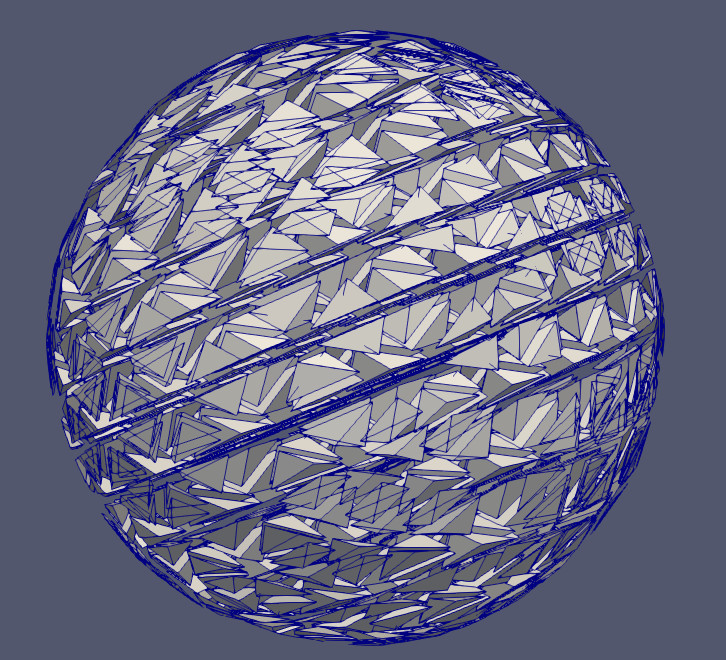
\includegraphics[scale=0.4]{images/meshP1Dim3-750.jpg}
\caption{Maillage d'intéret $M'$ en dimension 3}
\label{maillageInteretDim3}  
\end{center}
\end{figure}

\newpage

\subsection{Benchmarks}

\begin{table}[htbp]
\centering
\begin{tabular}{|>{\centering\arraybackslash}p{1.7cm} |>{\centering\arraybackslash}p{1.5cm} |>{\centering\arraybackslash}p{1.3cm} |>{\centering\arraybackslash}p{1.5cm} |}
\hline
Dimension & Nb de n\oe uds de $M'$ & Nb de n\oe uds de $M$ $n_{M}$ & Temps moyen d'une réalisation (en seconde)  \\
\hline
2 & 354 & 9 & 0.00457s  \\
\hline
2 & 354 & 100 & 0.00558s  \\
\hline
2 & 354 & 961 & 0.11667s  \\
\hline
2 & 354 & 10000 & 146.70s  \\
\hline
\hline
3 & 474 & 8 & 0.01782s  \\
\hline
3 & 474 & 64 & 0.02263s  \\
\hline
3 & 474 & 729 & 0.09118s  \\
\hline
3 & 474 & 9261 & 117.63s  \\
\hline
\end{tabular}
\end{table}

\begin{table}[htbp]
\centering
\begin{tabular}{|>{\centering\arraybackslash}p{1.7cm} |>{\centering\arraybackslash}p{1.5cm} |>{\centering\arraybackslash}p{1.3cm} |>{\centering\arraybackslash}p{1.5cm} |>{\centering\arraybackslash}p{1.5cm} |>{\centering\arraybackslash}p{1.2cm}|}
\hline
Dimension & Nb de n\oe uds de $M'$ & Nb de n\oe uds de $M$ $n_{M}$ & $h_M$ & Nb de réalisations & erreur $L^2$ \\
\hline
2 & 354 & 16 & 0.94280 & 250 & 0.09704   \\
\hline
2 & 354 & 16 & 0.94280 & 1000 & 0.13483   \\
\hline
2 & 354 & 16 & 0.94280 & 4000 & 0.11302   \\
\hline
2 & 354 & 16 & 0.94280 & 10000 & 0.11756   \\
\hline
\hline
2 & 354 & 121 & 0.28284 & 250 & 0.08694   \\
\hline
2 & 354 & 121 & 0.28284 & 1000 & 0.02646   \\
\hline
2 & 354 & 121 & 0.28284 & 4000 & 0.01703   \\
\hline
2 & 354 & 121 & 0.28284 & 10000 & 0.01040   \\
\hline
\hline
2 & 354 & 529 & 0.12856 & 250 & 0.16377   \\
\hline
2 & 354 & 529 & 0.12856 & 1000 & 0.01925   \\
\hline
2 & 354 & 529 & 0.12856 & 4000 & 0.01875   \\
\hline
2 & 354 & 529 & 0.12856 & 10000 & 0.00689   \\
\hline
\hline
2 & 354 & 1024 & 0.09123 & 250 & 0.04241   \\
\hline
2 & 354 & 1024 & 0.09123 & 1000 & 0.01526   \\
\hline
2 & 354 & 1024 & 0.09123 & 4000 & 0.04384   \\
\hline
2 & 354 & 1024 & 0.09123 & 10000 & 0.01988   \\
\hline
\hline
3 & 474 & 27 & 1.7320 & 250 & 0.43154 \\ 
\hline
3 & 474 & 27 & 1.7320 & 1000 & 0.43918 \\ 
\hline
3 & 474 & 27 & 1.7320 & 4000 & 0.45128 \\ 
\hline
3 & 474 & 27 & 1.7320 & 10000 & 0.45764 \\ 
\hline
\hline
3 & 474 & 125 & 0.86602 & 250 & 0.17489 \\ 
\hline
3 & 474 & 125 & 0.86602 & 1000 & 0.18455 \\ 
\hline
3 & 474 & 125 & 0.86602 & 4000 & 0.17802 \\ 
\hline
3 & 474 & 125 & 0.86602 & 10000 & 0.15349 \\
\hline
\hline
3 & 474 & 512 & 0.49487 & 250 & 0.14222 \\ 
\hline
3 & 474 & 512 & 0.49487 & 1000 & 0.07678 \\ 
\hline
3 & 474 & 512 & 0.49487 & 4000 & 0.07379 \\ 
\hline
3 & 474 & 512 & 0.49487 & 10000 & 0.06428 \\ 
\hline
\hline
3 & 474 & 1000 & 0.38490 & 250 & 0.11127 \\ 
\hline
3 & 474 & 1000 & 0.38490 & 1000 &  0.05500\\ 
\hline
3 & 474 & 1000 & 0.38490 & 4000 & 0.03705 \\ 
\hline
3 & 474 & 1000 & 0.38490 & 10000 & 0.02903 \\ 
\hline
\end{tabular}
\end{table}


\newpage

\begin{figure}[h]
\begin{center}
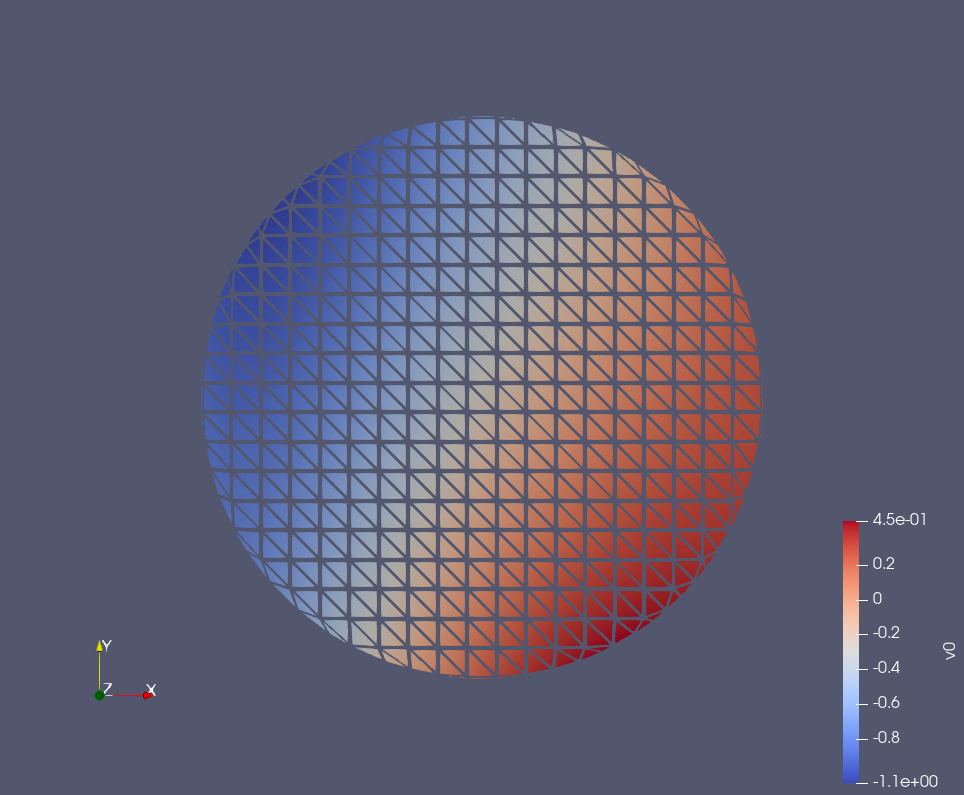
\includegraphics[scale=0.3]{images/meshP1Dim2-750-961.png}
\caption{Réalisation sur $M'$ en dimension 2 où $n_{M} = 961$ }
\label{ReaDim2-961}  
\end{center}
\end{figure}


\phantom{oyez}\\

\uppercase{à} des fins de comparaison, on rajoute ci-dessous un benchmark où on applique directement la méthode de Cholesky sur le maillage d'intérêt $M'$. On ne considère donc plus
le maillage $M$.\\
\phantom{oyez}

\begin{table}[htbp]
\centering
\begin{tabular}{|c |c |c |c |}
\hline
Dimension & Nb de n\oe uds de $M'$ & Nb de réalisations  & erreur $L^2$ \\
\hline
2 & 354 & 250 & 0.04956   \\
\hline
2 & 354 & 1000 & 0.01539   \\
\hline
2 & 354 & 4000 & 0.01319    \\
\hline
2 & 354 & 10000 & 0.01148   \\
\hline
\hline
3 & 474 & 250 & 0.17656 \\ 
\hline
3 & 474 & 1000 & 0.08154 \\ 
\hline
3 & 474 & 4000 & 0.03933 \\ 
\hline
3 & 474 & 10000 & 0.01620 \\ 
\hline
\end{tabular}
\end{table}



%\newpage

%\begin{figure}[h]
%\centering
%\begin{tikzpicture}
%\begin{axis} [ybar,
%height=3.2cm,
%width=10cm,
%axis x line=center,
%axis y line=center,
%xlabel style={below right},
%ylabel style={above left},
%xmin=5.0,
%xmax=9.5,
%xlabel = {$\ln(N_{rea})$},
%ylabel = {erreur $L^2$},
%ymin=0.0,
%ymax=0.25
%]
%\addplot coordinates {
%    (5.52146,0.17656) 
%    (6.90775,0.08154) 
%    (8.29404,0.03933) 
%    (9.21034,0.01620)
%};
%\end{axis}
%\end{tikzpicture}
%\caption{$n=2$, $n_M = 354$}
%\end{figure}











\small{
\bibliographystyle{plain-fr}
\bibliography{references}
}
\normalsize{}
%appendix
\appendix

\chapter{Base théorique pour la méthode spectrale}
\label{annexeA}
On introduit ici les outils théoriques permettant de comprendre la méthode
spectrale (voir chapitre~\ref{spectralMeth}). Pour la section~\ref{kloppi}, les terminologies de mesure complexe et de variation totale d'une mesure complexe ont
été puisées dans \cite{kloppCours}.



\section{Mesure matricielle}
\label{kloppi}
Soit $(\Lambda, \xi)$ un espace mesurable, $d \in \mathbb{N^*}$, $\mu = (\mu_{i,j})_{(i,j) \in \llbracket 1; d \rrbracket^2}$ une mesure vectorielle sur $(\Lambda, \xi)$ à valeurs dans $M_d(\mathbb{C})$ où les $\mu_{i,j}$ sont des mesures complexes dont on note leur variation totale $| \mu_{i,j} |$. \\

Pour $p \in [1, \infty[ $, on notera $L^{p}(\Lambda, \mu)$ l'ensemble des fonctions mesurables $f: \Lambda \rightarrow \mathbb{C}$ telles que $\forall (i,j) \in \llbracket 1; d \rrbracket^2, f \in L^{p}(\Lambda, |\mu_{i,j}|)$. 
L'une des conséquences immédiates est que pour $f \in L^{1}(\Lambda, \mu)$:\\

$\int_{\Lambda} f \mathrm{d}\mu = 
                                    \begin{pmatrix}
                                      \int_{\Lambda} f \mathrm{d}\mu_{1,1} & \cdots & \int_{\Lambda} f \mathrm{d}\mu_{1,d} \\
                                      \vdots &\ddots & \vdots \\
                                      \int_{\Lambda} f \mathrm{d}\mu_{d,1} & \cdots & \int_{\Lambda} f \mathrm{d}\mu_{d,d} \\
                                     \end{pmatrix}$  $\in M_d(\mathbb{C})$ est bien définie\\
         
         
~\\         
De plus on remarquera que comme la variation totale d'une mesure complexe est une mesure positive finie, pour $ (p,q) \in [1, \infty[^2 $ tel que $p \leq q, \;L^{q}(\Lambda, \mu) \subset L^{p}(\Lambda, \mu)$. D'où en particulier $L^{2}(\Lambda, \mu) \subset L^{1}(\Lambda, \mu)$.\\
~\\
Pour $p \in [1, \infty[ $, on peut noter aussi que $L^{p}(\Lambda, \mu) = L^{p}(\Lambda, \nu)$ où $\nu$ est une mesure positive sur $(\Lambda, \xi)$ telle que $\forall A \in \xi, \; \nu(A) = \displaystyle\sum_{(i,j) \in \llbracket 1;d \rrbracket^2} |\mu_{i,j}|(A) $. \\

\noindent D'où une structure d'espace de Banach de style $L^p$ telle que l'on connaît bien. Pour la suite, $\nu$ sera notée $\|\mu\|$. 

\section{Mesure stochastique orthogonale centrée et isométrie}

Soit $(\Omega, \mathcal{A}, \mathbb{P})$ un espace probabilisé, $\mu = (\mu_{i,j})_{(i,j) \in \llbracket 1;d \rrbracket^2}$ une mesure vectorielle sur $(\Lambda, \xi)$ à valeurs dans $M_d(\mathbb{C})$ où les $\mu_{i,j}$ sont des mesures complexes.\\

\noindent On note:
\begin{itemize}
\item $<.,.>$ l'application telle que $\forall (f,g) \in L^{2}(\Lambda, \mu)^2, \; <f,g> = \displaystyle\int_{\Lambda} f\bar{g} \mathrm{d}\mu$ \\

\item $L^{2}_{0}(\Omega, \mathcal{A}, \mathbb{P}; \mathbb{C}^{d})$, les vecteurs aléatoires centrés de $L^{2}(\Omega, \mathcal{A}, \mathbb{P}; \mathbb{C}^{d})$\\

\item $\|.\|_{L^{2}(\mathbb{P}; \mathbb{C}^d)}$ la norme hilbertienne de $L^{2}(\Omega, \mathcal{A}, \mathbb{P}; \mathbb{C}^{d}) \;$ telle que $\|X\|_{L^{2}(\mathbb{P}, \mathbb{C}^d)}^2$ vaut $ \mathbb{E}(\|X\|^{2}_{2})$, où $\|.\|_{2}$ est la norme hermitienne naturelle dans $\mathbb{C}^{d}$\\
\end{itemize}

\begin{remark}$L^{2}_{0}(\Omega, \mathcal{A}, \mathbb{P};\mathbb{C}^{d})$ est un sous-espace vectoriel fermé de \\$L^{2}(\Omega, \mathcal{A}, \mathbb{P}; \mathbb{C}^{d})$.\end{remark}

\begin{definition}
Soit $I: L^{2}(\Lambda, \mu)  \rightarrow L^{2}_{0}(\Omega, \mathcal{A}, \mathbb{P}; \mathbb{C}^{d})$ une application. On dit que $I$ est une mesure stochastique orthogonale centrée (m.s.o.c) de mesure structurelle (ou de base) $\mu$ si $\forall f \in L^{2}(\Lambda, \mu)$:
\begin{equation}
<f,f>\;=\;\mathbb{E}(I(f)I(f)^{*})
\end{equation}

\noindent Et si tel est le cas, on définit la mesure stochastique associée à $I$ comme l'application $\phi: \xi \rightarrow L^{2}_{0}(\Omega, \mathcal{A}, \mathbb{P}; \mathbb{C}^{d})$ telle que $\forall B \in \xi, \; \phi(B)= I(\mathds{1}_{B})$.
\end{definition}

\begin{remark}
\begin{equation*}
 \forall f \in L^{2}(\Lambda, \mu), \; <f,f>\;=\;\mathbb{E}(I(f)I(f)^{*}) \end{equation*}
\begin{equation} \iff \end{equation}
\begin{equation*}
\forall (f,g) \in L^{2}(\Lambda, \mu)^2,  <f,g>\;=\;\mathbb{E}(I(f)I(g)^{*})
\end{equation*}
\end{remark}
~\\
Supposons maintenant que $I$ est une m.s.o.c. D'où les propriétés suivantes:
\begin{itemize}
\item  $tr(\mu) = \displaystyle\sum_{i=1}^{d} \mu_{i,i}$ est une mesure positive sur $(\Lambda,\xi)$ (mesure-trace de $\mu$) \\ 


\item  $\forall (i,j) \in \llbracket 1;d\rrbracket^2, \;\forall (f,g) \in L^{2}(\Lambda, \mu)^2$:\\$\; |\int_{\Lambda} f\bar{g} d\mu_{i,j} | \leq (\int_{\Lambda} |f|^2 dtr(\mu))^{\frac{1}{2}}(\int_{\Lambda} |g|^2 dtr(\mu))^{\frac{1}{2}}$\\


\item $\forall A \in \xi,\; |\mu_{i,j}(A)| \leq |\mu_{i,j}|(A) \leq tr(\mu)(A)$ (la mesure-trace contrôle tous les coefficients de la mesure vectorielle $\mu$)\\

\item $L^{2}(\Lambda, \mu) = L^{2}(\Lambda, tr(\mu))$ et $I$ est une isométrie de $L^{2}(\Lambda, tr(\mu))$ dans $L^{2}_{0}(\Omega, \mathcal{A}, \mathbb{P}, \mathbb{C}^{d})$\\



\item $\phi$ la mesure stochastique associée à $I$ est bien une mesure stochastique sur $(\Lambda, \xi)$ à valeurs dans $L^{2}_{0}(\Omega, \mathcal{A}, \mathbb{P}, \mathbb{C}^{d})$ i.e que pour toute famille dénombrable de parties mesurables 2 à 2 disjointes $(A_j)_{j \in \mathbb{N}}, \;$\\$\phi(\displaystyle\cup_{j \in \mathbb{N}} A_j) =  \displaystyle\sum_{j \in \mathbb{N}} \phi(A_j) $ (somme au sens de la norme $\|.\|_{L^{2}(\mathbb{P}, \mathbb{C}^d)}$)\\

\end{itemize}

\begin{definition}
\label{A22}
Soit $I: L^{2}(\Lambda, \mu)  \rightarrow L^{2}_{0}(\Omega, \mathcal{A}, \mathbb{P}; \mathbb{C}^{d})$ une m.s.o.c de mesure de base $\mu$ dont on note $\phi$ la mesure stochastique associée. On définit pour $f \in L^{2}(\Lambda, \mu)$, l'intégrale de Wiener de $f$ associée à la mesure stochastique $\phi$ ainsi: 

\begin{equation} \int_{\Lambda} f(\lambda) \phi(d\lambda) = I(f) \end{equation}

\noindent Et pour toute partie mesurable $\Gamma \subset \Lambda$, pour tout $f \in L^{2}(\Lambda, \mu)$, on définit:
$\int_{\Gamma} f(\lambda) \phi(d\lambda) = \int_{\Lambda} \mathds{1}_{\Gamma}(\lambda)f(\lambda) \phi(d\lambda) = I(\mathds{1}_{\Gamma}f)$\\
\end{definition}

\begin{remark} Si on a une mesure stochastique $\phi_2$ issue d'une autre m.s.o.c $I_2$ de mesure de base aussi $\mu$, alors pour démontrer que $\phi_2 = \phi$, il suffit juste de démontrer que l'on dispose de $A$ une partie dense de $L^{2}(\Lambda, tr(\mu))$ telle que l'intégrale de Wiener associée à $\phi$ et celle associée à $\phi_2$ sont égales pour tout élément de $A$ (ce qui revient à dire $I_{|A} = (I_{2})_{|A} $) \end{remark}



\section{Sur l'existence d'une m.s.o.c associée à un champ aléatoire}

\noindent Pour plus de détails sur les résultats généraux de cette section, voir \cite{alma991000210539806616}.\\
~\\Considérons $(\Omega, F, \mathbb{P})$ un espace probabilisé, $n$ et $d$ deux entiers naturels non nuls et $X: \mathbb{R}^n \times \Omega \rightarrow \mathbb{R}^d$ un champ aléatoire. On émet l'hypothèse suivante:
\begin{hypothesis}
$X$ est d'ordre 2, centré, continue en moyenne quadratique, faiblement stationnaire d'ordre 2. \label{hypFond}
\end{hypothesis}

\noindent On note $R: \mathbb{R}^n \rightarrow M_d(\mathbb{C})$ la fonction d'autocovariance de $X$.

\subsection{Mesure spectrale}

\begin{theorem}
Sous l'hypothèse~\ref{hypFond}, on dispose d'une unique mesure vectorielle $\mu = (\mu_{i,j})_{(i,j) \in \llbracket 1;d \rrbracket^2} $ sur $(\mathbb{R}^n, \mathcal{B}(\mathbb{R}^n))$ à valeurs dans l'ensemble des matrices hermitiennes semi-définies positives de $M_d(\mathbb{C})$, dont les $\mu_{i,j}$ sont des mesures complexes et telle que: \begin{equation} \forall t \in \mathbb{R}^n, R(t) = \displaystyle\int_{\mathbb{R}^n} \exp(i<t,\omega>_{n}) d\mu(\omega) \end{equation}
\end{theorem}

\noindent ($<.,.>_{n}$ est le produit scalaire usuel dans $\mathbb{R}^n$)

\begin{definition}
Avec les notations du précédent théorème, on appelle $\mu$ la mesure spectrale matricielle ou juste mesure spectrale de $X$ et on la note $M_X$.
\end{definition}

\begin{property}
$tr(M_X)$ est une mesure positive sur $(\mathbb{R}^n, \mathcal{B}(\mathbb{R}^n))$. 
\end{property}

\begin{property}
$\forall A \in \mathcal{B}(\mathbb{R}^n), \; M_X(A) = \overline{M_X(-A)}$ donc
en particulier $tr(M_X)(A) = tr(M_X)(-A)$.
\end{property}

\subsection{Densité spectrale}

\begin{definition}
Si les mesures $(M_{X})_{i,j}$ sont à densité par rapport à la mesure de Lebesgue $d\omega$ de $\mathbb{R}^n$ alors on dispose de $S = (S_{i,j})_{(i,j) \in \llbracket 1; d \rrbracket^2}  $ une application mesurable allant de $\mathbb{R}^n$ dans $M_d(\mathbb{C})$, $d\omega$-intégrable et unique à un ensemble de mesure nulle près par rapport à la mesure $d\omega$, telle que:

\begin{equation} \forall A \in \mathcal{B}(\mathbb{R}^n),  M_X(A) = \displaystyle\int_{A} S(\omega)d\omega \end{equation}
\\ Donc $\forall (i,j) \in \llbracket 1; d \rrbracket^2, \; \forall A \in \mathcal{B}(\mathbb{R}^n), (M_{X})_{i,j}(A) = \displaystyle\int_{A} S_{i,j}(\omega)d\omega$\\
~\\On appelle $S$ la densité spectrale de $X$ et on la note $S_X$.

\end{definition}
~\\
Supposons jusqu'à la fin de cette sous-section que le champ $X$ admet une
densité spectrale $S_X$. On observe alors ces propriétés:\\
\begin{itemize}
\item $\forall t \in \mathbb{R}^n, R(t) = \displaystyle\int_{\mathbb{R}^n} \exp(i<t,\omega>_{n})S_X(\omega) d\omega$

\item  $S_X$ est $d\omega$-presque partout hermitienne semi-définie positive

\item Pour presque tout $\omega \in \mathbb{R}^n$ , $S_X(-\omega) = \overline{S_X(\omega)}$

\item Si  $\|R\|_F$ est dans $L^1(\mathbb{R}^n,dt)$ (où $dt = d\omega$)  alors $S_X$ peut être décrite explicitement via une transformée de Fourier: \\$\forall \omega \in \mathbb{R}^n, S_X(\omega) = (2\pi)^{-n}\displaystyle\int_{\mathbb{R}^n} \exp(-i<\omega,t>_n)R(t) dt $. \\
\end{itemize}

\begin{remark}
Tous les coefficients de $R$ sont dans $L^1(\mathbb{R}^n,dt)$ si et seulement si
$\|R\|_F$ est dans $L^1(\mathbb{R}^n,dt)$ ($\;\|.\|_F$ désigne la norme de Frobenius).
\end{remark}


\subsection{Densité spectrale fréquentielle}
\label{DSFr}
Mettons en avant maintenant le fait que la notation $\omega$ souligne la notion de pulsation rencontrée en physique mais il est possible que l'on souhaite parler non pas de pulsation mais de fréquence $f = \frac{\omega}{2\pi}$. C'est pourquoi l'on définit une autre densité spectrale que l'on appelle densité spectrale fréquentielle. On suppose de nouveau que le champ aléatoire $X$ admet une densité spectrale $S_X$.

\begin{definition}
On définit alors la densité spectrale fréquentielle de $X$ comme l'application $S^{fr}_X : \mathbb{R}^n \rightarrow M_d(\mathbb{R})$ telle que:
\begin{equation*}
\forall f \in \mathbb{R}^n, S^{fr}_X(f) = (2\pi)^{n}S_X(2\pi f)
\end{equation*}
\end{definition}

\begin{property}
Si $\|R\|_F$ est dans $L^1(\mathbb{R}^n,dt)$ alors $S^{fr}_X$ peut être totalement
décrite par une transformée de Fourier de la fonction d'autocovariance $R$: \begin{equation*} \forall f \in \mathbb{R}^n,\;  S^{fr}_X(f) = \displaystyle\int_{\mathbb{R}^n} \exp(-2\pi i<f,t>_n)R(t) dt \end{equation*}
\end{property}


\section{Représentation spectrale de X}
\label{repSpecSect}
Sous l'hypothèse \ref{hypFond}, on a pu exhiber dans la section précédente la notion de mesure spectrale matricielle mais on peut aller plus loin et démontrer l'existence d'une unique mesure stochastique associée à $X$, $\phi_X$, issue d'une unique m.s.o.c. $I_X$ décrivant totalement $X$. Précisément sous l'hypothèse \ref{hypFond}:

\begin{theorem}
\label{repSpec} Il existe une unique mesure stochastique $\phi_X : \mathcal{B}(\mathbb{R}^n) \rightarrow L^{2}_{0}(\Omega, \mathcal{A}, \mathbb{P}, \mathbb{C}^{d})$ associée à une unique m.s.o.c $I_X$ de mesure de base la mesure spectrale $M_X$, telle que:
\begin{equation*}
\forall t \in \mathbb{R}^n, X(t,.) = \displaystyle\int_{\mathbb{R}^n} \exp(i<t,\omega>_{n}) \phi_X(d\omega)
\end{equation*}

\noindent Si de plus $X$ est un champ gaussien, $\phi_X$ est une mesure stochastique gaussienne centrée i.e $\forall A \in \mathcal{B}(\mathbb{R}^n), \phi_X(A)$ est un vecteur gaussien à valeurs dans $\mathbb{C}^d$, centré, dont la matrice de covariance complexe vaut $\mathbb{E}(\phi_X(A)\phi_X(A)^{*}) \; ( = M_X(A))$
\end{theorem}

\begin{property}
$\forall f \in L^2(\mathbb{R}^n, M_X),\; \overline{I_X(f)} = I_X(\bar{f}(-\cdot))$
\end{property}

\begin{remark} \noindent Cette première propriété est inspirée de la page 52 du livre de Prigarin \cite{bookPS}. \end{remark}

\begin{property}
$\forall A \in \mathcal{B}(\mathbb{R}^n),\; \phi_X(A) = \overline{\phi_X(-A)}$
\end{property}

\begin{property}$\forall (A,B) \in \mathcal{B}(\mathbb{R}^n)^2, \; \mathbb{E}(\phi_X(A)\phi(B)_{X}^{\top}) = M_X(A \cap (-B))$ 
\end{property}

\begin{property}
Si $X$ est un champ gaussien alors toute famille d'éléments de $I_X(L^{2}(\mathbb{R}^n, M_X))$ indexée par un ensemble $D$ quelconque est un processus gaussien centré. 
\end{property}


\chapter{Code pour les tests numériques}
\label{codeNumAnnexe}
Du code utilisant la librairie OpenTURNS a été créé pour les tests numériques.
Ce code est disponible sous demande sur un dépôt git (Github). On se propose donc ici de décrire la structure des dossiers/fichiers de ce dépôt.
Tout est rassemblé dans un même dossier de nom Benchmarks.

\section{Dossier CholeskyMethod}
\label{dossCholeskyM}
Le dossier est composé de deux fichiers. Le fichier testTool.py contient une unique fonction
du nom checkCovariance() qui consiste à partir un échantillon de réalisations de déterminer l'erreur
$L^2$ (voir la sous-section~\ref{quantifErreur} du chapitre~\ref{chapCholesky}) par rapport à une matrice $\Sigma$ construite de la même façon qu'au chapitre~\ref{introProb} à l'aide
du maillage où on effectue les réalisations et d'une fonction de covariance $C$. Ce fichier existe dans tous les dossiers qui seront décrits dans les sections suivantes
mais pour le dossier SpectralMethod, le fichier testTool.py sera agrémenté d'autres fonctions.
Le second fichier se nomme cholesky.py et il contient des tests numériques qui sont détaillés
au chapitre~\ref{chapCholesky} à la section~\ref{errConvCholesky}.
\section{Dossier HmatrixMethod}
Le dossier est composé de deux fichiers. Le fichier testTool.py et
le fichier Hmatrix.py qui contient des tests numériques qui sont détaillés
au chapitre~\ref{hmatrixchapter} à la section~\ref{hmatrixerrconv}.

\section{Dossier GalliGaoGibbsMethod}
Le dossier est composé de deux fichiers. Le fichier testTool.py et
le fichier GGG.py qui contient des tests numériques qui sont détaillés
au chapitre~\ref{GGGMethod} à la section~\ref{gggErrConv}.

\section{Dossier SpectralMethod}
\label{dossSpec}
Le dossier est composé de 11 fichiers et par la suite, quand on parlera de densité spectrale, on
sous-entendra densité spectrale fréquentielle (voir la sous-section~\ref{DSFr} de l'annexe~\ref{annexeA}). Les fichiers
mySpectralGaussianProcess1D.py, mySpectralGaussianProcess2D.py et mySpectralGaussianProcess3D.py\\
contiennent l'implémentation de la méthode spectrale en fonction de la dimension d'entrée
du processus $X: \mathbb{R}^n \times \Omega \rightarrow \mathbb{R}^d$ (n=1, 2 ou 3). Ces
fichiers ne contiennent qu'une classe, celle qui implémente la méthode spectrale et
qui porte le même nom que le fichier sauf que ça commence par une majuscule. La classe, en plus
du constructeur, contient systématiquement les méthodes utilisables suivantes: getRealization(),
getSample(), getOutputDimension() et getMesh().\\

Les fichiers estimationSpectraleDim1.py, estimationSpectraleDim2.py, estimationSpectraleDim3.py contiennent
l'implémentation de l'estimateur de la densité spectrale évoquée à la section~\ref{erreurConvSpectral}
du chapitre~\ref{spectralMeth}. Ces fichiers ne contiennent qu'une classe, celle qui implémente l'estimateur
de la densité spectrale. La classe, en plus du constructeur, contient systématiquement la méthode utilisable
buildFromSample() qui évalue l'estimateur en fonction des réalisations sur le maillage formé par les points de simulation
et (en utilisant les notations des sections~\ref{subdivdomspec} et~\ref{subdiv} du chapitre~\ref{spectralMeth}) en
fonction de $N_1, \dots, N_n$ et de $T_1 - \Delta t_1 , \cdots, T_n - \Delta t_n  = (N_n- 1)\Delta t_n$. Plus explicitement,
la syntaxe se présente ainsi:
\begin{equation*} buildFromSample(sample, [N_1, \cdots, N_n], [T_1 - \Delta t_1 , \cdots, T_n - \Delta t_n]) \end{equation*}
~\\
Le fichier spectralModels.py contient l'implémentation de plusieurs densités spectrales:

\begin{equation} S(f) = \frac{1}{2A} \mathds{1}_{[-A,A]}(f) \tag{S1} \label{S1}\end{equation}
\begin{equation} S(f) = S(f_1,\cdots,f_n) = \sigma^{2} (\pi \theta)^{\frac{n}{2}} exp(-\pi^{2} \theta \|f\|_{2}^{2}) . I_{d} \tag{S2}\label{S2}\end{equation}
\begin{equation} S(f) = S(f_1,f_2,f_3) = \frac{8\pi a}{(a^2 +(2\pi)^{2} \|f\|_{2}^{2})^{2}} \tag{S3}\label{S3}\end{equation}
\begin{equation} S(f) = S(f_1,f_2) = \sigma^2 b_1.b_2.\pi.exp(-\pi^2 (b_1^2 f_1^2 + b_2^2 f_2^2) ) \tag{S4}\label{S4}\end{equation}

\noindent Les fonctions d'autocovariance associées à ces densités sont respectivement:

\begin{equation} R(t) = \frac{sin(2\pi A t)}{2\pi A t}  \tag{R1}\label{R1} \end{equation}
\begin{equation} R(t) = R(t_1,\cdots,t_n) = \sigma^{2} exp(- \frac{\|t\|_{2}^{2}}{\theta}) . I_{d} \tag{R2}\label{R2}\end{equation}
\begin{equation} R(t) = R(t_1,t_2,t_3) = exp(-a \|t\|_{2})  \tag{R3}\label{R3}\end{equation}
\begin{equation} R(t) = R(t_1,t_2) = \sigma^2 exp(-(t_1/b_1)^{2} - (t_2/b_2)^{2}) \tag{R4}\label{R4}\end{equation}


\noindent Les densités \eqref{S1}, \eqref{S3}, et \eqref{S4} sont implémentées par les classes respectives
UniformSpectralModel, SpectralModelofExponential3D1D et SpectralModelofAnExponential2D1D. La densité
\eqref{S2} est implémentée de façon générale par la classe GaussianSpectralModel mais dans
le cas où $n=1$, on utilise la classe GaussianSpectralModelDim1 afin d'éviter des problèmes
de compatibilité avec la librairie OpenTURNS.\\

Le fichier tool.py contient deux méthodes. Toujours en utilisant
les notations des sections~\ref{subdivdomspec} et~\ref{subdiv} du chapitre~\ref{spectralMeth},
la méthode createSpatialSteps()
permet de déduire la liste $[\Delta t_1, \cdots, \Delta t_n]$ à partir
de la liste $[N_1 - 1, \cdots, N_n -1]$ et la liste $[T_1 - \Delta t_1 , \cdots, T_n - \Delta t_n]$.
En effet pour $i \in \llbracket 1;n \rrbracket, \; \Delta t_i = \frac{T_i - \Delta t_i}{N_i - 1}$.
Plus explicitement, la syntaxe se présente ainsi:
\begin{equation*} [\Delta t_1, \cdots, \Delta t_n] = createSpatialSteps([N_1 - 1, \cdots, N_n -1], [T_1 - \Delta t_1 , \cdots, T_n - \Delta t_n]) \end{equation*}
\noindent La méthode createSpectralSteps() permet de déduire la liste $[\Delta f_1, \cdots, \Delta f_n]$ à
partir de  la liste $[T_1, \cdots, T_n]$. En effet pour $i \in \llbracket 1;n \rrbracket, \; \Delta f_i = \frac{1}{T_i}$.
La syntaxe se présente ainsi:
\begin{equation*} [\Delta f_1, \cdots, \Delta f_n] = createSpatialSteps([T_1, \cdots, T_n]) \end{equation*}


Le fichier userDefinedSpectralModel.py contient une classe de même nom (à une majuscule près) ainsi qu'une fonction utile à la classe.
Cette classe permet de définir une densité spectrale $S$ sur un pavé $D_f = [-f_{max,1}, f_{max,1}] \times \cdots \times [-f_{max,n}, f_{max,n}]$.
Chaque arête $[-f_{max,j}, f_{max,j}]$ a été subdivisée en $N_j$ intervalles de longueur $\Delta f_j$
de centres respectifs $f_{j,1}, \cdots, f_{j,N_j}$. La densité spectrale $S$ est définie
sur $D_f$ par morceaux et est constante sur les pavés
\begin{equation*}
\tilde{M}_{(k_1,\cdots,k_n)} = [f_{1,k_1} -\frac{\Delta f_1}{2}, f_{1,k_1} + \frac{\Delta f_1}{2} [ \times \cdots \times [f_{n,k_n} -\frac{\Delta f_n}{2}, f_{n,k_n} + \frac{\Delta f_n}{2}[
\end{equation*}
où $(k_1,\cdots,k_n) \in \llbracket 1;N_1 \rrbracket \times \cdots \times \llbracket 1;N_n \rrbracket $.\\

Le fichier testTool.py contient de multiples fonctions. On a la fonction checkCovariance() évoquée à la section~\ref{dossCholeskyM}.
On rajoute ensuite la fonction createStationaryCovarianceModel() qui à partir d'un maillage $M$ donné et d'une
fonction d'autocovariance $R$ allant de $\mathbb{R}^{n}$ dans $\mathbb{R}$ ($d$, la dimension de sortie vaut ici $1$)
crée un modèle gaussien de covariance sur le maillage $M$, c'est-à-dire en utilisant les notations du
chapitre~\ref{introProb} (où $m$ désigne le nombre de n\oe uds du maillage) que l'on simule
le vecteur gaussien $\mathcal{N}(0_{\mathbb{R}^{dm}},\Sigma)$ où pour $n_i$ et $n_j$ deux n\oe uds du maillage
, on a $\Sigma_{i,j} = C(n_i,n_j) = R(n_j - n_i)$.\\
Ensuite pour $K \in \llbracket 1;3 \rrbracket$,
on dispose des fonctions suivantes:  getNormInfDim$K$() et compareSpectralModelsNormInfDim$K$().
Les deux fonctions nécessitent une famille $F$ de points de l'espace descriptibles de la
même façon que les points \begin{equation*} ((f_{1,k_1}, \cdots, f_{n,k_n}))_{ k \in \llbracket 1;N_1 \rrbracket \times \cdots \times \llbracket 1;N_n \rrbracket} \end{equation*}
évoqués plus tôt pour le fichier userDefinedSpectralModel.py. Pour getNormInf-
Dim$K$(),
avec l'information d'une densité spectrale $S$, la fonction va chercher le point dont la norme de Frobenius de
son image par $S$ est la plus élevée et retournera cette valeur. Pour la fonction compareSpectralModelsNormInfDim$K$() avec l'information de deux densités
spectrales $S_1$ et $S_2$, la fonction va chercher le point dont la norme de Frobenius de
son image par $S_2 - S_1$ est la plus élevée et retournera cette valeur. C'est donc cette
fonction que l'on utilisera pour évaluer l'erreur entre deux densités spectrales en les points de la famille $F$.\\
La dernière fonction s'y trouvant est la fonction graphOfTwoModelsInputDim1OutputDim1() qui va dessiner
le graphe de deux densités spectrales \\allant de $\mathbb{R}$ dans $\mathbb{R}$ dont on considère
les valeurs pour les points de $F$.\\

Le dernier fichier à évoquer est le fichier qui décrit des tests numériques:
spectral.py. Le détail des tests effectués se trouvent dans la section~\ref{erreurConvSpectral}
du chapitre~\ref{spectralMeth}.


\section{Dossier P1InterpolationMethod}

Le dossier est composé de trois fichiers. Le fichier testTool.py,
le fichier P1Interpolation.py qui contient des tests numériques qui sont détaillés
au chapitre~\ref{P1Interpol} à la section~\ref{P1interpolConvErr} et le fichier P1InterpolationGaussianProcess.py.
Ce dernier fichier contient la classe qui implémente la méthode par $\mathbb{P}_{1}$-interpolation.
Cette classe de nom P1InterpolationGaussianProcess contient, en plus du \\constructeur, la méthode
getRealization(), getSample(), getMesh(), getOutputDimension(), changeEnvelopingProcess()
et getEnvelopingMesh(). Ici ce que l'on désigne comme EnvelopingProcess désigne le champ gaussien simulé au niveau des n\oe uds du maillage EnvelopingMesh
qui n'est rien d'autre que le maillage $M$ évoqué au début de la section~\ref{P1interpolConvErr} du chapitre~\ref{P1Interpol}.


\end{document}
